% Document type, global settings, and packages

\documentclass[12pt]{report}   %12 point font for Times New Roman
\usepackage{graphicx}  %for images and plots
\usepackage{subcaption}
\usepackage[letterpaper, left=1in, right=1in, top=1in, bottom=1in]{geometry}
\usepackage{setspace}  %use this package to set linespacing as desired
\usepackage{times}  %set Times New Roman as the font
\usepackage[explicit]{titlesec}  %title control and formatting
\usepackage[titles]{tocloft}  %table of contents control and formatting
\usepackage[backend=bibtex, sorting=none, bibstyle=ieee, style=numeric]{biblatex}  %reference manager
\usepackage{appendix}  %for appendices
\usepackage{rotating}  %for rotated, landscape images
\usepackage[normalem]{ulem}  %for underlined section titles
\usepackage{textcomp} % for text symbols such as copyright etc. 
\usepackage{indentfirst} % To indent the first line of every paragraph
\usepackage{booktabs,array,arydshln} %for better table formatting. 
\usepackage{amsmath} %for formula formatting
\usepackage{ amssymb }
\usepackage{gensymb}
\usepackage[T1]{fontenc} % improved font encoding
\usepackage[utf8]{inputenc} % for better handling of non-ASCII characters
%\usepackage{newtxtext} % font choice
\usepackage{newtxmath} 
%\usepackage{lmodern} % font choice 
%\usepackage[bookmarks=true, hidelinks]{hyperref}
\usepackage[hidelinks]{hyperref}
\usepackage{physics}
\usepackage{lineno}
\usepackage{cancel}

\linenumbers

% My Definitions
\def\invfb{fb\textsuperscript{-1}}

% Bibliography
%Add your bibliography file here
\bibliography{references}

% prevent certain fields in references from printing in bibliography
\AtEveryBibitem{\clearfield{issn}}
\AtEveryBibitem{\clearlist{issn}}

\AtEveryBibitem{\clearfield{language}}
\AtEveryBibitem{\clearlist{language}}

\AtEveryBibitem{\clearfield{doi}}
\AtEveryBibitem{\clearlist{doi}}

\AtEveryBibitem{\clearfield{url}}
\AtEveryBibitem{\clearlist{url}}

\AtEveryBibitem{%
  \ifentrytype{online}
    {}
    {\clearfield{urlyear}\clearfield{urlmonth}\clearfield{urlday}}}


% Start of Dissertation Document

\begin{document}
\doublespacing  %set line spacing to double by default through out the document. This can be overwritten when necessary

% Title Page (No page number)
%This is the tile page of your dissertation
%Please type below title of your dissertation and your name
%change the year if neccessary

\begin{titlepage}
\begin{center}

\begin{singlespacing}
\vspace*{6\baselineskip}
[ATLAS Semivisible Jets]\\
\vspace{3\baselineskip}
[Elena Laura Busch]\\
\vspace{18\baselineskip}
Submitted in partial fulfillment of the\\
requirements for the degree of\\
Doctor of Philosophy\\
under the Executive Committee\\
of the Graduate School of Arts and Sciences\\
\vspace{3\baselineskip}
COLUMBIA UNIVERSITY\\
\vspace{3\baselineskip}
\the\year
\vfill


\end{singlespacing}

\end{center}
\end{titlepage}





% Copyright  Page (No page number)


\begin{titlepage}
\begin{singlespacing}
\begin{center}

\vspace*{35\baselineskip}

\textcopyright  \,  \the\year\\
\vspace{\baselineskip}	
Elena Laura Busch\\
\vspace{\baselineskip}	
All Rights Reserved
\end{center}
\vfill

\end{singlespacing}
\end{titlepage}


% Abstract (No page number)
\pagenumbering{gobble}
%Abstract Page

\begin{titlepage}
\begin{center}

\vspace*{5\baselineskip}
\textbf{\large Abstract}

[ATLAS Semivisible Jets]

[Elena Laura Busch]
\end{center}
\begin{flushleft}
\hspace{10mm}Abstract of dissertation. In the abstract, you must (1) present the problem of the thesis/dissertation, (2) discuss the materials and methods used, and (3) state the conclusions reached. Individual chapters should not have abstracts.Abstract of dissertation. In the abstract, you must (1) present the problem of the thesis/dissertation, (2) discuss the materials and methods used, and (3) state the conclusions reached. Individual chapters should not have abstracts.Abstract of dissertation. In the abstract, you must (1) present the problem of the thesis/dissertation, (2) discuss the materials and methods used, and (3) state the conclusions reached. Individual chapters should not have abstracts.Abstract of dissertation. In the abstract, you must (1) present the problem of the thesis/dissertation, (2) discuss the materials and methods used, and (3) state the conclusions reached. Individual chapters should not have abstracts.Abstract of dissertation. In the abstract, you must (1) present the problem of the thesis/dissertation, (2) discuss the materials and methods used, and (3) state the conclusions reached. Individual chapters should not have abstracts.Abstract of dissertation. In the abstract, you must (1) present the problem of the thesis/dissertation, (2) discuss the materials and methods used, and (3) state the conclusions reached. Individual chapters should not have abstracts.Abstract of dissertation. In the abstract, you must (1) present the problem of the thesis/dissertation, (2) discuss the materials and methods used, and (3) state the conclusions reached. Individual chapters should not have abstracts.Abstract of dissertation. In the abstract, you must (1) present the problem of the thesis/dissertation, (2) discuss the materials and methods used, and (3) state the conclusions reached. Individual chapters should not have abstracts.Abstract of dissertation. In the abstract, you must (1) present the problem of the thesis/dissertation, (2) discuss the materials and methods used, and (3) state the conclusions reached. Individual chapters should not have abstracts.Abstract of dissertation. In the abstract, you must (1) present the problem of the thesis/dissertation, (2) discuss the materials and methods used, and (3) state the conclusions reached. Individual chapters should not have abstracts.Abstract of dissertation. In the abstract, you must (1) present the problem of the thesis/dissertation, (2) discuss the materials and methods used, and (3) state the conclusions reached. Individual chapters should not have abstracts.Abstract of dissertation. In the abstract, you must (1) present the problem of the thesis/dissertation, (2) discuss the materials and methods used, and (3) state the conclusions reached. Individual chapters should not have abstracts.Abstract of dissertation. In the abstract, you must (1) present the problem of the thesis/dissertation, (2) discuss the materials and methods used, and (3) state the conclusions reached. Individual chapters should not have abstracts.Abstract of dissertation. In the abstract, you must (1) present the problem of the thesis/dissertation, (2) discuss the materials and methods used, and (3) state the conclusions reached. Individual chapters should not have abstracts.Abstract of dissertation. In the abstract, you must (1) present the problem of the thesis/dissertation, (2) discuss the materials and methods used, and (3) state the conclusions reached. Individual chapters should not have abstracts.Abstract of dissertation. In the abstract, you must (1) present the problem of the thesis/dissertation, (2) discuss the materials and methods used, and (3) state the conclusions reached. Individual chapters should not have abstracts.Abstract of dissertation. In the abstract, you must (1) present the problem of the thesis/dissertation, (2) discuss the materials and methods used, and (3) state the conclusions reached. Individual chapters should not have abstracts.Abstract of dissertation. In the abstract, you must (1) present the problem of the thesis/dissertation, (2) discuss the materials and methods used, and (3) state the conclusions reached. Individual chapters should not have abstracts.Abstract of dissertation. In the abstract, you must (1) present the problem of the thesis/dissertation, (2) discuss the materials and methods used, and (3) state the conclusions reached. Individual chapters should not have abstracts.

\end{flushleft}
\vspace*{\fill}
\end{titlepage}



% Table of Contents
%\currentpdfbookmark{Table of Contents}{TOC}
% Format for Table of Contents
\pagenumbering{roman}
\setcounter{page}{1} 
\renewcommand{\cftchapdotsep}{\cftdotsep}  %add dot separators
\renewcommand{\cftchapfont}{\normalfont}  %set title font weight that shows up on TOC
\renewcommand{\cftchappagefont}{}  %set page number font weight
\renewcommand{\cftchappresnum}{Chapter }
\renewcommand{\cftchapaftersnum}{:}
\renewcommand{\cftchapnumwidth}{5em}
\renewcommand{\cftchapafterpnum}{\vskip\baselineskip} %set correct spacing for entries in single space environment
\renewcommand{\cftsecafterpnum}{\vskip\baselineskip}  %set correct spacing for entries in single space environment
\renewcommand{\cftsubsecafterpnum}{\vskip\baselineskip} %set correct spacing for entries in single space environment
\renewcommand{\cftsubsubsecafterpnum}{\vskip\baselineskip} %set correct spacing for entries in single space environment

% My commands
\newcommand{\met}{\ensuremath{E_{\text{T}}^{\text{miss}}}}
\newcommand{\MET}{\ensuremath{E_{\text{T}}^{\text{miss}}}}
\newcommand{\pt}{\ensuremath{p_{\text{T}}}}
\newcommand{\et}{\ensuremath{E_{\text{T}}}}
\newcommand{\rinv}{R$_{inv}$}
\newcommand{\mt}{$m_T$}
\newcommand{\rt}{$R_T$}
\newcommand{\vrscore}{$VR_{score}$}
\newcommand{\vrwidth}{$VR_{width}$}
\newcommand{\fb}{fb\textsuperscript{-1}}

%format title font size and position (this also applys to list of figures and list of tables)
\titleformat{\chapter}[display]
{\normalfont\bfseries\filcenter}{\chaptertitlename\ \thechapter}{0pt}{\large{#1}}

\renewcommand\contentsname{Table of Contents}

\begin{singlespace}
\tableofcontents
\setlength{\cftparskip}{\baselineskip}
\listoffigures
\listoftables
\end{singlespace}




\clearpage

% Acknowledgments
\phantomsection
\addcontentsline{toc}{chapter}{Acknowledgments}
%ACKNOWLEDGEMENTS page. 
%This page is optional

\clearpage
\begin{center}

\vspace*{5\baselineskip}
\textbf{\large Acknowledgements}
\end{center}


\begin{flushleft}
\hspace{10mm}Insert your acknowledgements text here. This page is optional, you may delete it if not needed. 
\end{flushleft}
\clearpage

%\pagenumbering{gobble}  %remove page number on summary page





% Dedication
\phantomsection
\addcontentsline{toc}{chapter}{Dedication}
%Dedication page. 
%This page is optional


\begin{center}

\vspace*{5\baselineskip}
\textbf{\large Dedication}
\end{center}


\begin{flushleft}
\hspace{10mm}Dedicated to my friends and family 
\end{flushleft}


%\pagenumbering{gobble}  %remove page number on summary page




%%%%%%%
%	            %
% Chapters   %
%                   %
%%%%%%%

% General formatting for chapters, appendix, etc. 


% reset page numbering for rest of document 
\clearpage
\pagenumbering{arabic}
\setcounter{page}{1} 

% Preface %This is optional
\phantomsection
\addcontentsline{toc}{chapter}{Introduction or Preface}
%Preface page. 
%This page is optional


\begin{center}
\vspace*{5\baselineskip}
\textbf{\large Introduction or Preface}
\end{center}


\begin{flushleft}
\hspace{10mm}Insert your preface text here if applicable. This page is optional, you may delete it if not needed. If you delete this page make sure to move page counter comment in thesis.tex to correct location. 
\end{flushleft}


%\pagenumbering{gobble}  %remove page number on summary page




% Adjust chapter title formatting
\titleformat{\chapter}[display]
{\normalfont\bfseries\filcenter}{}{0pt}{\large\chaptertitlename\ \large\thechapter : \large\bfseries\filcenter{#1}}  
\titlespacing*{\chapter}
  {0pt}{0pt}{30pt}	%controls vertical margins on title
  
% Adjust section title formatting
\titleformat{\section}{\normalfont\bfseries}{\thesection}{1em}{#1}

% Adjust subsection title formatting
\titleformat{\subsection}{\normalfont}{\thesubsection}{0em}{\hspace{1em}#1}

% Below is a subsubsection, uncomment it if you need to use it
%\titleformat{\subsubsection}{\normalfont\itshape}{\thesubsection}{1em}{#1}

%%%%%%%%%%%%%%%%
% Part 1
%%%%%%%%%%%%%%%%
\part{Theory}

%%%%%%%%%%%%%%%%
% Chapter 1
%%%%%%%%%%%%%%%%
\chapter{The Standard Model}
The Standard Model of particle physics is a universally accepted framework which explains the interactions of fundamental particles. All known fundamental particles, outlined in Figure \ref{fig:sm}, are represented in the Standard Model. The model describes three of the four known fundamental forces: the electromagnetic interaction, the weak interaction, and the strong interaction. Gravity, the fourth fundamental force, is not addressed by the Standard Model (see more on this in section \ref{sec:lim_sm}). The Standard Model was primarily developed over the course of the 1960s and 1970s, by combining the work of many physicists into one coherent model. The Standard Model has been established as a well-tested theory by decades of physics research.\par

This chapter will seek to introduce the phenomenology and mathematical foundations of the Standard Model, and present the supporting experimental evidence. Phenomenon which are unexplained by the Standard Model will be considered at the end of the chapter, leading to an exploration of theories beyond the Standard Model in the subsequent chapter.

\section{Phenomenology: Particles and Forces}
\subsection{Particles}
A classic representation of the particles comprising the Standard Model is shown in Figure \ref{fig:sm}. The two primary particles classes are bosons (gauge bosons and the Higgs boson) and fermions (leptons and quarks). The bosons are carriers of fundamental forces, while the fermions are the building blocks of matter. 

\begin{figure}
	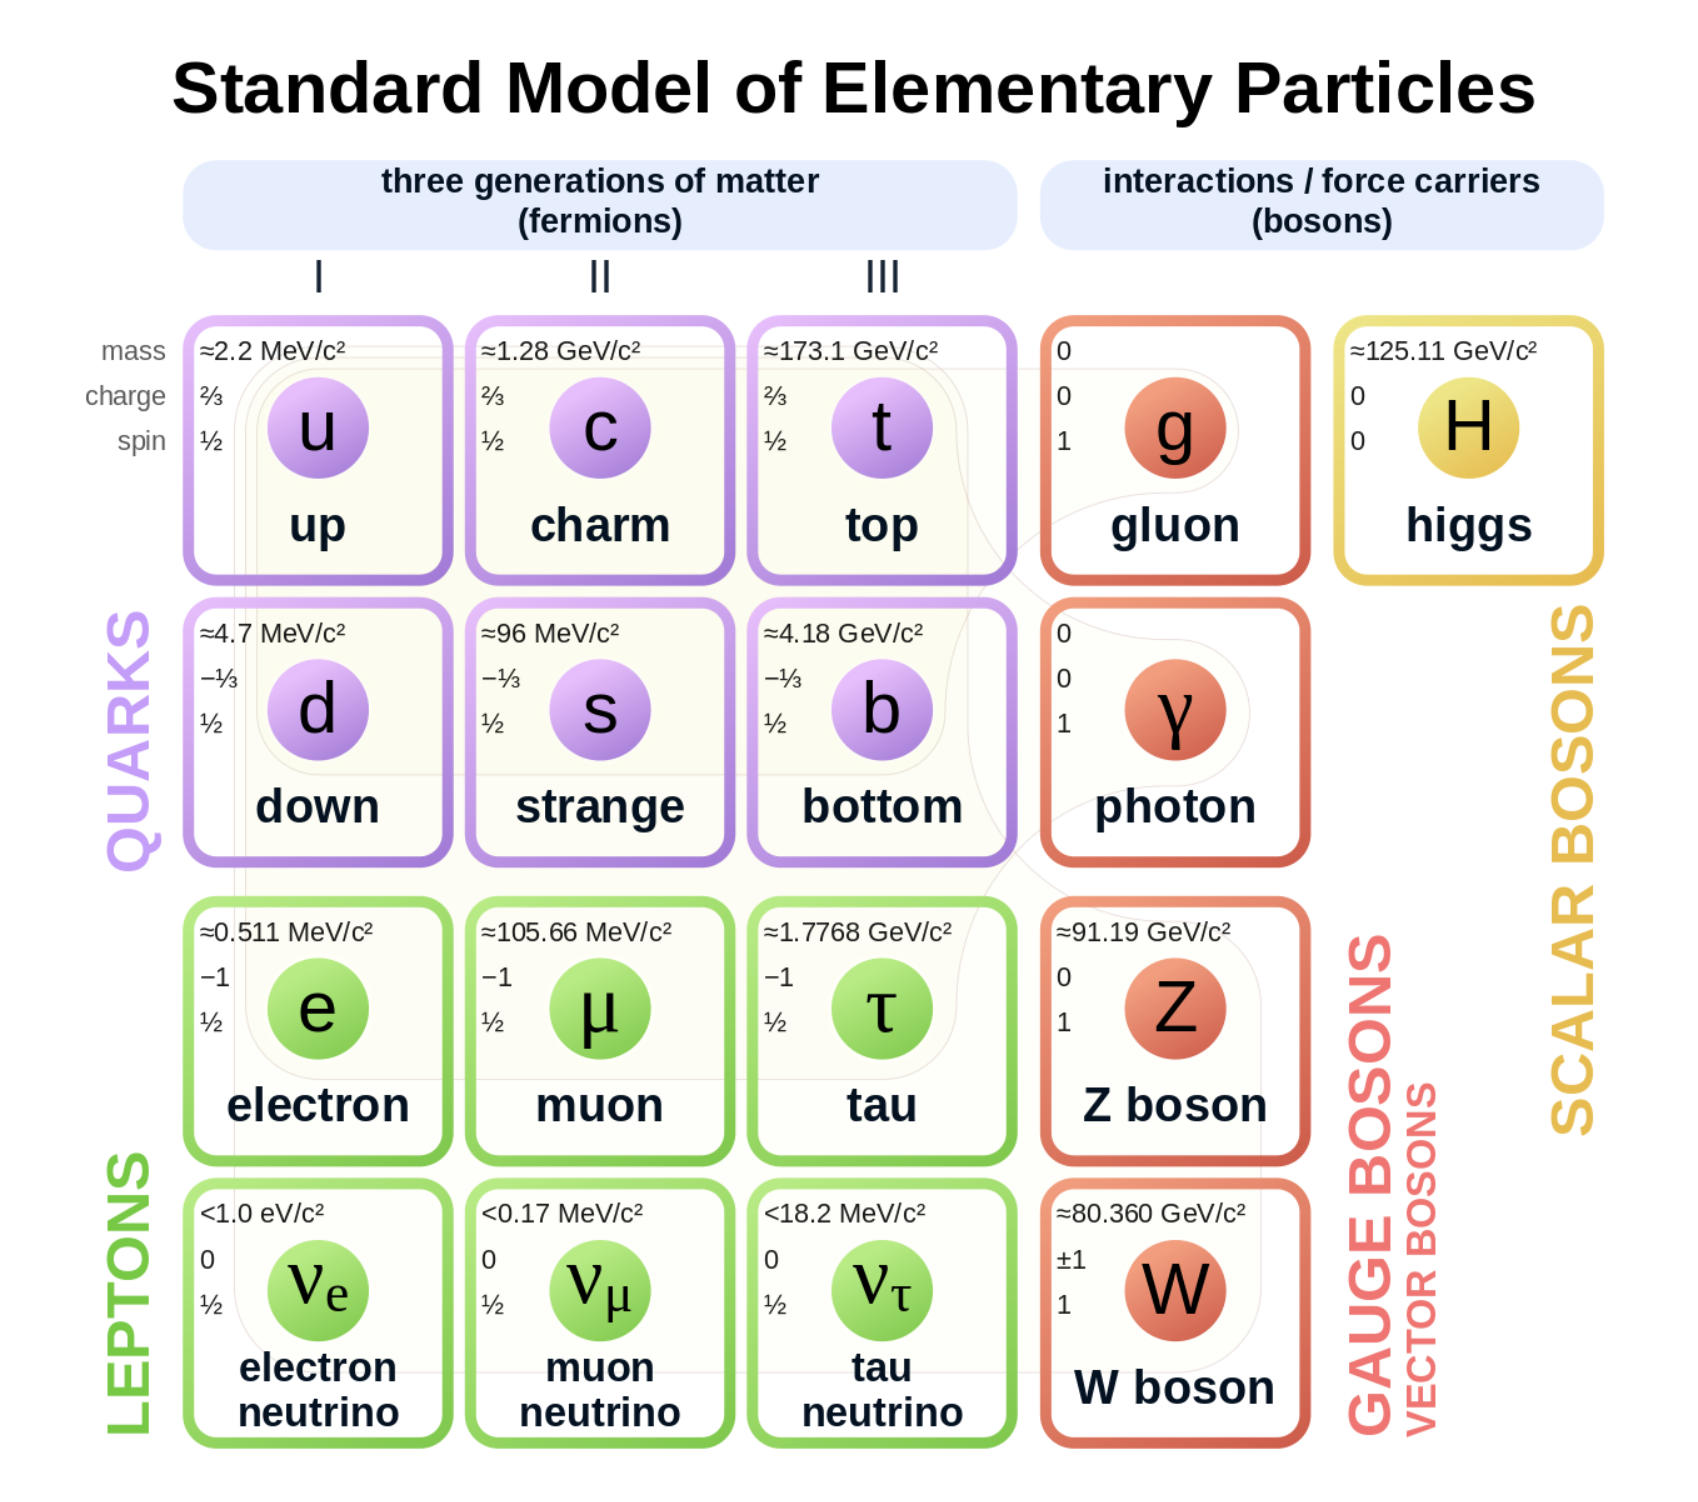
\includegraphics[width=0.7\textwidth]{figures/ch1/standard_model.png}
	\caption{Diagram of the 17 particles comprising the Standard Model}
	\label{fig:sm}
\end{figure}

Each entry is accompanied by 3 characteristic numbers: mass, charge, and spin. The mass of each particle is determined to limited precision by experimental observation, with the exception of photons and gluons which are known to be massless. Charge refers to the familiar electromagnetic charge in the case of leptons, W and Z bosons, and to color charge in the case of quarks and gluons. Spin is an intrinsic form of angular momentum carried by fundamental particles; all fermions have half integer spin, while bosons have integer spin. \par

Fermions come in flavor families
%flavors

Each particle is also known to have an \textit{antiparticle}. Each antiparticle has the same mass but the opposite charge of their Standard Model counter part; for example, the antiparticle of the electron is the positron, which has all the same properties but a positive charge. The photon, Z boson, and Higgs are all their own antiparticle. The nature of antineutrinos is an open question driving neutrino physics research, as it is not currently known whether neutrinos are their own antiparticle. \par

\subsection{Forces}
The three fundamental forces explained by the Standard Model are the electromagnetic force, the strong force, and the weak force. The photon is the carrier of the electromagnetic force, which dictates the nature of interactions between electrically charged particles, and is widely covered by introductory physics courses. The electromagnetic force has an infinite interaction range, a result of the massless and non-self interaction nature of the photon. The electromagnetic interaction is described by the theory of quantum electrodynamics (QED).\par

The weak force gives rise to atomic radiation and decay. It allows for the processes of beta decay and electron capture, which enable protons to convert to neutrons, and vice-versa, within the nucleus of an atom. In the process of beta decay, a proton decays into a neutron, a positron, and a neutrino; or, a neutron decays into a proton, an electron and an antineutrino. The weak interaction also plays a roll in the processes of nuclear fusion and nuclear fission. The  W\textsuperscript{+}, W\textsuperscript{-}, and Z\textsuperscript{0} are the force carriers of the weak force. The effective range of the weak force is limited to subatomic distances, as a result of the massive nature of the mediator bosons. The unified theory of the electroweak interaction posits that at high enough energies the electromagnetic interaction and the weak force merge into the same force. This threshold is termed the unification energy and estimated to be around 246 GeV. \par

The strong force confines quarks into hadron particles, such as protons and neutrons. The strong force also allows for the creation of atomic nuclei by binding protons and neutrons together, and is generally referred to as the ``nuclear force" in this context. The gluon is the mediator of the strong force, which is a short-range force which acts at subatomic distances on the order of $10^{-15}$ m. At this range, the strong force is about 100x as strong as the electromagnetic force, which allows for the creation of positively charged nuclei \cite{griffths}. The strong force is described by the theory of quantum chromodynamics (QCD). In the same way that QED dictates the interaction of electrically charges particles, QCD dictates the interactions of \textit{color-charged} particles. Due to the particular importance of QCD in this thesis, this topic will be explored in detail in section \ref{sec:QCD}. \par

The fundamental Feynmann diagram for each of the three forces discussed here is depicted in Figure \ref{fig:force_feynmann}. The fourth fundamental force, gravity, is not currently explained by any known mechanism within the Standard Model. 

 \begin{figure}
     \centering
     \begin{subfigure}[b]{0.43\textwidth}
         \centering
         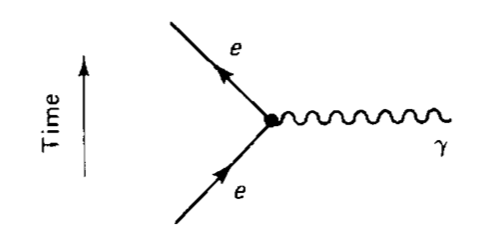
\includegraphics[width=\textwidth]{figures/ch1/em_force.png}
         \caption{The electromagnetic force}
     \end{subfigure}
     \hfill  
     \begin{subfigure}[b]{0.4\textwidth}
         \centering
         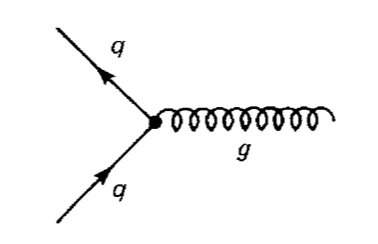
\includegraphics[width=\textwidth]{figures/ch1/strong_force.png}
         \caption{The strong force}
     \end{subfigure} \\
     \hfill
     \begin{subfigure}[b]{0.4\textwidth}
         \centering
         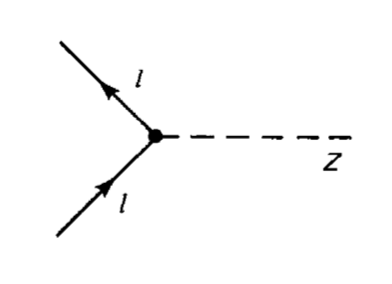
\includegraphics[width=\textwidth]{figures/ch1/weak_neutral.png}
         \caption{The neutral weak force}
     \end{subfigure}
     \hfill  
     \begin{subfigure}[b]{0.4\textwidth}
         \centering
         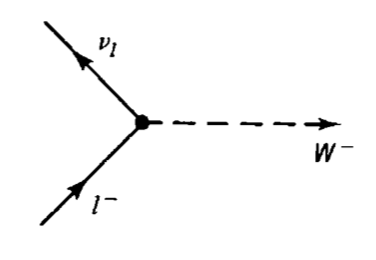
\includegraphics[width=\textwidth]{figures/ch1/weak_charged.png}
         \caption{The charged weak force}
     \end{subfigure} 
     \caption{Fundamental interactions of the three fundamental forces described by the Standard Model \cite{griffiths}. }
     \label{fig:force_feynmann}
\end{figure}

\section{QCD and Jets}
\label{sec:QCD}
The role of color in QCD at the surface level is analogous to that of electric charge in QED. However, while there is only one type of electric charge, there are three types of color charge - red, green, and blue. In the process $q \rightarrow q+g$, the color of the quark can change. In order to conserve color charge, gluons are bicolored, and always carry positive color charge and negative color charge. \par
Color charged particles only exist in bound states which result in a neutral total color charge, a principle known as confinement. This requires that quarks and gluons exist in group states known as hadrons; either mesons in the case of two quarks or baryons in the case of three quarks. When a quark is separated from a hadron, confinement dictates that other colored objects are produced around the quark to obey confinement. An example of this process is shown in Figure \ref{fig:jet_feynmann}. This ensemble of objects, generally a mixture of quarks and gluons, is termed a \textit{jet}. Jets are among the most common phenomenon observed by particle detectors at hadron colliders.

\begin{figure}
	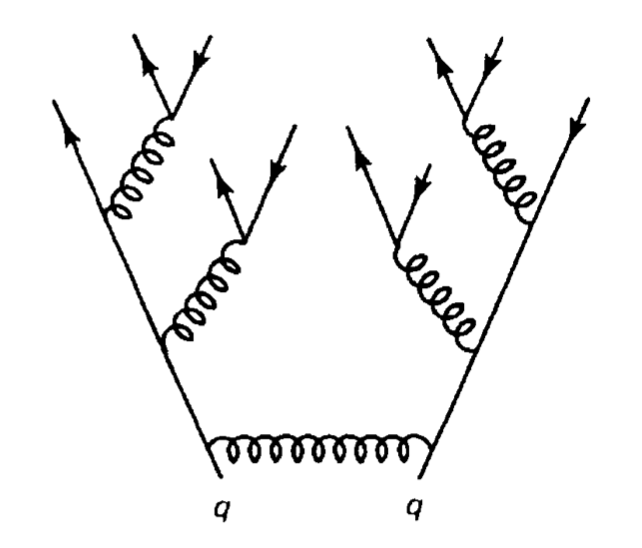
\includegraphics[width=0.5\textwidth]{figures/ch1/jet_feynmann.png}
	\caption{An example Feynmann diagram of jet production}
	\label{fig:jet_feynmann}
\end{figure}

\section{Symmetries}

The Standard Model is a renormalizable quantum field theory that obeys the local symmetry $G_{SM}$:

\begin{equation}
	G_{SM} = SU(3)_C \cross SU(2)_L \cross U(1)_Y .
\end{equation}

The $SU(3)_C$ symmetry component represents the non-Abelian gauge group of QCD. There are 8 generators for the $SU_C (3)$ group which correspond to the 8 types of gluon \cite{pdg}. \par

The $SU(2)_L \cross U(1)_Y$ symmetry group represents the electroweak sector of the Standard Model, which can be spontaneously broken into the electromagnetic and weak sectors. There are 4 generators for this group, which correspond to the four massless gauge bosons $W^1$, $W^2$, $W^3$, and B. From these massless gauge bosons are formed the massive mediators of the weak force, the $W^-$, $W^+$ and $Z^0$ bosons, and the massless electromagnetic force carrier, the photon $\gamma$. \par

Noether's theorem stipulates that any continuous symmetry is associated with a conserved quantity. In the Standard Model, this means that the $SU(3)_C$ symmetry gives rise to conservation of color charge. The $SU(2)_L \cross U(1)_Y$ symmetry gives rise to conservation of electromagnetic charge via symmetry breaking, which will be discussed in greater detail below. Conservation of spin results from the Poincar\'e symmetry described by the theory of special relativity, which combined with Noether's theorem gives us the conversation of energy, momentum, and angular momentum.\par

The SM Lagrangian is invariant under $CPT$ symmetry, or charge, parity, and time reversal. Charge conjugation ($C$) transform a particles into it's corresponding antipaticle by reversing the charge and other quantum numbers. Parity conjugation ($P$) reverses spatial coordinates, which transforms left-handed particles into right-handed particles and vice-versa. Time reversal ($T$) is the theoretical process of reversing time. The $L$ subscript in the $SU(2)_L$ group indicates that this symmetry only applies to the left-handed components of fermions. As a result, the $W^{1,2,3}$ generator bosons of $SU(2)_L$ only interact with left handed particles, a process which violates CP symmetry. The CPT theorem states that the violation of CP symmetry implies that T-symmetry must also be violated, so that $CPT$ is a preserved symmetry.

\subsection{Spontaneous Symmetry Breaking}
Higgs field a scalar field that forms a complex doublet of SU(2) 

Spontaneous symmetry breaking is the process by which a Lagranian obeys a symmetry at high energies, but exhibits asymmetric behavior at lower energies. The electroweak symmetry group is spontaneously broken as $SU(2)_L \cross U(1)_Y \rightarrow U(1)_{EM}$. The quantity conserved by the $SU(2)_L$ symmetry is weak isospin $T_{1,2,3}$, while the quantity conserved by $U(1)_Y$ symmetry is weak hypercharge $Y$. Below very high energies, the presence of the Higgs field causes the electroweak symmetry to break. This causes the four massless gauge bosons ($W^{1,2,3}$ and $B$) to mix, resulting in the massive gauge bosons $W^-$, $W^+$ and $Z^0$ bosons and the massless photon $\gamma$. The Higgs mechanism allows the $W^\pm$ and $Z$ bosons to be massive. The symmetry breaking also violates the conservation of weak isospin and weak hyperchage, leaving only electromagnetic charge $Q = T_3 + \frac{1}{2}Y$ as a conserved quantity associated with the $U(1)_{EM}$ symmetry. \par


\section{Experimental Validation of the Standard Model}
TODO: add citations for all original discoveries.\\

The theoretical framework of the Standard Model coalesced into a unified theory in the mid-20th century. A cascade of discoveries providing empirical evidence for the model followed closely. In the 1960s, three quarks (up, down and strange) and four leptons (electron, muon, and their associated neutrinos) were the known particulate building blocks of matter and the Standard Model. The discovery of the charm quark in 1974, through the observation of the $J/\psi$ meson \cite{SLAC_J}\cite{BNL_J}, confirmed the existence of a fourth quark flavor and explained the absence of flavor-changing neutral currents \cite{griffiths}. The discovery of the $\tau$ in 1975 \cite{tau} provided the first evidence of a 3rd generation of matter. This was quickly followed by the observation of the $\Upsilon$ meson in 1977, which provided evidence for the existence of a fifth quark, the $b$ bottom quark (sometimes also referred to as the beauty quark). The existence of a 3rd generation of fermion also explained the observation of CP violation in the weak force, as it allows for the appearance of a complex phase in the CKM matrix. The $t$ top quark and $\nu_\tau$ tau neutrino were predicted at this point as the final building blocks of three complete generations of fermions, and they were discovered by experimental observation around the turn of the 21st century. \par

The W and Z bosons were predicted by the Standard Model, but to observe them required the construction of a particle accelerator powerful enough to produce them. They were finally observed at CERN in 1983 by the UA1 and UA2 experiments at the newly constructed Super Proton Synchrotron (SPS). Their masses were observed to be compatible with those predicted by the Standard Model nearly a decade earlier. The final missing piece then was confirming the existence of the Higgs, which again required the construction of a newer and more powerful collider. CERN achieved this with the construction of the Large Hadron Collider (LHC), and in 2012 the ATLAS and CMS experiments announced the discovery of the Higgs particle. 

\section{Limitations of the Standard Model}
\label{sec:lim_sm}
TODO: add citations for all phenomenon.\\

While the Standard Model has enjoyed decades of experimental results which confirm its predictions, there are several glaring shortcomings. The observed phenomenon for which the Standard Model provides no explanation are summarized below.

\begin{itemize}
  \item Gravity - the Standard Model does not account for the fourth fundamental force of gravity.
  \item Dark Matter - there is no viable candidate to explain the existence of dark matter, a non-interacting form of matter which must exist to account for gravitational observations which cannot be explained by general relativity, such as the motion of galaxies, gravitational lensing, and the structure of the universe.
  \item Matter-Antimatter asymmetry - the level of CP violation in the Standard Model isn't sufficient to explain the large discrepancy between the amount of matter and the amount of antimatter in the universe today, and the origins of this imbalance are not understood.
  \item Neutrino masses - the Standard Model assumes that neutrinos are massless and provides no mechanism for them to acquire mass. However, observations of neutrino oscillations indicates they posses some very small but non-zero mass.
\end{itemize}

In additional to these unexplained natural phenomenon, there are several questions about the \textit{naturalness} of the Standard Model. The principle of naturalness states that dimensionless ratios between physical constants should be of order 1, and that nature should not be arbitrarily fine-tuned. While this is largely an aesthetic argument, it points to many aspects of the Standard Model for which there exists no natural explanation.

\begin{itemize}
  \item Strong CP - while CP symmetry is violated in the weak force, it appears to be preserved in the strong force, although CP violation in the strong force is allowed by the SM. There is no principle which motivates this incongruity between the weak force and strong force.
  \item Hierarchy Problem - The wide range of masses for elementary particles and the wide range of scales at which the four fundamental forces operate is not motivated by the SM. Specifically, it is not understood why the Higgs mass is observed to be well below the Plank scale $\lambda$, which is the energy level at which the effects of quantum gravity become significant. QFT indicates that the Higgs mass is determined by contributions from all energy scales including $\lambda$, which indicates that it's observed mass is inexplicably small.
\end{itemize}

These limitations of the Standard Model provide a road map for theoretical and experimental particle physicists, who seek to develop new theories which account for these observations, and then to find evidence which might support these \textit{beyond the Standard Model} (BSM) theories. The next chapter will introduce the BSM theories which motivate the physics search presented in this thesis. 
  
\chapter{Physics Beyond the Standard Model}
\section{Hidden Valley Theories}
\section{Semi-visible Jets}

%%%%%%%%%%%%%%%%
% Chapter 2
%%%%%%%%%%%%%%%%
\chapter{Physics Beyond the Standard Model}
In light of the various phenomenon unexplained by the Standard Model, physicists have proposed various extensions to the Standard Model, collectively termed \textit{Beyond the Standard Model} (BSM) theories. 
A particular focus of the physic programs at the Large Hadron Collider (LHC) are BSM models which suggest dark matter candidate particles. If these particles couple to Standard Model, they could be produced and observed at the LHC.

\section{Hidden Valley Models}
\label{sec:hiddenvalley}

Hidden Valley (HV) models are a category of BSM models that allow for dark matter (DM) production at the LHC. They extend the Standard Model with an additional non-Abelian gauge group \cite{snowmass}. This introduces the possibility of a complex dark sector, which mirrors the complexities of Standard Model QCD, and introduces the possibility of dark quarks and gluons. The term ``hidden valley" refers to the idea that the DM is hidden from the SM by a high-energy barrier, as illustrated in Figure \ref{fig:ch2/hidden_valley_sketch.png}. The dark sector is assumed to communicate with the Standard Model via a ``portal", or ``messenger particle", that can interact with both Standard Model and HV forces. For the s-channel scenario, the portal is considered to be a new massive mediator particle Z' . \par

\begin{figure}[h]
        \centering
	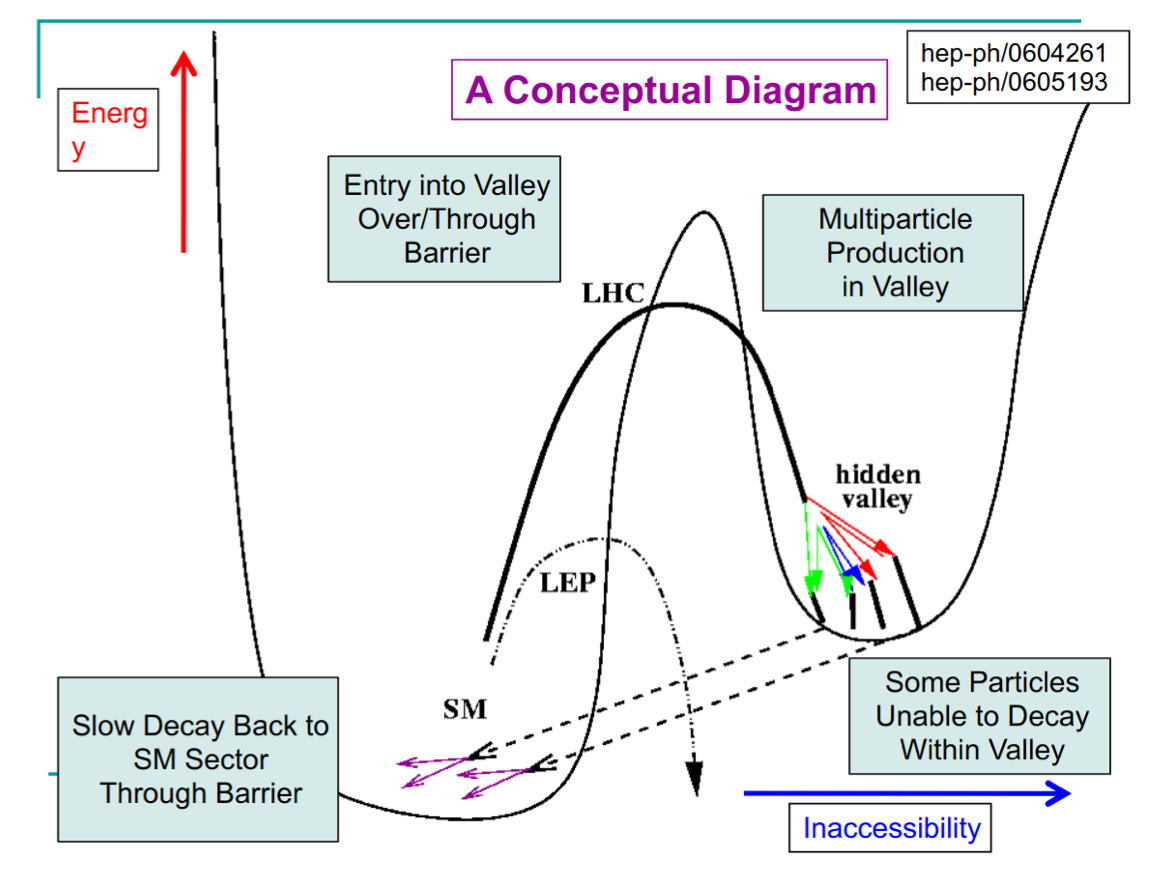
\includegraphics[width=.5\textwidth]{figures/ch2/hidden_valley_sketch.png}
        \label{fig:ch2/hidden_valley_sketch.png}
         \caption{Illustration of the hidden valley potential}
\end{figure}

The portal particle allows for the production of dark sector particles at hadron colliders. If dark quarks are produced via the decay $Z' \rightarrow q_D q_D$ they can hadronize and form dark jets. The properties of the dark jets are determined by the dynamics of the dark sector, which are explored in the subsequent section. Depending on the details of the model, the jets formed by the dark hadrons can be categorized as fully dark, semi-visible, leptonic, emerging, or other \cite{snowmass}. \par

\begin{figure}[h]
        \centering
	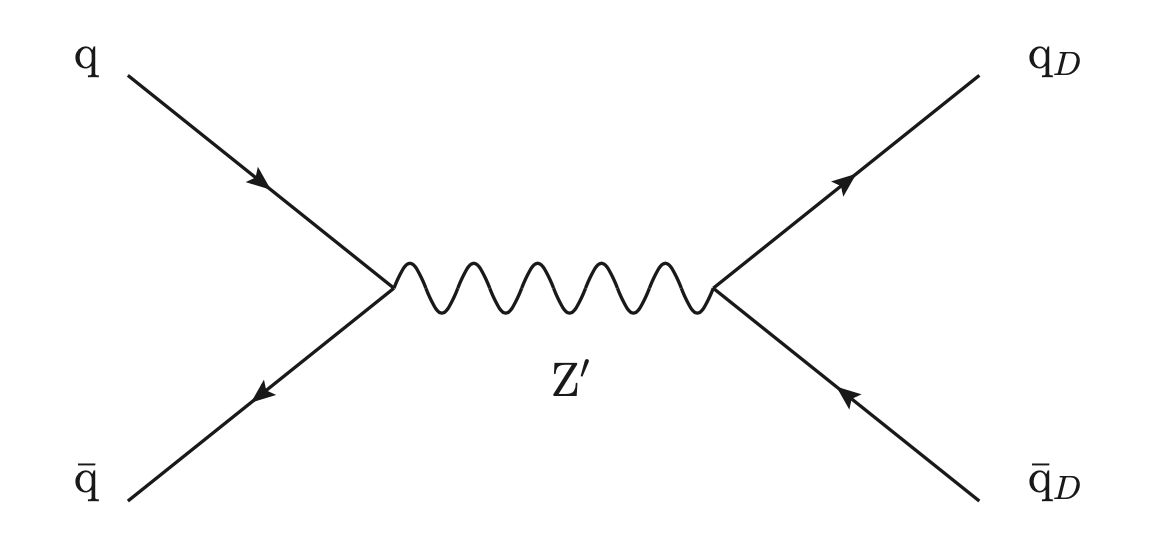
\includegraphics[width=.5\textwidth]{figures/ch2/zprime_feynman_diagram.png}
        \label{fig:ch2/zprime_feynman_diagram.png}
        \caption{The massive mediator particle Z' of the s-channel realization of a HV model}
\end{figure}

\section{Dark QCD}
\label{sec:darkqcd}
The theoretical underpinning of the semi-visible jet phenomenology is a dark sector with a gauge group $SU(N_d)$ leading to confinement at a scale $\Lambda_d$. For illustration, let's consider the case of an $SU(2)_d$ gauge theory, which gives rise to two dark fermionic generations $\chi_a = \chi_1, \chi_2$. Following the work of Timothy Cohen, et.al. we can write the fundamental dark Lagrangian as:
\begin{equation}
	\mathcal{L}_{dark} \supset - \frac{1}{2} \Tr G^{d}_{\mu\nu} G^{d\mu\nu} - \bar{\chi_a} (i {D\mkern-11.5mu/}-M_{d,a}) \chi_a
\end{equation}

The first term allows for the dark gluons to self-interact, while the second term enables the dark quarks to hadronize and acquire mass. The dark quarks are assumed to have a common mass $M_d$. The coupling strength of the strongly interacting dark quarks is termed $\alpha_d$. At the confinement scale $\Lambda_d$, the dark quarks can form bound states. At the scale $M_d \approx \Lambda_d$ a QCD-like show occurs. \par 

The properties of the hadrons formed by the dark quarks are of particular importance to the observed dark QCD dynamics. Dark-isospin number $U(1)_{1-2}$ and dark-baryon number $U(1)_{1+2}$ are accidental symmetries of the theory which determine the stability of the hadrons. In the case of two dark flavors, six dark hadrons can be formed: four mesons ($\chi_1\bar{\chi_1}$, $\chi_2\bar{\chi_2}$, $\chi_1\bar{\chi_2}$, $\bar{\chi_1}\chi_2$) and two baryons ($\bar{\chi_1}\bar{\chi_2}$, $\bar{\chi_1}\bar{\chi_2}$). The mesons $\chi_1\bar{\chi_2}$ and $\bar{\chi_1}\chi_2$ are charged under dark-isospin and will be stable if this symmetry is unbroken. The baryons would also be stable as they are charged under the dark-baryon number. These four stable hadrons become dark matter candidates of the theory. The $\chi_1\bar{\chi_1}$ and $\chi_2\bar{\chi_2}$ mesons are not charged under either symmetry and are thus expected to decay. The unstable mesons can decay into stable dark mesons, or into an off-shell Z'. The off-shell Z' will then decay into two DM quarks or two SM quarks, and it's products will continue to shower until the final state particles are stable.\par

The number of stable and unstable dark states varies substantially depending on the details of the model. The model discussed above can be generalized from $SU(2)_d$ to $SU(N)_d$, with any number of colors $N_c$ or flavors $N_f$. This affects the ratio of possible stable to unstable mesons, which can directly impact the amount of missing energy. The fraction of missing energy is a variable in many dark QCD models, and is especially important in the case of semi-visible jets.

\section{Semi-visible Jets}
\label{sec:semivisiblejets}

A ``semi-visible jet" occurs when the heavy Z' messenger particle decays into dark quarks, which then hadronize in a QCD-like shower. If some of the dark hadrons are stable while others decay to SM quarks via the off-shell Z', a collimated mixture of visible and dark matter is formed – this is termed a semi-visible jet. If the Z' messenger particle is produced at rest, the two jets will be back-to-back in the transverse plane. If there is an imbalance in the amount of invisible particles between the two jets, one of the jets will be observed to be aligned with missing transverse energy. \par

While there are a myriad of HV and dark QCD models, a handful of model parameters are most important in determining the observable of these showers within a particle detector. The coupling strength $\alpha_d$ is one of the most important, as it controls the fraction of dark hadrons emitted in the shower and their average \pt. The mass of the dark quarks directly impacts the jet mass. If the masses of the dark quark flavors are comparable, the ratio of stable to unstable dark hadrons will be approximately 1:1. However, if there is a mass splitting, stable or unstable dark hadrons may be favored, which impacts the amount of missing energy observed. \par

The ratio of stable to unstable dark hadrons in the shower is a critical variable for capturing the behavior of dark showers. This value is termed $r_{inv}$:
\begin{equation}
	r_{inv} = \frac{\textrm{\# of stable hadrons}}{\textrm{\# of hadronss}}
\end{equation}

Events containing jets aligned with missing transverse momentum are generally considered to be misreconstructed by other DM searches, and therefore discarded. This class of final states is therefore largely uncovered by existing DM searches. The nature of the dark hadron shower is determined by the following parameters: the Z' mass $m_{Z'}$, the Z' couplings to visible and dark quarks $g_q$ and $g_{q_D}$, the number of dark colors and flavors, the characteristic scale of the dark sector confinement $\Lambda_D$, the scale of the dark hadrons $m_D$, and the average fraction of stable hadrons in the decay $r_{inv}$. The coupling to SM quarks determines the Z' production cross section.



%%%%%%%%%%%%%%%%
% Part 2
%%%%%%%%%%%%%%%%
\part{Experiment}

%%%%%%%%%%%%%%%%
% Chapter 3
%%%%%%%%%%%%%%%%
\chapter{The Large Hadron Collider}
The Large Hadron Collider (LHC) is a 26.7 km circular high-energy particle accelerator, spanning the Swiss-French border near the city of Geneva, Switzerland \cite{LHC_machine}. The LHC occupies the tunnel constructed in 1989 for the Large Electron-Positron (LEP) Collider, and reaches a maximum depth of 170m below the surface. The LHC is operated by the European Organization for Nuclear Research (CERN), the largest international scientific collaboration in the world.\par

The LHC accelerates protons and heavy ions, and collides them at four interaction points around the ring, with a design center-of-mass energy per collision of $\sqrt{s}$ = 14 TeV. Each interaction point is home to one of four detector experiments, which study the products of the collisions. The largest of these experiments is the ATLAS detector, a general purpose detector designed to study the Standard Model and search for new physics that could be produced in LHC collisions \cite{ATLAS_at_LHC}. The CMS detector is another general purpose detector, designed and operated independently of the ATLAS detector, but intended to probe the same range of physics \cite{CMS_at_LHC}. The ALICE experiment is a dedicated heavy ion experiment, and the LHC-b experiment is a dedicated $b$-physics experiment  \cite{ALICE_at_LHC} \cite{LHCb_at_LHC}.\par

This chapter will cover the multi-component accelerator complex powering the LHC, the state-of-the-art magnets which steer the particle beams, measurements of the intensity and number of collisions produced by the LHC, and finally an overview of LHC activities in the past, present, and future.

 \section{Accelerator Physics}
 \subsection{The Journey of a Proton}
 \label{sec:proton_journey}
From 2010 - 2018, the protons which fed the LHC started as hydrogen gas. The electrons were removed from the hydrogen atoms through the use of strong electric fields. The linear accelerator LINAC2 then accelerated the protons to an energy of 50 MeV. Between 2018 and 2020, LINAC2 was replaced with LINAC4, which instead accelerates $H^{-}$ ions, hydrogen atoms with two electrons. LINAC4 is capable of accelerating the $H^-$ ions to 160 MeV. Before injection to the next part of the acceleration chain, both electrons are stripped from the $H^-$ ions, leaving just protons. From here the protons enter the Proton Synchrotron booster, where they are accelerated up to 1.4 GeV of energy. Subsequently they are sorted into bunches separated in time by 25 ns, where each bunch contains approximately $10^{11}$ protons. Next the bunches pass through the Proton Synchrotron (PS) and the Super Proton Synchrotron (SPS), where they reach energies of 25 GeV and 450 GeV respectively. Finally they are injected into the LHC as two beams traveling in opposite direction. The original design allowed each beam to be accelerated up to 7 TeV of energy. Due to limitations in the performance of the superconducting LHC magnets, the highest energy actually achieved by the LHC beams during Run 2 was 6.5 TeV, giving a collision center-of-mass energy of $\sqrt{s}$ = 13 TeV \cite{lhc_faq}. Figure \ref{fig:accelerator_complex} shows the full LHC accelerator complex.\par

\begin{figure}
	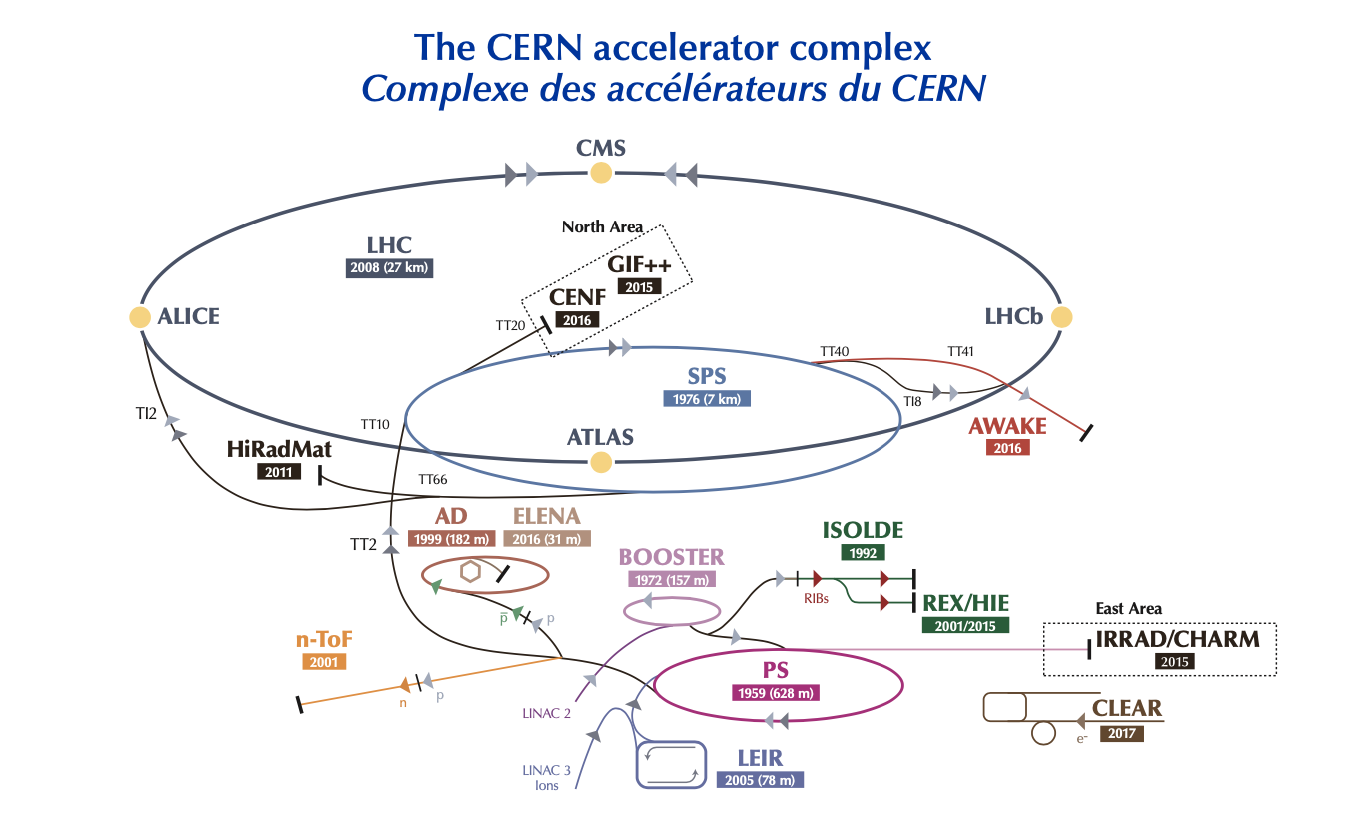
\includegraphics[width=\textwidth]{figures/ch3/accelerator_complex.png}
	\caption{The LHC accelerator complex at CERN \cite{cern_accelerator_complex}}
	\label{fig:accelerator_complex}
\end{figure}

 Acceleration in the LHC is performed by eight radio frequency (RF) cavities located around the ring. Each RF cavity produces a 2 MV electric field oscillating at 40 MHz. The 40MHz oscillation produces a point of stable equilibrium every 2.5 ns. These points of equilibrium are synchronized with the occurrence of the proton bunches produced in the PS -- a proton bunch occupies one out of every ten points of stable equilibrium, such that the bunches maintain a 25 ns spacing \cite{lhc_faq}. \\

\subsection{Magnets}
In addition to the acceleration cavities, the LHC houses 9593 superconducting magnets which direct and focus the proton beam on its 27 kilometer journey. The magnets are comprised of superconducting Niobium-Titanium coils cooled to 1.9K by superfluid helium. As the beams approach one of the four collision points around the ring, multipole magnets focus and squeeze the beam for optimal collisions \cite{lhc_faq}.\par

The LHC is divided into sections, where each section contains an a smoothly curving \textit{arc} and a straight \textit{insertion}. The arcs are composed of 1232 large dipole magnets which bend the beam to follow the roughly circular 27 km path. The main dipoles generate powerful 8.3 tesla magnetic fields to achieve this bend. Each dipole magnet is 15 meters long and weighs 35 tonnes. The dipoles work in conjunction with quadrupole magnets, which keep the particles in a focused beam, and smaller sextupole, octupole and decapole magnets which tune the magnetic field at the ends of the dipole magnets \cite{lhc_magnets}.\par

The straight insertion sections have different purposes depending on their location around the ring: beam collisions, beam injection, beam dumping, or beam cleaning. At the four collision points, insertion magnets squeeze the beam to ensure a highly focused collision. This is accomplished with a triplet of quadrupole magnets, which tighten the beam from 0.2 millimeters to just 16 micrometers in diameter. Insertion magnets also clean the beam, which prevents stray particles from hitting sensitive components throughout the LHC. When the LHC is ready to dispose of a beam of particles, beam dump magnets deflect the path of the beam into a straight line towards a block of concrete and graphite that stops the beam. A dilution magnet then reduces the beam intensity by a factor of 100,000 before the final stop \cite{lhc_magnets}. Figure \ref{fig:lhc_octants} shows the locations various beam activities.\par

\begin{figure}
        \centering
	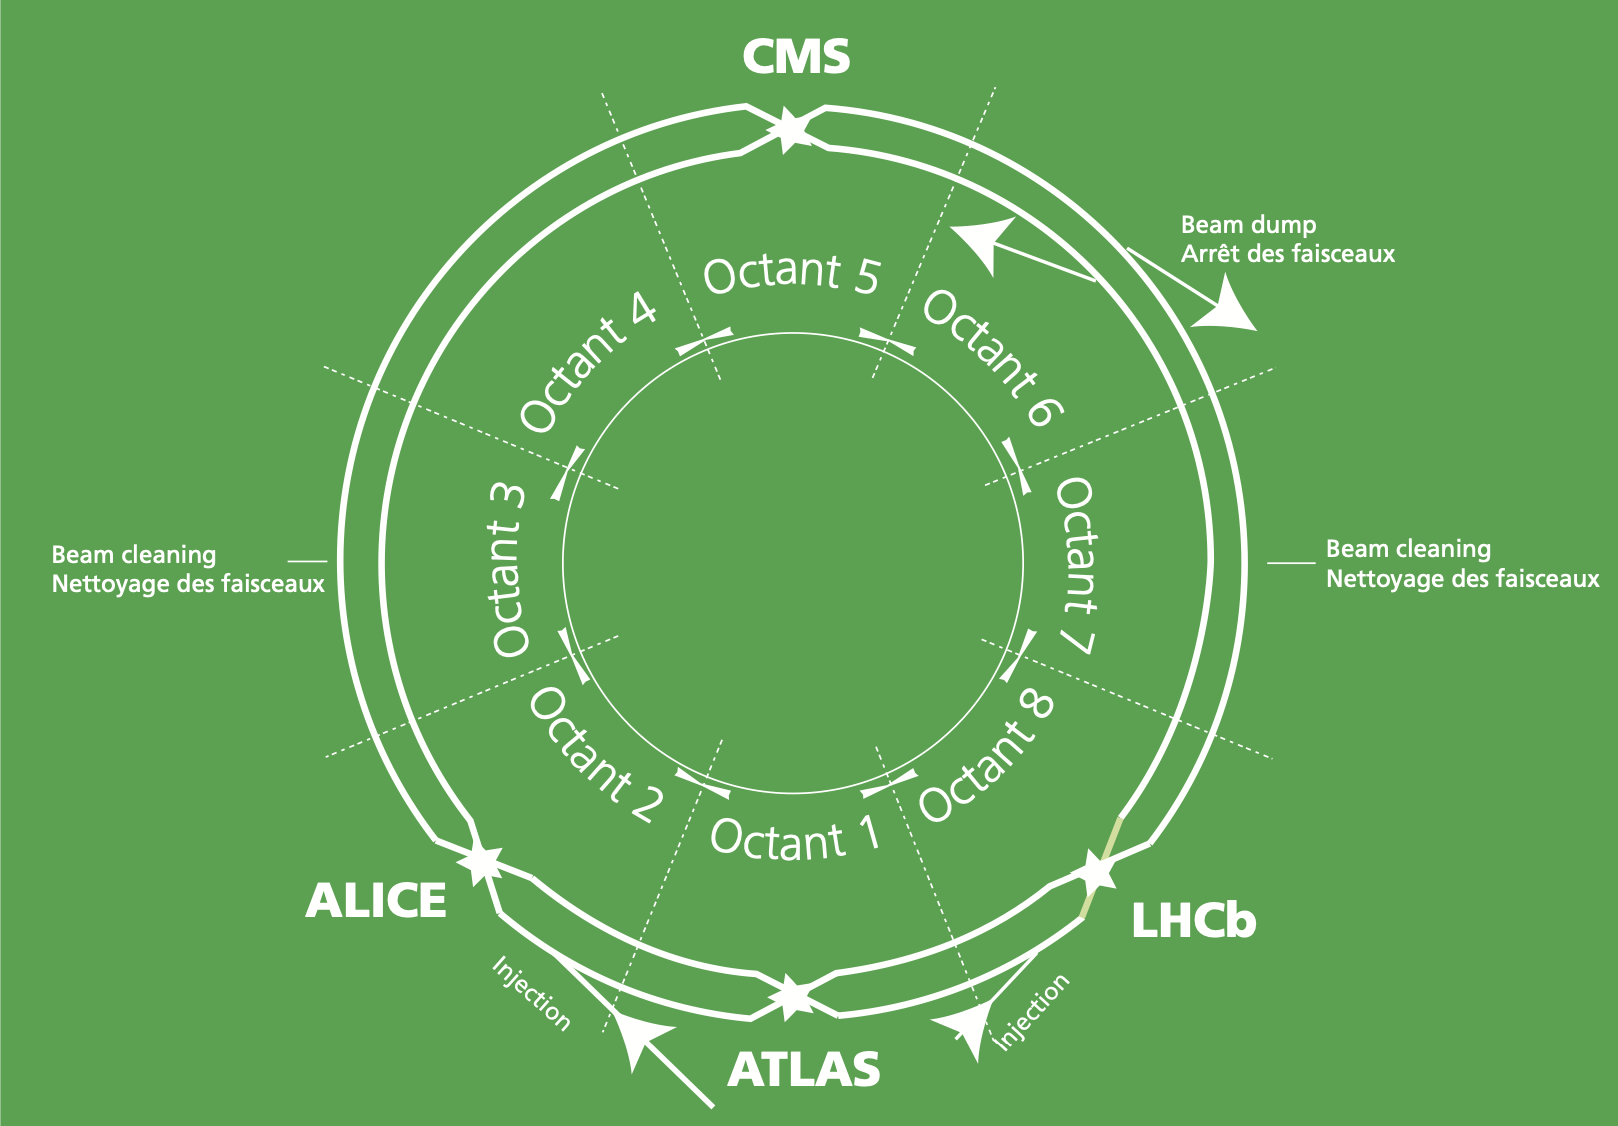
\includegraphics[width=.7\textwidth]{figures/ch3/lhc_octants.png}
	\caption{The octants of the LHC and location of various beam activities \cite{lhc_faq}. Stars indicate the locations of beam collisions, and the associated detectors recording the outcome of those collisions.}
	\label{fig:lhc_octants}
\end{figure} 
 
 \section{Luminosity}
 
Collisions at the LHC occur when the two beams of proton bunches cross at one of the four interaction points. The intensity of collisions is described by the instantaneous luminosity, the formula for which is given in equation \ref{eq:lumi}.  
 \begin{equation}
	L = \frac{f N_1 N_2}{4 \pi \sigma_x \sigma_y}
	\label{eq:lumi}
\end{equation}

Here $f$ is the revolution frequency, $N_1$ and $N_2$ are the number of particle per bunch for each beam, and $\sigma_x$, $\sigma_y$ are the horizontal and vertical beam widths. \par

The instantaneous luminosity gives the number of the collisions that could be produced at the interaction point per unit of cross-sectional area per unit of time, generally expressed in cm\textsuperscript{-2}s\textsuperscript{-1}. The integrated luminosity is obtained by integrating the instantaneous luminosity over a given block of time, and measures the total number of collisions which have occurred during that operation period. The total integrated luminosity is directly correlated with the size of the datasets collected by the LHC experiments. Total integrated luminosity for Run 2 is illustrated in Figure \ref{fig:lumi_run2}. \par 

High levels of instantaneous luminosity result in multiple $pp$ collisions per bunch crossing, which leads to an effect known as $pileup$. Pileup poses a challenge for detector physics, as reconstructing the products of multiple simultaneous events is far more challenging than reconstructing a single event with no pileup. Pileup conditions vary from year-to-year and run-to-run of LHC operation, and the impact of these conditions are taken into account when analyzing the data, as will be discussed further in Chapter \ref{ch:part_reco}. Measurement of pileup conditions during Run 2 are illustrated in Figure \ref{fig:lumi_run2}. \par
 
 \begin{figure}
     \centering
     \begin{subfigure}[b]{0.49\textwidth}
         \centering
         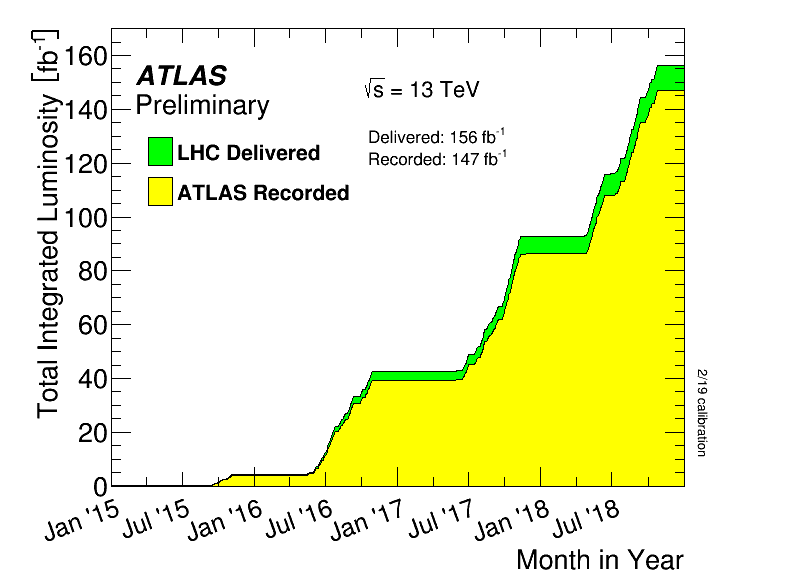
\includegraphics[width=\textwidth]{figures/ch3/lumi_integrated.png}
     \end{subfigure}
     \hfill  
     \begin{subfigure}[b]{0.48\textwidth}
         \centering
         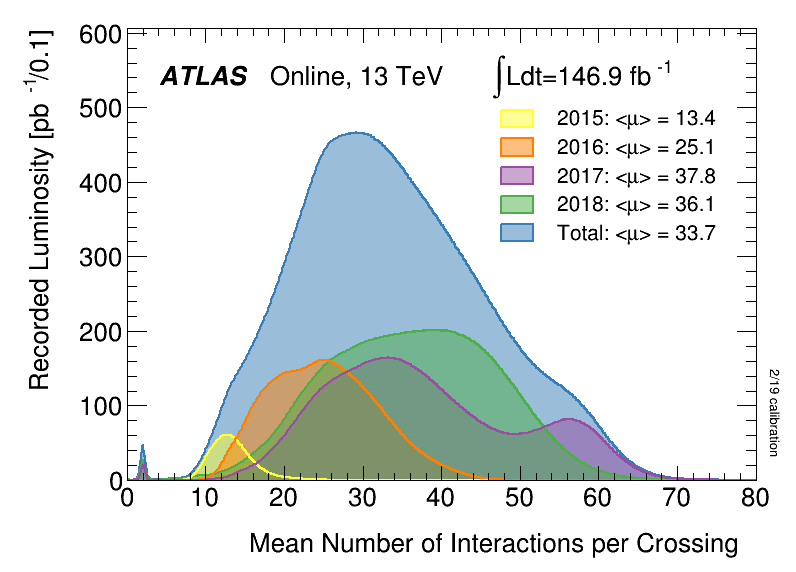
\includegraphics[width=\textwidth]{figures/ch3/lumi_instantaneous.png}
     \end{subfigure}
     \hfill
     \caption { (Left) Total integrated luminosity over the course of Run 2. (Right) Average number of $pp$ interactions per bunch crossing in Run 2. Each curve is weighted by the integrated luminosity for the year.}
     \label{fig:lumi_run2}
\end{figure}
 
 The design peak luminosity of the LHC is $1.0 \times 10^{34}$ cm\textsuperscript{-2}s\textsuperscript{-1}. During Run 1 of the LHC the peak instantaneous luminosity was $0.8 \times 10^{34}$ cm\textsuperscript{-2}s\textsuperscript{-1}. Over the course of Run 1 the LHC collected a total integrated luminosity of 5.46 \invfb at $\sqrt{s} = 7$ TeV, and 22.8 \invfb at $\sqrt{s} = 8$ TeV. Following the first long shutdown and upgrade phase of operations, the LHC achieved a center of mass energy $\sqrt{s} = 13$ TeV at the beginning of Run 2 in 2015. The LHC was also able to deliver $2.0 \times 10^{34}$ cm\textsuperscript{-2}s\textsuperscript{-1} peak instantaneous luminosity, double the design value. During LHC Run 2, from 2015-2018, the LHC delivered 156 \invfb of integrated luminosity for proton-proton collisions. Run 3 of the LHC began in 2022, and is expected to deliver $250$ \invfb of integrated luminosity to the ATLAS and CMS experiments by 2026 \cite{lhc_timeline}.\par
 
The goal of LHC physic analyses is to find and study rare events produced by interesting physics processes. The cross section $\sigma$ of a given process indicates the probability of that process occurring given the beam conditions of the LHC. Multiplying the cross section by the integrated luminosity of a dataset gives the expected number of events for that process within the dataset.

 \begin{equation}
	N\textsubscript{events} = \int \sigma L(t) dt = \mathcal{L} \times \sigma
	\label{eq:xs}
\end{equation}

The cross section for most processes of interest, especially BSM processes, is several orders of magnitude below the total cross section for the LHC. Therefore maximizing the number of events produced in collisions is crucial to increase the likelihood of producing events from processes of interest. For this reason, maximizing instantaneous luminosity is a key factor in accelerator design and operation, while mitigating the resulting pileup effects is a key component in detector design and operation. \par 

\section{LHC Timeline}
The first proton-proton collisions at the LHC were achieved in 2010 with a center-of-mass energy of $\sqrt{s}$ = 7 TeV. Run 1 of the LHC took place between 2010 and early 2013, during which time the center-of-mass collision energy increased from 7 TeV to 8 TeV. Figure \ref{fig:lhc_timeline} shows an overview of LHC activities beginning in 2011, in the midst of Run 1. The data collected during Run 1 led to the discovery of the Higgs boson in 2012 \cite{higgs_paper}. \par

Between 2013 and 2015 the LHC underwent the first Long Shutdown (LS1) during which time maintenance and renovation was performed on the accelerator chain, including the repair and consolidation of the high-current splices which connect the super-conducting LHC magnets. Run 2 of the LHC took place from 2015 to 2018 and achieved a center-of-mass energy of $\sqrt{s}$ = 13 TeV. Analysis of data collected in Run 2 is still on going, and is the subject of study in this thesis. \par

Between 2018 and 2022 the LHC underwent the second Long Shutdown (LS2), allowing for further detector and accelerator maintenance and upgrades. Key improvements to the LHC included the improvement of the insulation for over 1200 diode magnets, and the upgrade from LINAC2 to LINAC4 mentioned in Section \ref{sec:proton_journey}. Run 3 of the LHC began in 2022 and achieved a center-of-mass energy of $\sqrt{s}$ = 13.6 TeV. \par

Run 3 is scheduled to continue through 2026, at which point the LHC machine and detectors will undergo upgrades for the \textit{high luminosity} LHC (HL-LHC). The HL-LHC will increase the instantaneous machine luminosity by a factor of 5 - 7.5 with respect to the nominal LHC design. The bottom panel of Figure \ref{fig:lhc_timeline} shows an overview of the preparation work for the HL-LHC that has been going on concurrently with Run 1, 2, and 3 of the LHC \cite{hl_lhc}. 

\begin{figure}
        \centering
	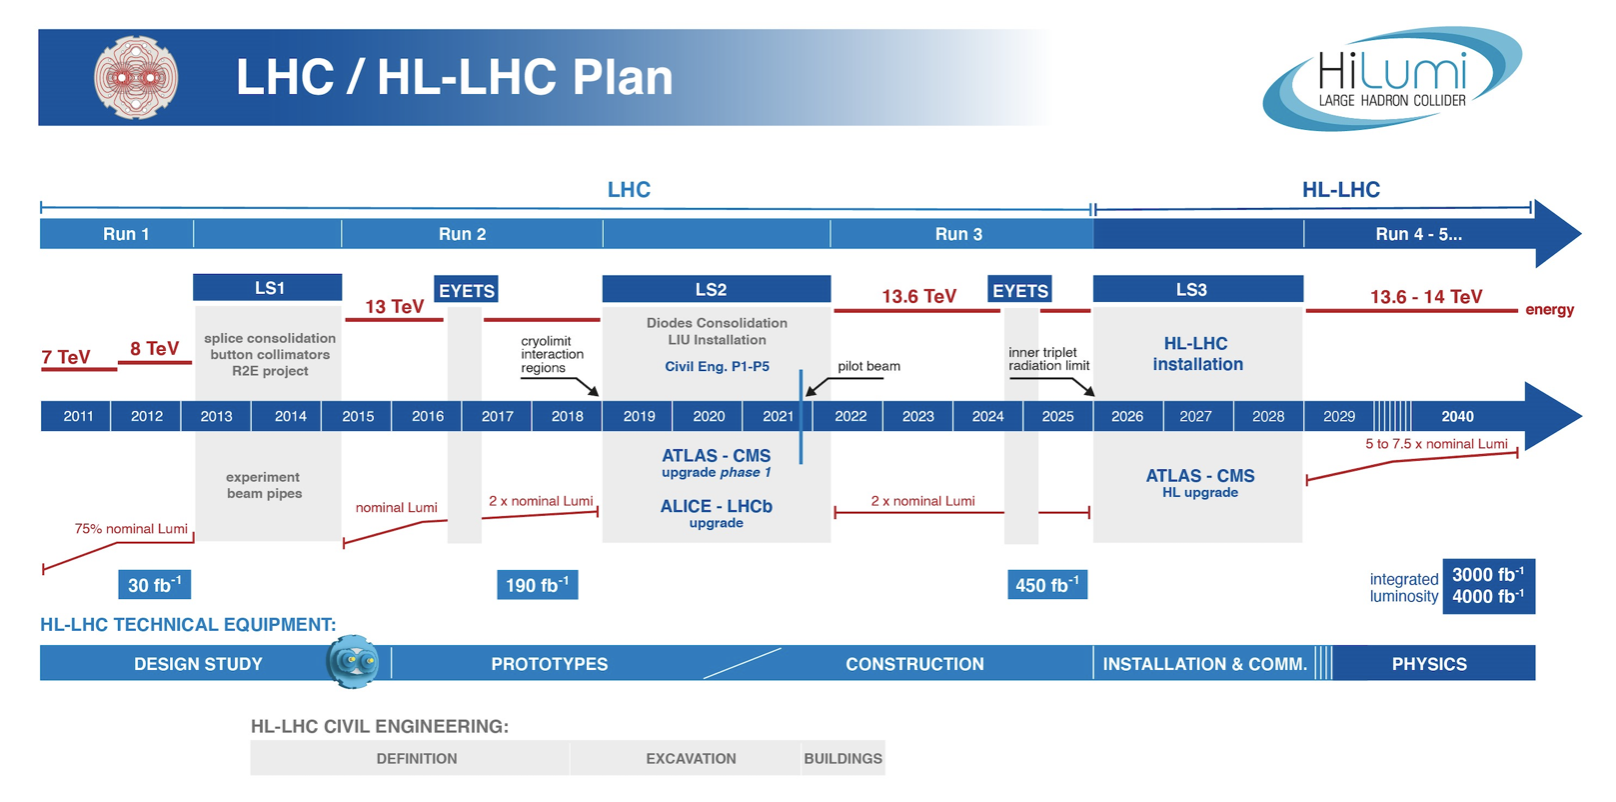
\includegraphics[width=0.9\textwidth]{figures/ch3/hl_lhc_timeline.png}
	\caption{Timeline of LHC and HL-LHC activities \cite{lhc_timeline}. Integrated luminosity estimates are approximate, and not reflective of the exact amount delivered to each experiment.}
	\label{fig:lhc_timeline}
\end{figure}


%%%%%%%%%%%%%%%%
% Chapter 4
%%%%%%%%%%%%%%%%
\chapter{Discussion}
Lorem ipsum dolor sit amet, consectetur adipiscing elit, sed do eiusmod tempor incididunt ut labore et dolore magna aliqua. Ut enim ad minim veniam, quis nostrud exercitation ullamco laboris nisi ut aliquip ex ea commodo consequat. Duis aute irure dolor in reprehenderit in voluptate velit esse cillum dolore eu fugiat nulla pariatur. Excepteur sint occaecat cupidatat non proident, sunt in culpa qui officia deserunt mollit anim id est laborum..
Lorem ipsum dolor sit amet, consectetur adipiscing elit, sed do eiusmod tempor incididunt ut labore et dolore magna aliqua. Ut enim ad minim veniam, quis nostrud exercitation ullamco laboris nisi ut aliquip ex ea commodo consequat. Duis aute irure dolor in reprehenderit in voluptate velit esse cillum dolore eu fugiat nulla pariatur. Excepteur sint occaecat cupidatat non proident, sunt in culpa qui officia deserunt mollit anim id est laborum..

Lorem ipsum dolor sit amet, consectetur adipiscing elit, sed do eiusmod tempor incididunt ut labore et dolore magna aliqua. Ut enim ad minim veniam, quis nostrud exercitation ullamco laboris nisi ut aliquip ex ea commodo consequat. Duis aute irure dolor in reprehenderit in voluptate velit esse cillum dolore eu fugiat nulla pariatur. Excepteur sint occaecat cupidatat non proident, sunt in culpa qui officia deserunt mollit anim id est laborum..

Lorem ipsum dolor sit amet, consectetur adipiscing elit, sed do eiusmod tempor incididunt ut labore et dolore magna aliqua. Ut enim ad minim veniam, quis nostrud exercitation ullamco laboris nisi ut aliquip ex ea commodo consequat. Duis aute irure dolor in reprehenderit in voluptate velit esse cillum dolore eu fugiat nulla pariatur. Excepteur sint occaecat cupidatat non proident, sunt in culpa qui officia deserunt mollit anim id est laborum..

Lorem ipsum dolor sit amet, consectetur adipiscing elit, sed do eiusmod tempor incididunt ut labore et dolore magna aliqua. Ut enim ad minim veniam, quis nostrud exercitation ullamco laboris nisi ut aliquip ex ea commodo consequat. Duis aute irure dolor in reprehenderit in voluptate velit esse cillum dolore eu fugiat nulla pariatur. Excepteur sint occaecat cupidatat non proident, sunt in culpa qui officia deserunt mollit anim id est laborum..

Lorem ipsum dolor sit amet, consectetur adipiscing elit, sed do eiusmod tempor incididunt ut labore et dolore magna aliqua. Ut enim ad minim veniam, quis nostrud exercitation ullamco laboris nisi ut aliquip ex ea commodo consequat. Duis aute irure dolor in reprehenderit in voluptate velit esse cillum dolore eu fugiat nulla pariatur. Excepteur sint occaecat cupidatat non proident, sunt in culpa qui officia deserunt mollit anim id est laborum..
Lorem ipsum dolor sit amet, consectetur adipiscing elit, sed do eiusmod tempor incididunt ut labore et dolore magna aliqua. Ut enim ad minim veniam, quis nostrud exercitation ullamco laboris nisi ut aliquip ex ea commodo consequat. Duis aute irure dolor in reprehenderit in voluptate velit esse cillum dolore eu fugiat nulla pariatur. Excepteur sint occaecat cupidatat non proident, sunt in culpa qui officia deserunt mollit anim id est laborum..
Lorem ipsum dolor sit amet, consectetur adipiscing elit, sed do eiusmod tempor incididunt ut labore et dolore magna aliqua. Ut enim ad minim veniam, quis nostrud exercitation ullamco laboris nisi ut aliquip ex ea commodo consequat. Duis aute irure dolor in reprehenderit in voluptate velit esse cillum dolore eu fugiat nulla pariatur. Excepteur sint occaecat cupidatat non proident, sunt in culpa qui officia deserunt mollit anim id est laborum..
Lorem ipsum dolor sit amet, consectetur adipiscing elit, sed do eiusmod tempor incididunt ut labore et dolore magna aliqua. Ut enim ad minim veniam, quis nostrud exercitation ullamco laboris nisi ut aliquip ex ea commodo consequat. Duis aute irure dolor in reprehenderit in voluptate velit esse cillum dolore eu fugiat nulla pariatur. Excepteur sint occaecat cupidatat non proident, sunt in culpa qui officia deserunt mollit anim id est laborum..
Lorem ipsum dolor sit amet, consectetur adipiscing elit, sed do eiusmod tempor incididunt ut labore et dolore magna aliqua. Ut enim ad minim veniam, quis nostrud exercitation ullamco laboris nisi ut aliquip ex ea commodo consequat. Duis aute irure dolor in reprehenderit in voluptate velit esse cillum dolore eu fugiat nulla pariatur. Excepteur sint occaecat cupidatat non proident, sunt in culpa qui officia deserunt mollit anim id est laborum..

Lorem ipsum dolor sit amet, consectetur adipiscing elit, sed do eiusmod tempor incididunt ut labore et dolore magna aliqua. Ut enim ad minim veniam, quis nostrud exercitation ullamco laboris nisi ut aliquip ex ea commodo consequat. Duis aute irure dolor in reprehenderit in voluptate velit esse cillum dolore eu fugiat nulla pariatur. Excepteur sint occaecat cupidatat non proident, sunt in culpa qui officia deserunt mollit anim id est laborum..
Lorem ipsum dolor sit amet, consectetur adipiscing elit, sed do eiusmod tempor incididunt ut labore et dolore magna aliqua. Ut enim ad minim veniam, quis nostrud exercitation ullamco laboris nisi ut aliquip ex ea commodo consequat. Duis aute irure dolor in reprehenderit in voluptate velit esse cillum dolore eu fugiat nulla pariatur. Excepteur sint occaecat cupidatat non proident, sunt in culpa qui officia deserunt mollit anim id est laborum..
Lorem ipsum dolor sit amet, consectetur adipiscing elit, sed do eiusmod tempor incididunt ut labore et dolore magna aliqua. Ut enim ad minim veniam, quis nostrud exercitation ullamco laboris nisi ut aliquip ex ea commodo consequat. Duis aute irure dolor in reprehenderit in voluptate velit esse cillum dolore eu fugiat nulla pariatur. Excepteur sint occaecat cupidatat non proident, sunt in culpa qui officia deserunt mollit anim id est laborum..



%%%%%%%%%%%%%%%%
% Chapter 5
%%%%%%%%%%%%%%%%
\chapter{Particle Reconstruction and Identification}
\label{ch:part_reco}

With a design luminosity of $1.0 \times 10^{34}$ cm\textsuperscript{-2}s\textsuperscript{-1}, and a peak Run-2 instantaneous luminosity of $2.0 \times 10^{34}$ cm\textsuperscript{-2}s\textsuperscript{-1}, reconstructing and identifying the products of LHC $pp$ collisions is one of the most complex tasks for each LHC experiment. The accurate reconstruction and identification of physics objects lays the ground work for all subsequent physics analyses, so it is also one of the most fundamentally important tasks performed by an experiment. \par

Reconstruction is the process of combining raw and uncalibrated hits across various subsystems into specific unique objects. Two particular subsystems, the Inner Detector (ID) tracker and the calorimeter play particularly important roles and will be discussed in detail. Analysis of the properties of the reconstructed objects identifies them as photon, electrons, muons, or jets. While photons, electrons, and muons are fundamental particles, jets represent a collimated shower of many hadronic particles, whose definition is more flexible. Jet reconstruction, clustering and substructure are all of particular important to jet identification, and to the later content of this thesis. Finally, reconstruction also identifies missing transverse energy \met in events, which is a crucial variable for BSM physics searches. Figure \ref{fig:detector_objects} shows how the various physics objects listed here interact with various systems in the ATLAS detector. 

\begin{figure}
        \centering
	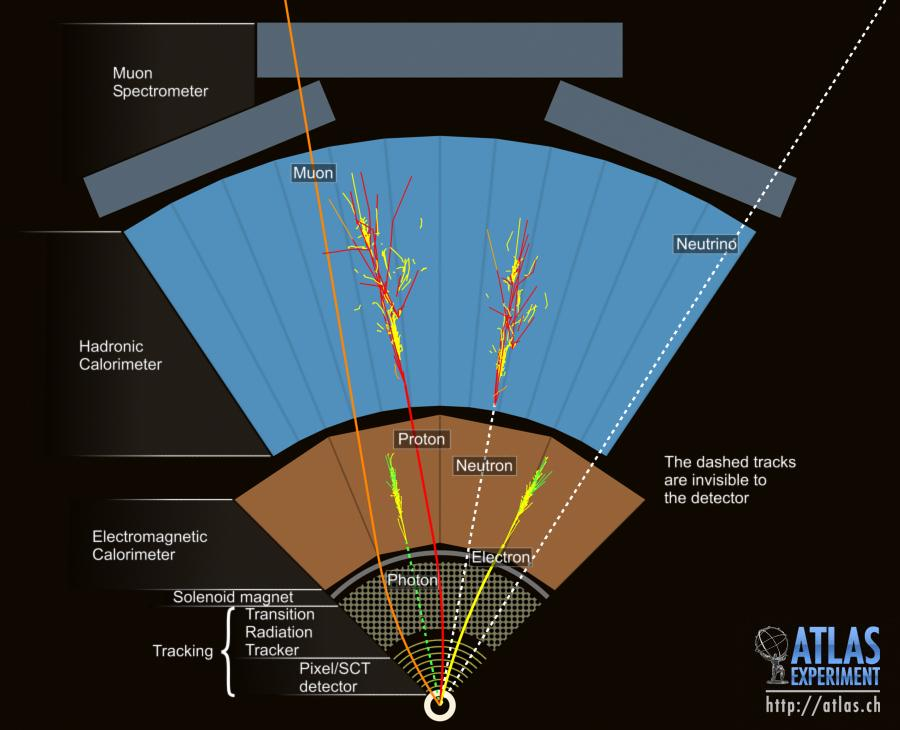
\includegraphics[width=0.8\textwidth]{figures/ch5/detector_objects}
	\caption{Graphic illustrating the various objects and high level features identified by ATLAS object reconstruction, and their interaction with different systems of the ATLAS detector \cite{detector_events}}
	\label{fig:detector_objects}
\end{figure}

\section{Inner Detector Tracks}
As the inner most layer of the detector, the ID measures charged particles close to the interaction point. The various hits of these charged particles throughout the ID are used to reconstruct \textit{tracks} which give the trajectories of charged particles. Track reconstruction begins by clustering hits in the Pixel and SCT detectors, and combining clusters from different radial laters of these detector. The multi-layer clusters form track \textit{seeds}, which provide initial estimates of measurements belonging to an individual track. The requirement of three points allows for a rough estimate of the track \pt to be made by calculating the curvature of the track and accounting of the magnetic field in the ID. \par

Tracks seeds are subject to a variety of quality requirements, such as having a minimum estimated \pt and passing interaction region compatability criterion. If these requirements are satisfied, the track seeds are passed to the track finding and fitting algorithms. The interplay of these three track reconstruction steps is illustrated in Figure \ref{fig:track_reco}. 

\begin{figure}
        \centering
	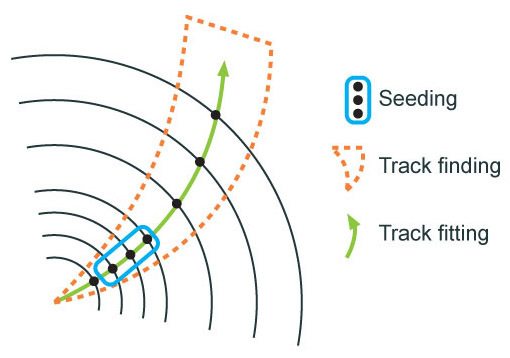
\includegraphics[width=0.6\textwidth]{figures/ch5/track_reco}
	\caption{Track reconstruction seeding, finding and fitting illustration \cite{track_finding}}
	\label{fig:track_reco}
\end{figure}


\section{Photons and Electrons}
\section{Muons}
\section{Jets}
\subsection{Calorimeter Clusters}
\subsection{Particle Flow Reconstruction}
\subsection{Jet Clustering}
\subsection{Jet Substructure}
\section{Missing Transverse Energy}


%%%%%%%%%%%%%%%%
% Part 3
%%%%%%%%%%%%%%%%
\part{Search}

%%%%%%%%%%%%%%%%
% Chapter 6
%%%%%%%%%%%%%%%%
\chapter{Monte Carlo and Data}
\label{ch:mc_data}

The search for semi-visible jets via s-channel production presented in the following chapters is performed with an integrated luminosity of 139 \fb~of proton-proton collision data collected by the ATLAS detector during Run 2 (2015 - 2018). The full Run 2 dataset is used for the final interpretation. Monte Carlo (MC) simulations of background processes and the semi-visible jet signal process are used in the development of the analysis strategy, and in the final interpretation to set limits on the observed cross-section of the signal model. This chapter will provide details about the full Run 2 dataset, and the background MC simulations, and the signal MC simulations used in this search. 

\section{Data}
The 139 \fb~integrated luminosity of proton-proton collision data used for physics analyses are required to pass a set of data quality checks. In Run 2 94\% of the $pp$ collisions delivered by the LHC were successfully recorded by the ATLAS experiment, as illustrated in Figure~\ref{fig:atlas_grl}. 95\% of the data recorded by the ATLAS experiment was marked as ``good for physics", resulting in 139 \fb~of integrated luminosity. Events are rejected if they are corrupted or incomplete, or if they were recorded during a subsystem malfunction. 

\begin{figure}
        \centering
	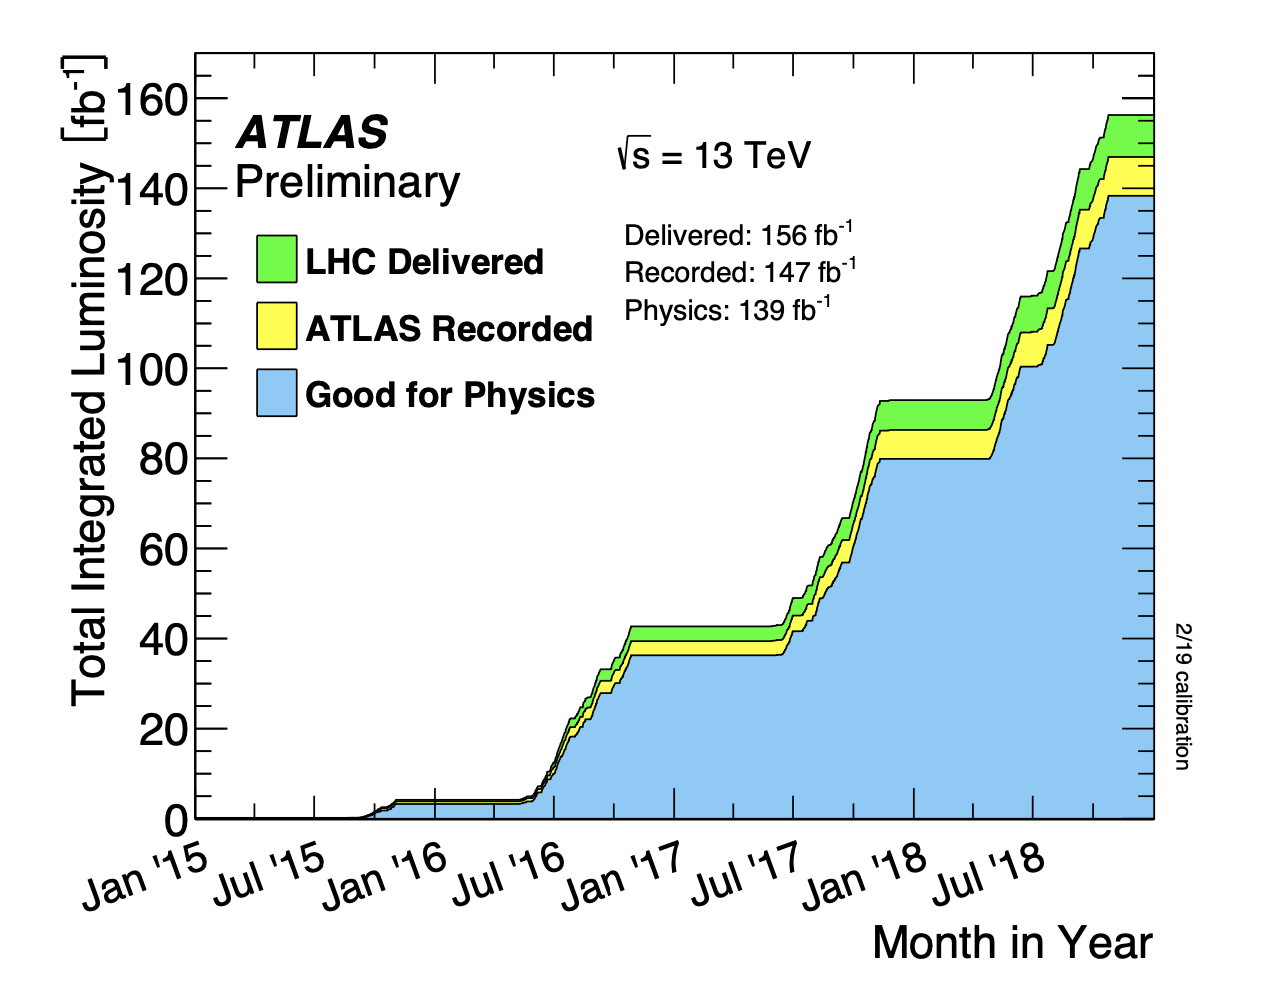
\includegraphics[width=0.62\textwidth]{figures/ch6/atlas_grl}
	\caption{Integrated luminosity for the ATLAS experiment as a function of time during Run 2 \cite{atlas_grl}
	\label{fig:atlas_grl}}
\end{figure}

Events for this analysis are further required to pass a single-jet trigger selection, where events are required to have at least one jet with a \pt~that exceeds a certain value. 
The lowest \pt~unprescaled\footnote{An unprescaled trigger records every event that meets the trigger requirement. A prescaled trigger only records a fraction of events that meet the trigger requirement.} single jet trigger threshold for each period is as follows: 

\begin{itemize}
\item 2015: \pt $\geq$ 360 GeV
\item 2016 \& 2017:  \pt $\geq$ 380 GeV
\item 2018:  \pt $\geq$ 420 GeV
\end{itemize}

A post-trigger selection of \textit{leading} jet \pt~> 450 GeV ensures these triggers are fully efficient, meaning that the jets are comfortably above the trigger threshold. The jet in the event with the highest \pt~is termed the \textit{leading jet} (or $j_1$), while the jet with the second highest \pt~is termed the \textit{subleading} jet (or $j_2$). The jet collection used is anti-$k_t$ EM particle flow jets with a radius parameter of R = 0.4, also referred to as small-R jets. \par

Due to the variance in visible and invisible momenta due to the \rinv~parameter of the signal model, many signals also have significant \met.
The use of a \met~trigger to select events was considered, and the single jet approach described here was found to preserve more signal events across the grid, particularly in the high resonance mass and low ~\rinv~region of phase space. These studies are documented in Appendix~\ref{app:trigger}.\par

The data are subject to a blinding strategy throughout the analysis design so as to mitigate analyzer-induced bias. 
Blinded and unblinded region definitions are described further in Section~\ref{sec:eventsel}.

\section{Simulation}
\label{sec:simulation}

Simulated events are generated with a variety of Monte Carlo (MC) generator processes that run in stages. The $pp$ hard scatter physics process is simulated, and the final state particles are subsequently showered and decayed. This full description of the event is then propagated through a detailed detector simulation based on GEANT4~\cite{Agostinelli:2002hh}. The MC simulation is weighted to match the distribution of the average number of interactions per bunch crossing $\mu$ observed in collision data.\par

All simulated samples included in this analysis were produced with three different MC campaigns: $\texttt{mc20a}$ corresponds to 2015-2016 data-taking conditions, $\texttt{mc20d}$ to 2017, and $\texttt{mc20e}$ to 2018. These three campaigns are weighted to the integrated luminosities of their respective data-taking periods and combined to produce simulation for the entire Run 2 dataset. Simulated events are reconstructed with the same algorithms run on collision data. 


\subsection{Simulated Backgrounds}
\label{subsec:bkg_mc}

Although the final background estimation is data-driven, background MC is studied for analysis optimization and machine learning tool development.\par

Dijet QCD is the dominant background process. QCD is simulated with \textsc{Pythia8}~\cite{pythia}, and generated in approximate slices of \pt, to ensure high statistics across the momentum spectrum. The slices are then reweighted using MC generated event weights to create a physical distribution. Figure~\ref{fig:jzslices} illustrates the 8 momentum slices used in this analysis.

\begin{figure}
        \centering
	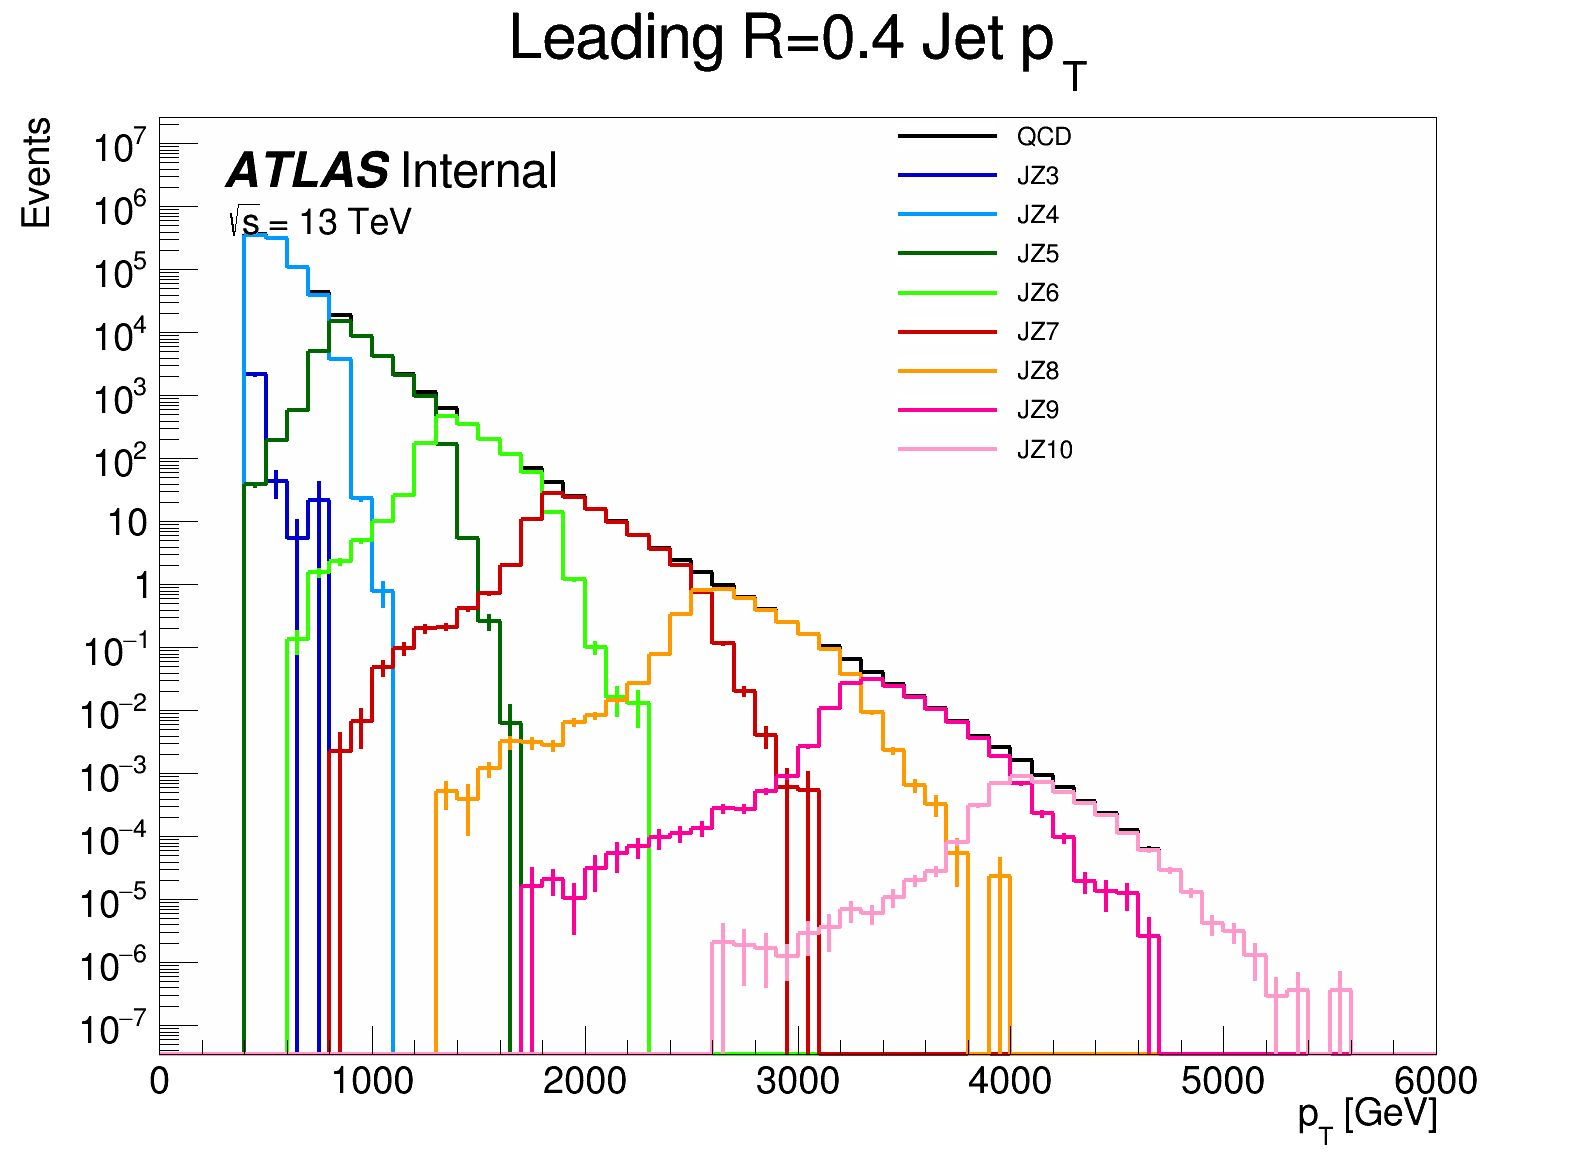
\includegraphics[width=0.49\textwidth]{figures/ch6/jz_slices}
	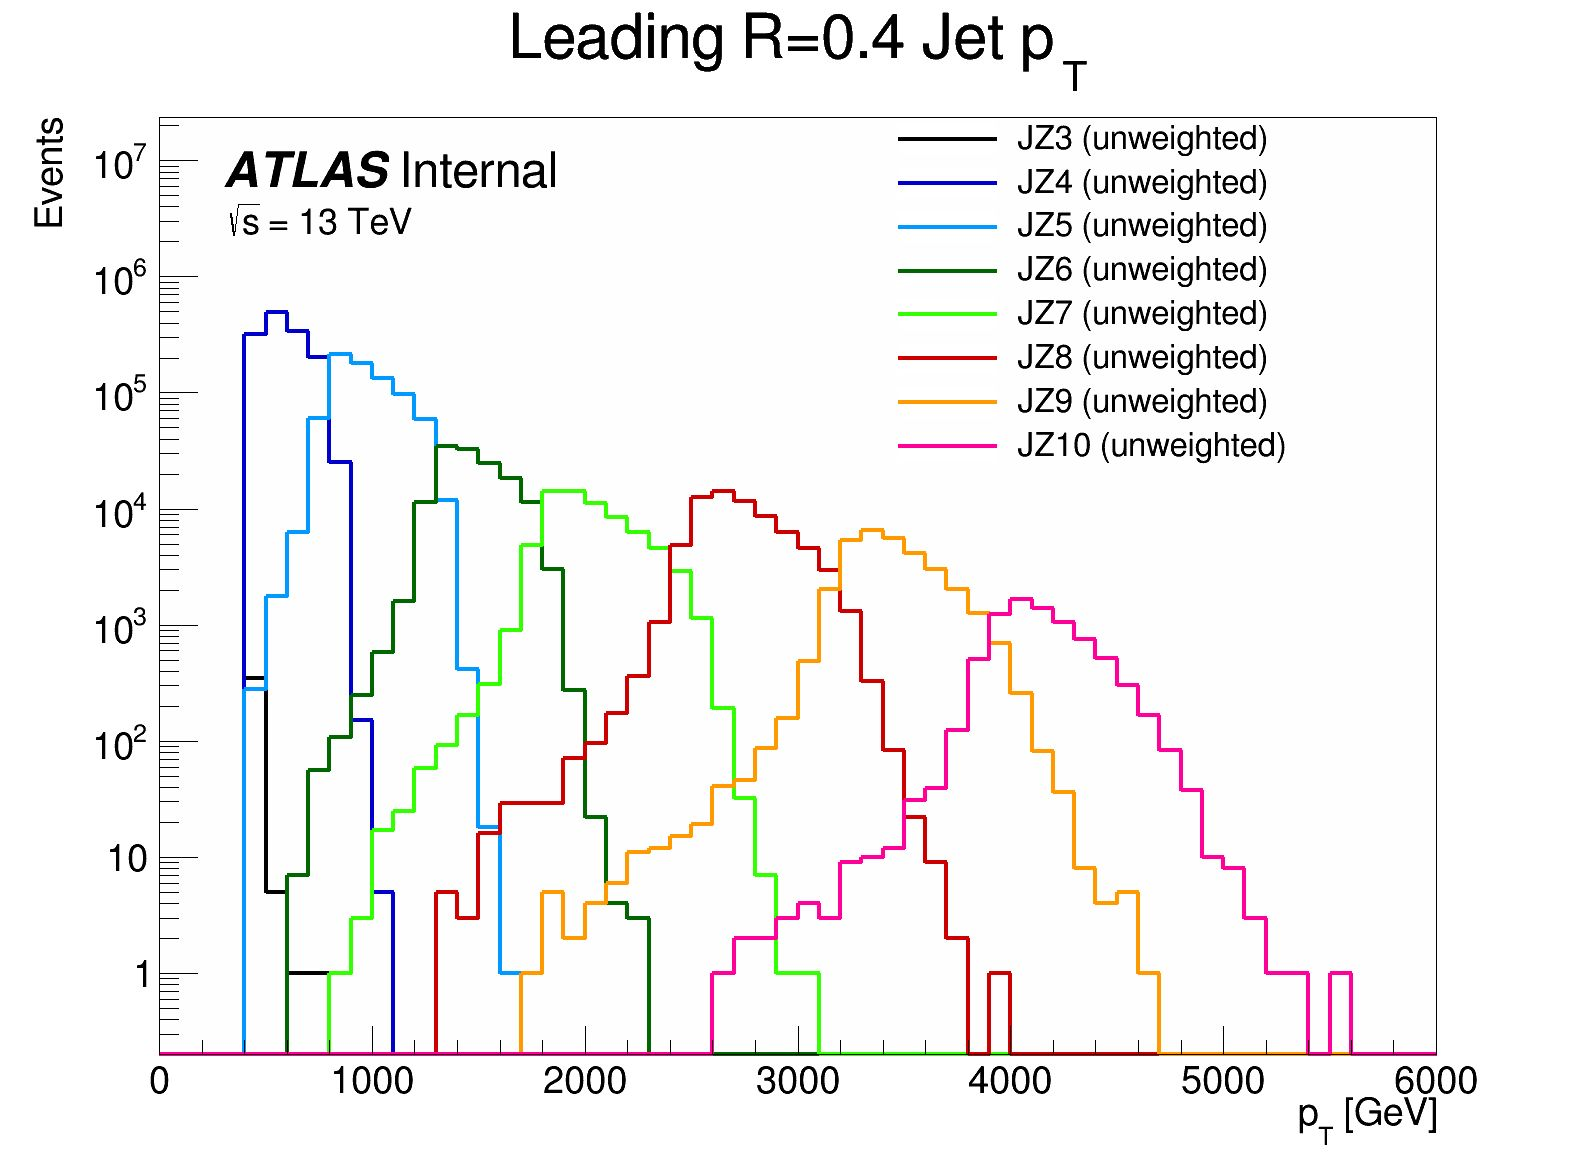
\includegraphics[width=0.49\textwidth]{figures/ch6/jz_slices_uw}
	\caption{The transverse momentum slices of the QCD MC simulation, overlayed to show how they come together to create a smooth distribution (left) once weighted properly. The original unweighted distribution is shown on the right, illustrating the enhanced statistics for the high \pt~range. 
	\label{fig:jzslices}}
\end{figure}

Due to presence of \met in the SVJ signals, additional MC background processes are required to create a full picture of the relevant background. 
The $Z\rightarrow \nu\nu$ process contributes to the background due to its high missing energy. 
Leptonic W/Z decays and W/Z+jets are also included as they can contribute both additional missing energy and significant hadronic activity.
Single top and $t\bar{t}$ processes are also considered for their contribution to hadronic activity.
After the analysis \textit{preselection}\footnote{A preselection is a set of cuts on physical observables used to isolate a collection of events which are most likely to contain the desired signal. The preselection for this analysis will be discussed in Section~\ref{sec:eventsel}} is applied to isolate events most relevant to the SVJ topology, the background composition is 76\% QCD, 12\% $W$+jets, 8\% top and $t\bar{t}$ processes, and 4\% $Z\rightarrow \nu\nu$.  
Figure~\ref{fig:bkg_mc} illustrates the background composition for the analysis.
The lower panel in Figure~\ref{fig:bkg_mc} illustrates the ratio between data (black) and the combined MC processes (grey).
While the agreement between data and MC is not perfect (ratio = 1.0 for all \met~ values), the difference is $<20$\% throughout the distribution.
This is within tolerance for this analysis, since the final background estimation will be data driven, and background MC is only needed for approximate modeling.
Analysis selections for high energy jets (discussed in Section~\ref{sec:eventsel}) create some sculpting in the $Z\rightarrow \nu\nu$ and $W$+jets distributions; however, the total \met~ distribution is smoothly falling so this is not an issue.

\begin{figure}
        \centering
	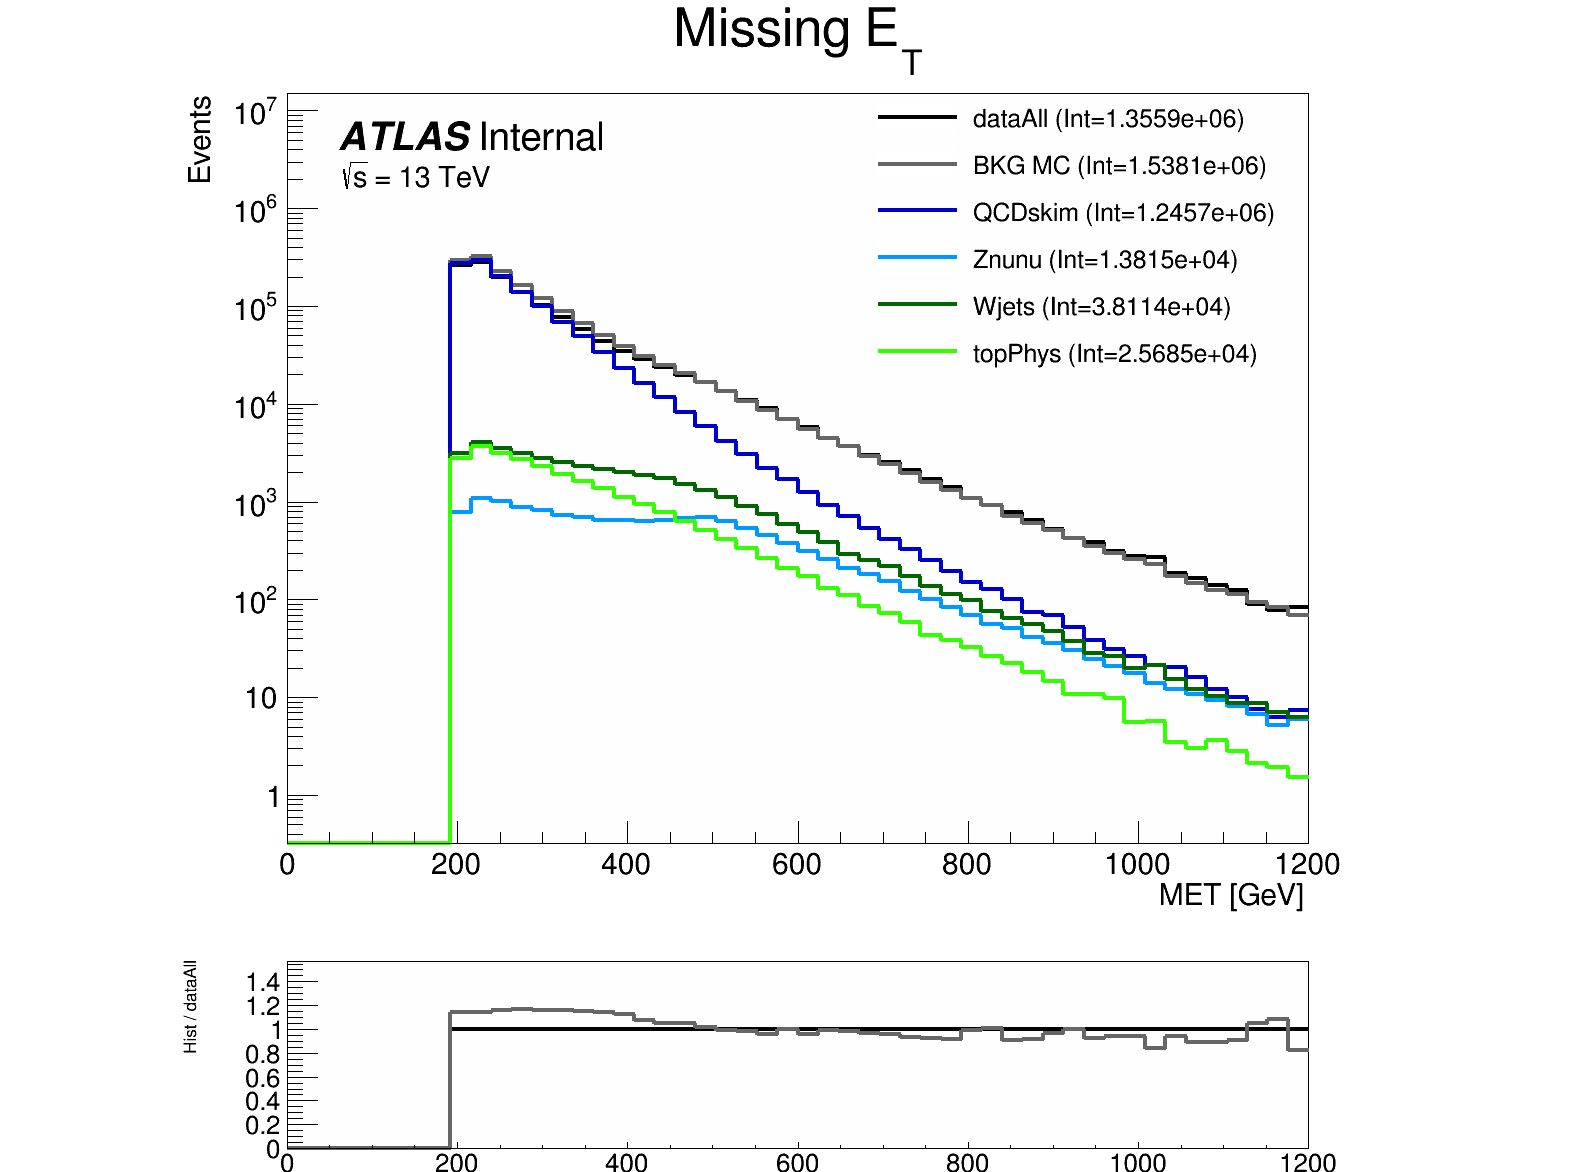
\includegraphics[width=0.55\textwidth]{figures/ch6/bkg_mc}
	\caption{Background processes relevant to the SVJ signal. 
	\label{fig:bkg_mc}}
\end{figure}

\subsection{Signal Simulation}
\label{subsec:signals}

The Hidden Valley (HV) signal model implementation is based on Ref~\cite{darkqcd}. 
The s-channel semi-visible jet model, which was described in Chapter~\ref{ch:theory}, is governed by a number of parameters. 
The mass of the mediator $m_{Z'}$ can be set, together with the couplings of the $Z'$ to the visible and dark quarks $g_q$ and $g_{q_D}$. 
The dark sector shower is governed by the number of dark colors $N_{c_D}$, the number of dark flavors $N_{f_D}$, and the dark sector confinement scale $\Lambda_D$. 
There is also the characteristic scale of the dark hadrons $m_{dark}$, determined by the mass of the dark quarks $m_{q_D}$. 
The characteristic scale determines the mass of the dark hadrons, which can be pseudoscalars $m_{\pi_D}$ or vectors $m_{\rho_D}$.
Finally, the average fraction of invisible particles in the final state jet is dictated by \rinv. 

%Our choices of these parameters are informed by the 2021 Snowmass report~\cite{snowmass}. 
The chosen parameters for this model were carefully selected in collaboration with theorists to be compatible with the new benchmarks established in the 2021 Snowmass process~\cite{snowmass}. 
The signal generation allows for up to two initial state radiation jets, and uses a jet-matching scheme described in Ref.~\cite{mlm} and implemented in Ref.~\cite{pythia} to match jets to the original partons.
%A notable remaining difference between the ATLAS s-channel and t-channel searches 

The choices of fixed parameters for the Pythia8 HV model are summarized in Table \ref{tab:model_fixed_params}.
A detailed discussion of these parameters and their implications on the dark shower topology can be found in Ref.~\cite{snowmass}. 
The mass choices for the dark quark and the dark hadrons are also summarized in Table \ref{tab:model_mdark}. 

\begin{table}
\centering
  \begin{tabular}{ |c|c| }
    \hline
    Parameter & Value \\
    \hline
     $N_{c_D}$ & 3.0 \\
     $\Lambda_D$ & 10.0 GeV\\
     $N_{f_D}$ & 2.0\\
     $g_q$ & 0.25\\
     $g_{q_D}$ & 0.5\\
    \hline
  \end{tabular}
  \caption{Fixed parameters in the Pythia8 HV model}
  \label{tab:model_fixed_params}
\end{table}

Note that the number of dark flavors differs from the Snowmass recommendation of $N_{f_D}$ = 4. 
This change is minimal in impact because \rinv~is set explicitly (rather than allowing it to arise naturally from the HV theory), and allows this ATLAS analysis result to remain comparable with the CMS semi-visible jets s-channel analysis \cite{cms_svj} and the ATLAS semi-visible jets t-channel analysis \cite{tchannel}. \par

\begin{table}
\centering
  \begin{tabular}{ |c|c| }
    \hline
    Parameter & Value [GeV] \\
    \hline
     $m_{\pi_D}$ & 17.0 \\
     $m_{\rho_D}$ & 31.77 \\ 
     $m_{q_D}$ & 10.0 \\ 
    \hline
  \end{tabular}
  \caption{Values for $m_{dark}$}
  \label{tab:model_mdark}
\end{table}

The mediator mass $m_{Z'}$ and the fraction of invisible particles in the final state \rinv~vary, and are used to define the search grid. $m_{Z'}$ varies between 2.0 TeV and 5.0 TeV, while~\rinv~ varies from 0.2 to 0.8. \rinv~values of 0.2, 0.4, 0.6, and 0.8 are generated for each $m_{Z'}$ mass point. Table \ref{tab:sig_grid} illustrates the signal grid and the associated cross-section for each signal. There are a total of 24 signal points (6 $Z'$ masses $\times$ 4 \rinv~settings) considered in this analysis.

\begin{table}
\centering
  \begin{tabular}{ |c|c| }
    \hline
    $m_{Z'}$ (GeV) & Cross section (fb)  \\
    \hline
     2000 &  252 \\
     2500 &  74.2 \\
     3000 &  24.5\\ 
     3500 &  8.83\\
     4000 &  3.49 \\ 
     5000 &  0.757 \\
    \hline
  \end{tabular}
  \caption{Mass points and cross sections of the SVJ search signal grid. The cross section is determined only by the $Z'$ mass and is not impacted by the \rinv. }
  \label{tab:sig_grid}
\end{table}

Samples are generated using 
\textsc{MadGraph5}~\cite{Alwall:2014hca} version 2.9.9 interfaced to 
\textsc{Pythia8.244p3}~\cite{pythia} for shower and hadronization with 
NNPDF23LO PDF~\cite{Butterworth:2015oua} and the 
ATLAS A14~\cite{Skands:2014pea} to tune the underlying event data.


%%%%%%%%%%%%%%%%
% Chapter 7
%%%%%%%%%%%%%%%%
\chapter{Machine Learning Tools}
\label{ch:ml_tools}

\section{Introduction}
The search for semi-visible jets presents an opportunity to use novel machine learning (ML) tools to uncover patterns in the behavior of dark QCD. The subtlety of the shower differences between dark and SM QCD motivates a complex model that can accept high-dimensional low-level inputs to best understand key differences between signal and background correlations. Additionally, the large number of theory parameters which can be chosen arbitrarily and affect the shape of the dark QCD shower motivate exploring a data-driven machine learning approach, which could be sensitive to a wider variety of dark QCD behavior. \par

To this end, two machine learning approaches are developed for this search, which are used in tandem. The first is a supervised ML method where the ML algorithm is built to maximize exclusion sensitivity to the specific generated SVJ signal models used in this analysis. Here, supervised refers to the use of full and correct labels for all events considered during model training, which necessitates training over simulated data. The second is a semi-supervised method, where training of the model is data-driven and labels are only partially provided during training. The semi-supervised ML algorithm broadens the discovery sensitivity of the search, and reduces the dependence on the exact theory parameters chosen for signal model simulation. \par

The two different ML algorithms used in this approach will be explained in the following sections, along with their application in the SVJ analysis strategy.

%------------------------------------------------
\section{Particle Flow Network (Supervised)}
\label{subsec:supervised}
The supervised machine learning approach maximizes discovery sensitivity for the SVJ signals considered in this thesis.
The networks learns the features of the SVJ signals, allowing the network to be highly efficient in selecting events that resemble the SVJ signal.

\subsection{Architecture Fundamentals}

A Particle Flow Network (PFN)~\cite{pfn} architecture is selected for two reasons: \textit{permutation invariant input modeling} to best describe the events consisting of an unordered set of particles, and a \textit{low-level input modeling} to take advantage of the ability of neural networks to uncover patterns in high-dimensional data. \textit{Low-level} refers to using detector level information such as individual particle tracks, rather than \textit{high-level} information such as reconstructed jet objects. Low-level inputs are generally high-dimensional; for instance, an event may have only 2 jets (dim-2), but each jet consists of 70 particles (dim-140). Low-level input modeling is chosen to capture the intricacies of dark QCD showers with may not express themselves in high level objects, as explored in Ref.~\cite{darkqcd}. Permutation invariant input modeling is chosen as the most accurate representation of a set of particles. In previous work such as Ref.~\cite{vrnn}, ordered input modeling has been observed to \textit{bias} the performance of low-level modeling tools. In this case bias means that the performance of the tool was observed to change substantially depending on the input ordering; however, there is no physics motivation for choosing any particular order. 

The input to the PFN is a collection of particles and their associated physics information, such as momentum and trajectory. Constructing the PFN involves the creation of new basis variables $\Phi$ for each particle in the input event. This transformation is summarized as $\vec{p_i} \rightarrow \vec{\Phi_i}$ where $\vec{p_i}$ is the physics information for the $i$th particle in the event, and $\vec{\Phi_i}$ is that same information encoded into the $\Phi$ basis. Permutation invariance is enforced by summing over the $\Phi$ basis for every particle in the event to create a new permutation invariant event representation $\mathcal{O}$. The creation of $\mathcal{O}$ from $M$ particles $\vec{p}$ with $d$ physics features each can be expressed as:

\begin{equation}
  \mathcal{O}(\{\vec{p_1},...,\vec{p_M}\}) = \sum_{i=1}^M \Phi_i(\vec{p_i})
  \label{eq:pfn}
\end{equation}

where $\Phi : \mathbb{R}^d \rightarrow \mathbb{R}^l$ is a per particle mapping, with $l$ being the dimension of the new basis $\mathcal{O}$. Figure~\ref{fig:pfn_paper} gives a graphical representation of the use of summation in the PFN over per-particle information to create a permutation-invariant event representation. \par
\begin{figure}[!htbp]
\centering
   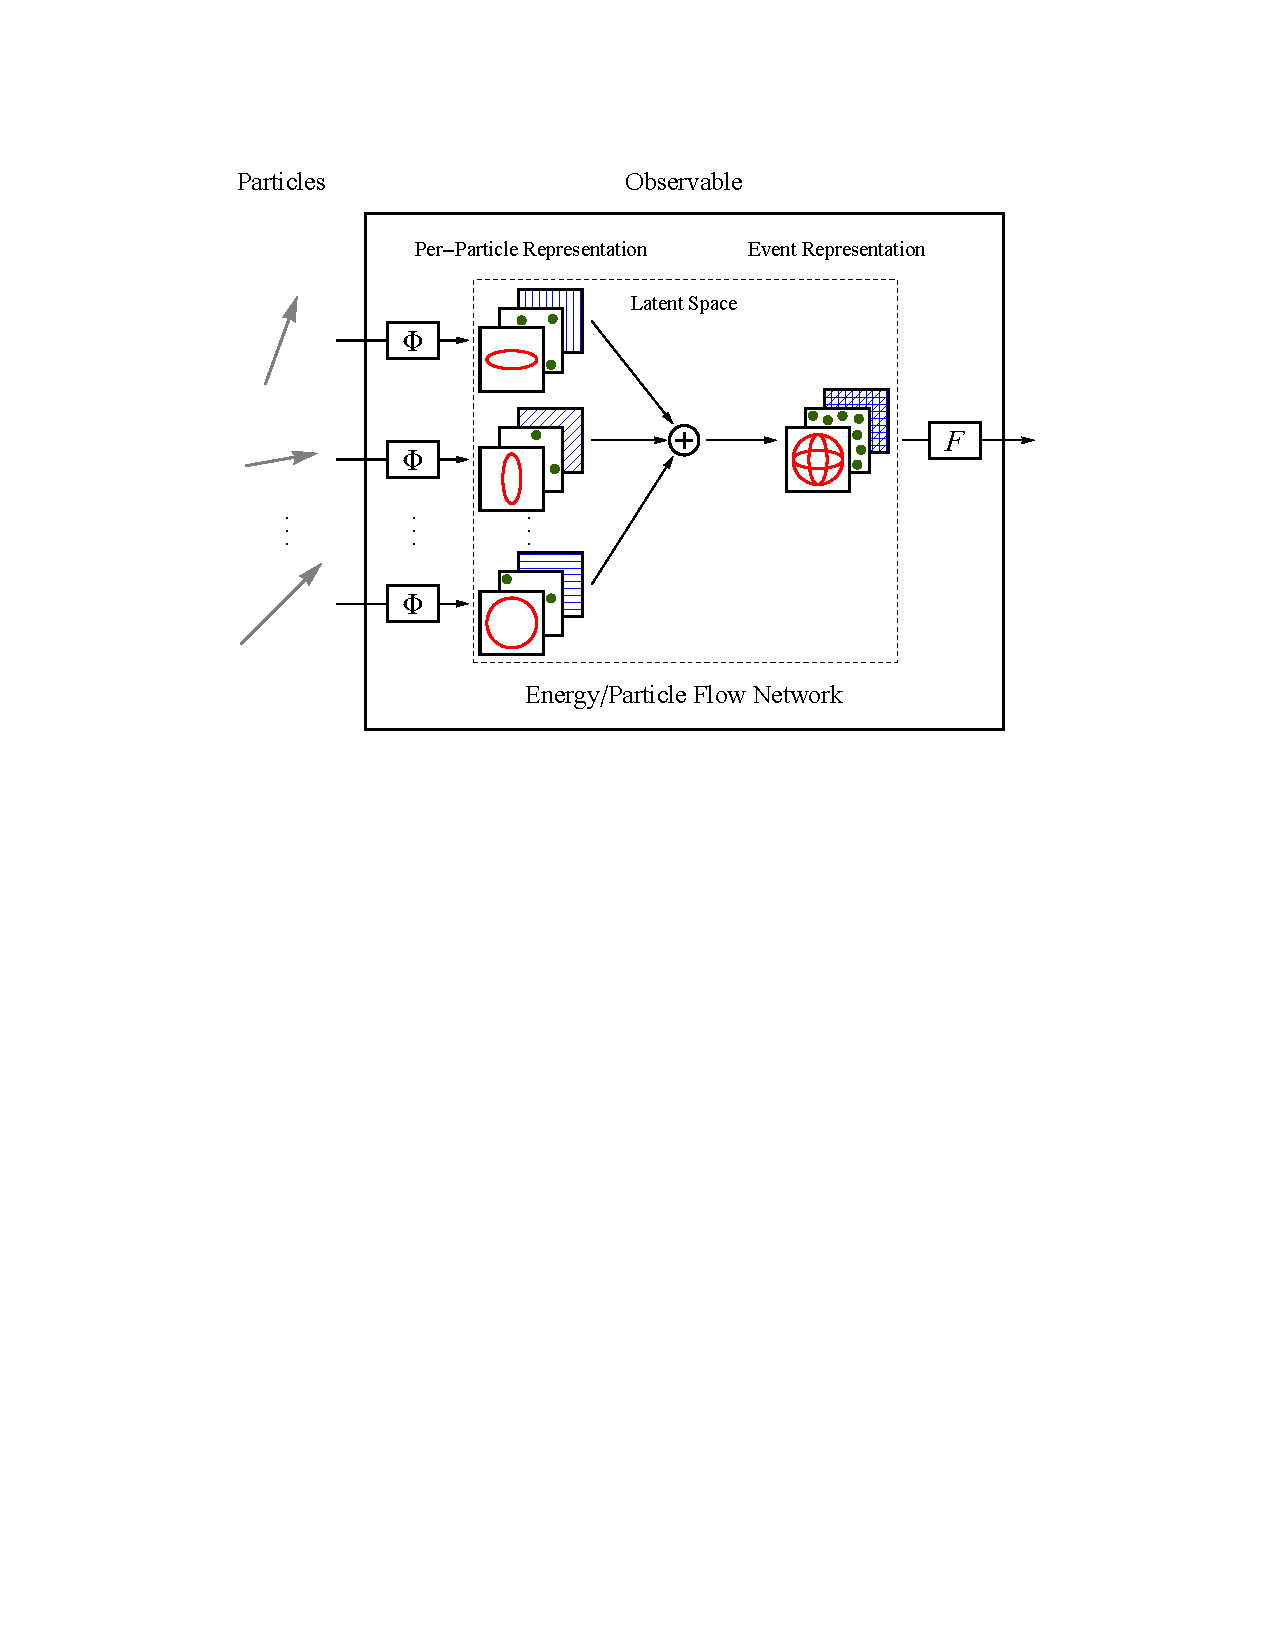
\includegraphics[width=0.7\textwidth]{figures/ml/pfn_paper}
    \caption{The Energy/Particle Flow Network concept, from Ref.~\cite{pfn}. The physics input information is represented as arrows on the left, for an arbitrary number of particles. The $\Phi$ transformation converts these arrows to 3 graphs, indicating the $\Phi$ basis dimension $l$ is 3 in this example. The graphs are then summed for all particles to create $\mathcal{O}$, or the event representation.
    \label{fig:pfn_paper}}
\end{figure}

The $\Phi$ basis transformation is implemented via a deep neural network. The output of the neural network is summed as indicated in Equation~\ref{eq:pfn} to create the new permutation invariant event representation $\mathcal{O}$. $\mathcal{O}$ then becomes the input of a second deep neural network $F$. $F$ is a classifier network which separates signal and background events. Figure~\ref{fig:pfn_arch} provides an annotated diagram of the PFN architecture as used in this analysis. 
\begin{figure}[!htbp]
\centering
   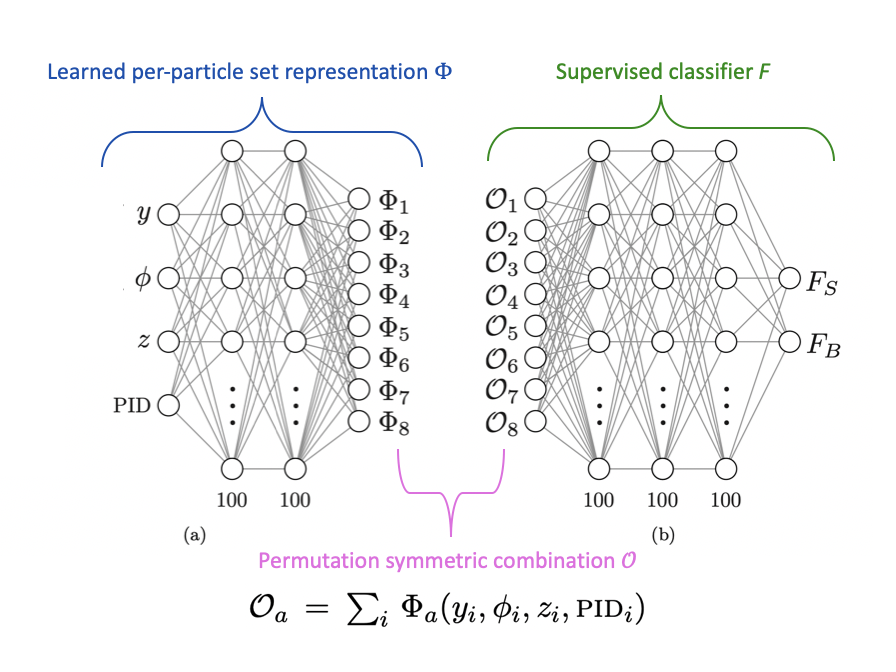
\includegraphics[width=0.8\textwidth]{figures/ml/pfn_arch}
    \caption{An annotated diagram of the PFN architecture~\cite{pfn}. $y$ and $\phi$ represent geometric trajectory information for the input particles, $z$ represents energy information, and PID encompasses any other particle ID information in the input. PID is presented in the diagram as a 1-dimensional input, but could represent multiple input dimensions.
        \label{fig:pfn_arch}}
\end{figure}

%--------------------
\subsection{Input Modeling, Scaling, and Rotation}
\label{sec:input_model}
In this implementation, the particle input information comes from all tracks associated to the leading and subleading jets. The track association method is Ghost association, as discussed in Section~\ref{sec:ghost}. A single jet tagger strategy was also considered, but utilizing tracks from both leading jets creates a more complete low-level picture of the event. The choice of the two leading jets is justified in Chapter~\ref{ch:analysis}. If we consider the dijet topology of semi-visible jets as illustrated in Figure~\ref{fig:svj_pic}, the advantage of modeling both leading jets simultaneously becomes clear. In the semi-visible jet model presented in Ref.~\cite{darkqcd}, \met~in the event is expected to arise due to an imbalance in the number of visible tracks of the two jets associated to the dark quark decay.\par

\begin{figure}[!htbp]
\centering
   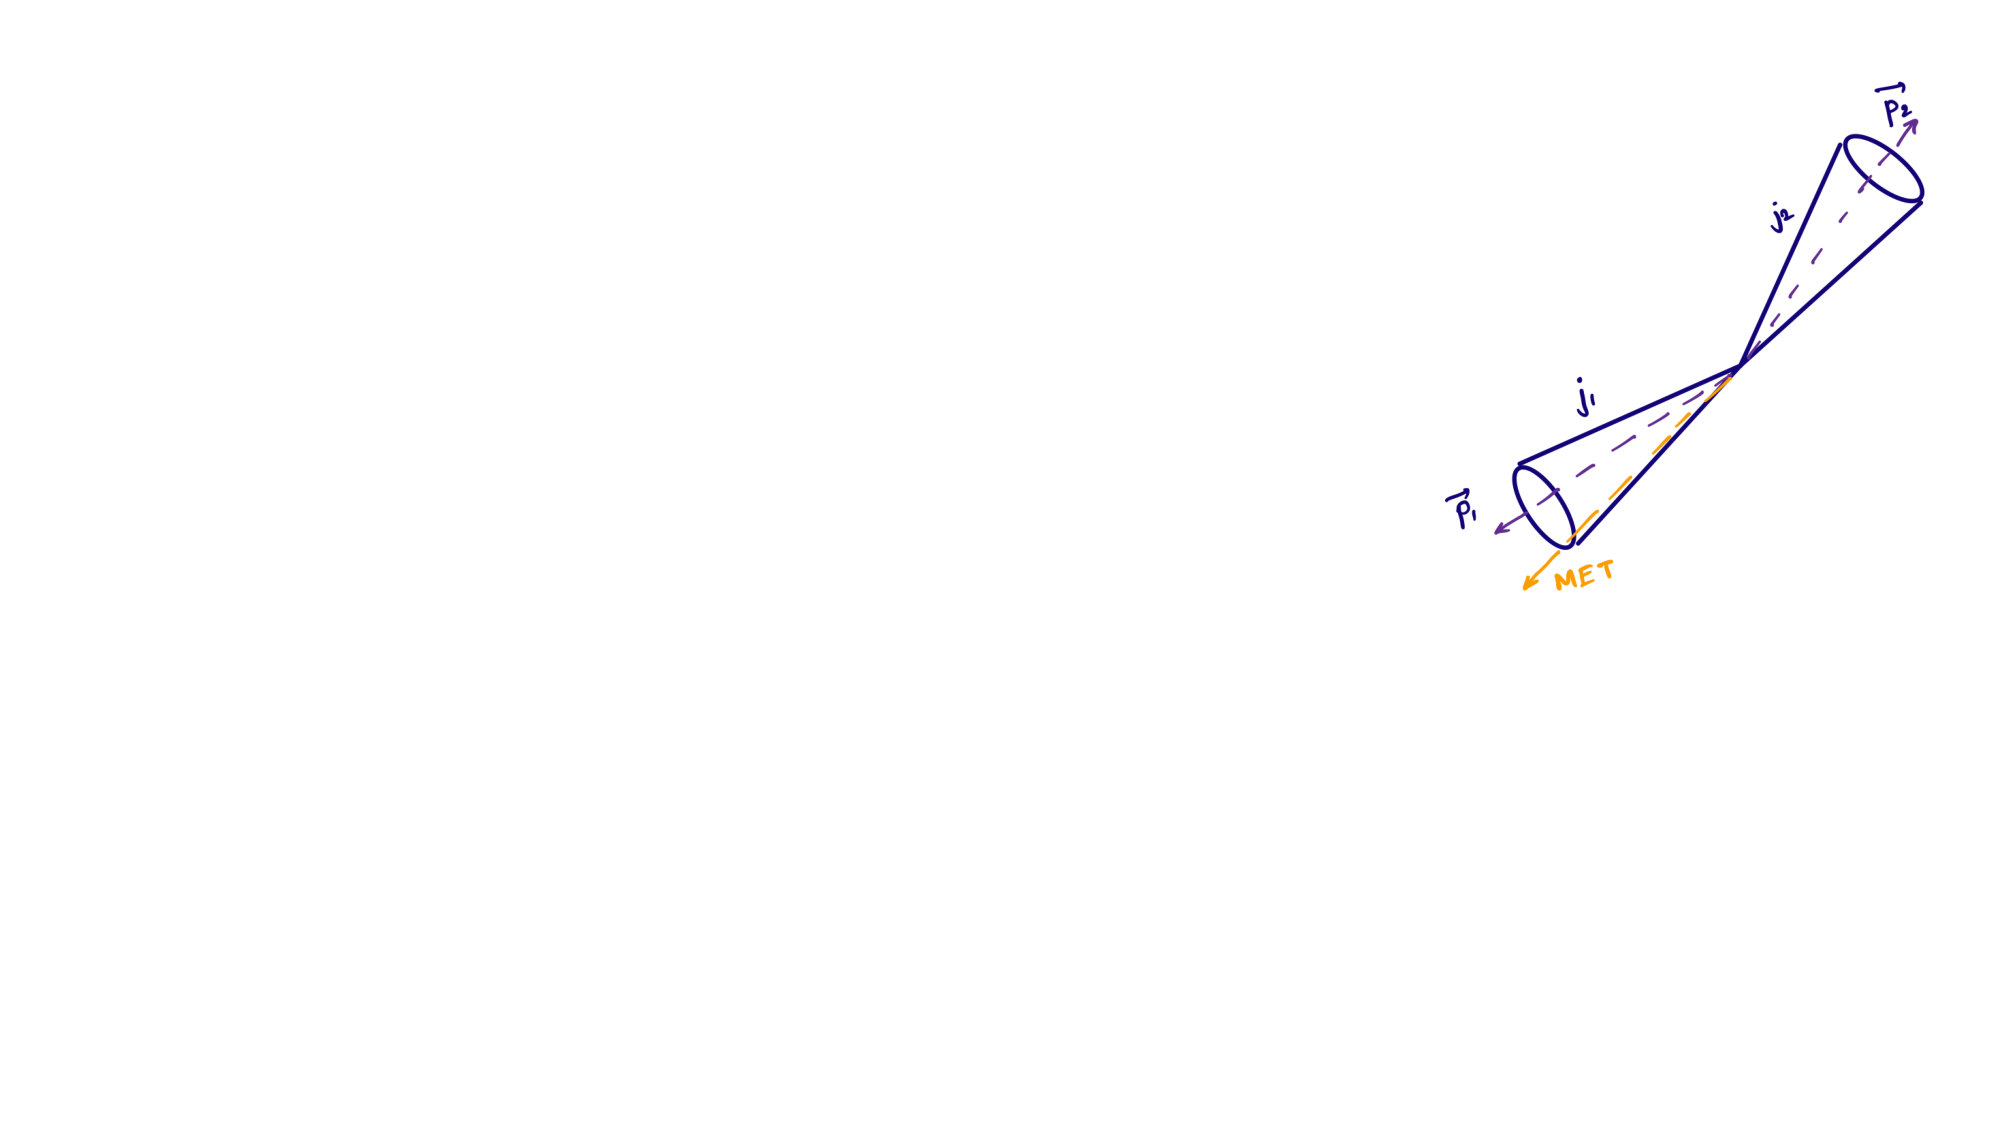
\includegraphics[width=0.4\textwidth]{figures/ml/dijet_topology}
    \caption{An illustration of the expected dijet behavior of semi-visible jets, where one jet is closely aligned with \met (MET). In the figure two jet cones $j_1$ and $j_2$ are illustrated, along with their associated momentum vectors $\vec{p_1}$ and $\vec{p_2}$. 
        \label{fig:svj_pic}}
\end{figure}

Each track is described using six variables: the four-vector of the track (\pt, $\eta$, $\phi$, E), and the track displacement parameters $d_0$ and $z_0$, where $d_0$ measures displacement in the radial direction from the beamline and $z_0$ measures displacement along the beamline from the primary interaction point. Figure~\ref{fig:trackcoordinates} illustrates these coordinates. Up to 80 tracks per jet are allowed, which is a threshold chosen to generally include all the tracks in the jet, which leads to maximal performance.\par %Figure~\ref{fig:ntracks} shows the track multiplicity in the leading and subleading jet for the signal and background samples used in training. \par

\begin{figure}[!htbp]
\centering
   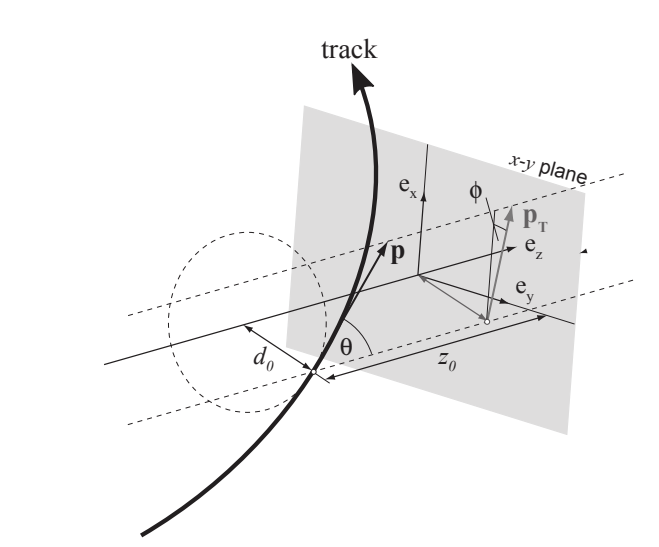
\includegraphics[width=0.4\textwidth]{figures/ml/trackcoordinates}
    \caption{Illustration of track coordinates $d_0$ and $z_0$.
    \label{fig:trackcoordinates}}
\end{figure}

%\begin{figure}[!htbp]
%\centering
 %  \includegraphics[width=0.95\textwidth]{figures/ml/ntracks}
 %   \caption{Distributions of the track multiplicity in the leading and subleading jets, comparing signal and background PFN training samples.
%    \label{fig:ntracks}}
%\end{figure}

These tracks (up to 160 total) are the input to the PFN. Referencing Equation~\ref{eq:pfn}, this corresponds to $M = 160$ (number of particles) and $d = 6$ (number of features per particle). The two leading jets and their associated tracks are rotated so that the vector sum of the jets, or system average, is aligned with $(\eta,\phi) = (0,0)$. The rotation can be summarized as 
\begin{subequations}
    \begin{align}
       \eta_{i}' &= \eta_i - \bar{\eta},  \\
        \phi_{i}' &= \phi_i - \bar{\phi}
    \end{align}
\end{subequations}
where ($\bar{\eta}, \bar{\phi}$) is the average angle of the dijet system,  ($\eta_{i}, \phi_{i}$) are the original track coordinates, and ($\eta_{i}', \phi_{i}'$) are the rotated track coordinates. Figure~\ref{fig:jet_rotate} illustrates the rotation process. The rotation ensures that the information used by the algorithm is the relative orientation of the jets (and associated tracks) to each other, not their absolute position in the detector. Each track is normalized to its relative fraction of the total dijet system energy and transverse momentum; this enforces agnosticism to the total energy and transverse momentum of the event. The rotation and scaling are motivated by the procedures described in Ref.~\cite{pfn} to improve the performance of the PFN. 

\begin{figure}[!htbp]
\centering
   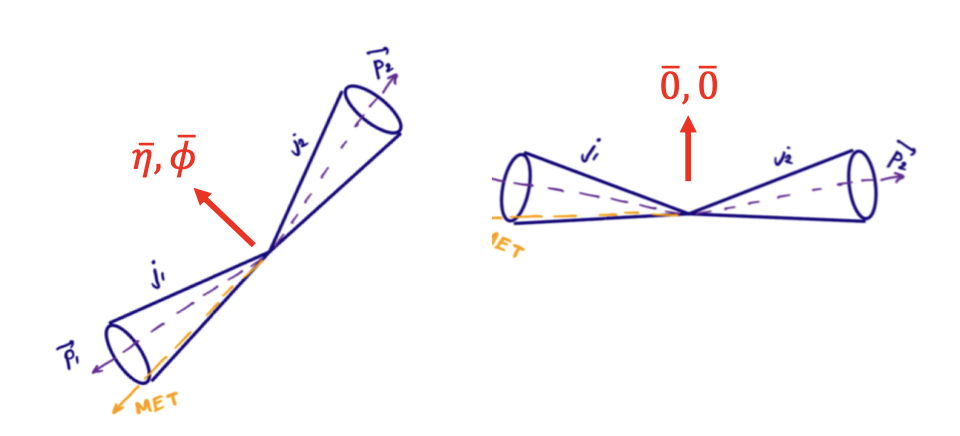
\includegraphics[width=0.65\textwidth]{figures/ml/jet_rotate}
    \caption{A diagram demonstrating how the two jet system is rotated in $(\eta,\phi)$. The jet cones and associated jet tracks are illustrated. The dashed tracks represent dark hadrons while the solid tracks represent SM hadrons. The system average $(\bar{\eta},\bar{\phi})$ is shown in red and an example track with coordinates $(\eta_i,\phi_i)$ is shown in purple.
    \label{fig:jet_rotate}}
\end{figure}

Finally, each of the 6 track variables is scaled so that its range is [0,1]. This is a common preprocessing step that ensures the input data is bounded over a similar range, so that arbitrarily large values don't develop an outsized impact on the model. The track momentum and energy normalization mentioned above naturally enforces that these values are restrained between [0,1]. The $\eta$ and $\phi$ values are naturally bounded, so for these values the $\eta$ tracking range\footnote{This range is dictated by the $|\eta|$coverage range of the Inner Detector, as shown in Table~\ref{tab:atlas_requirements}} of [-2.5, 2,5] and the full $\phi$ range [$-\pi$, $\pi$] are mapped to [0,1]. The displacement variables are restricted to [0,1] via the standard \textsc{MinMaxScaler}~\cite{scikit-learn} method which determines the minimum and maximum values observed in training, and maps those boundaries to 0 and 1 respectively. \par

Figure~\ref{fig:pfn_datamc_input} illustrates that the data is well modeled by the MC at track level. Figure~\ref{fig:pfn_bkgsig_input_kin} shows the kinematics of each of 6 track variables for background and signal. Figure~\ref{fig:pfn_bkgsig_input_rot} shows each of the 6 track variables after scaling and rotation have been applied, demonstrating the impact of these procedures, as well as the track level similarities and differences between the background SM QCD processes and the signal SVJ processes. \par

The $\phi$ distribution is of note for its jagged appearance in QCD MC. This arises due to dead tile calorimeter cells in certain $\phi$ regions, the effects of which are seen in data and modeled in QCD MC but not modeled in SVJ signal MC. Appendix~\ref{subsec:tileCal} contains more information about how the issue was addressed in data. The distribution is not of concern for the PFN training because of the rotation process, which replaces the information about absolute detector $\phi$ measurements with the relative $\phi'$ measurement. This is illustrated in Figure~\ref{fig:pfn_bkgsig_input_rot}, where it is observed that for both signal and background the tracks are clustered back to back, centered at $-\pi$/2 and $\pi$/2 (0.25 and 0.75 after scaling). The only remaining difference is that the signal tracks are more likely to be close to the system average $\bar{\phi}$ than the background jet tracks. This is demonstrated by the excess of signal events in the center of the $\phi'$ plot. This orientation difference is a real feature of the signal model, confirmed in Figure~\ref{fig:presel_vars2} which illustrates that signal jets are more likely to have low $\Delta\phi$ than background jets. 

\begin{figure}[!htbp]
   \centering
   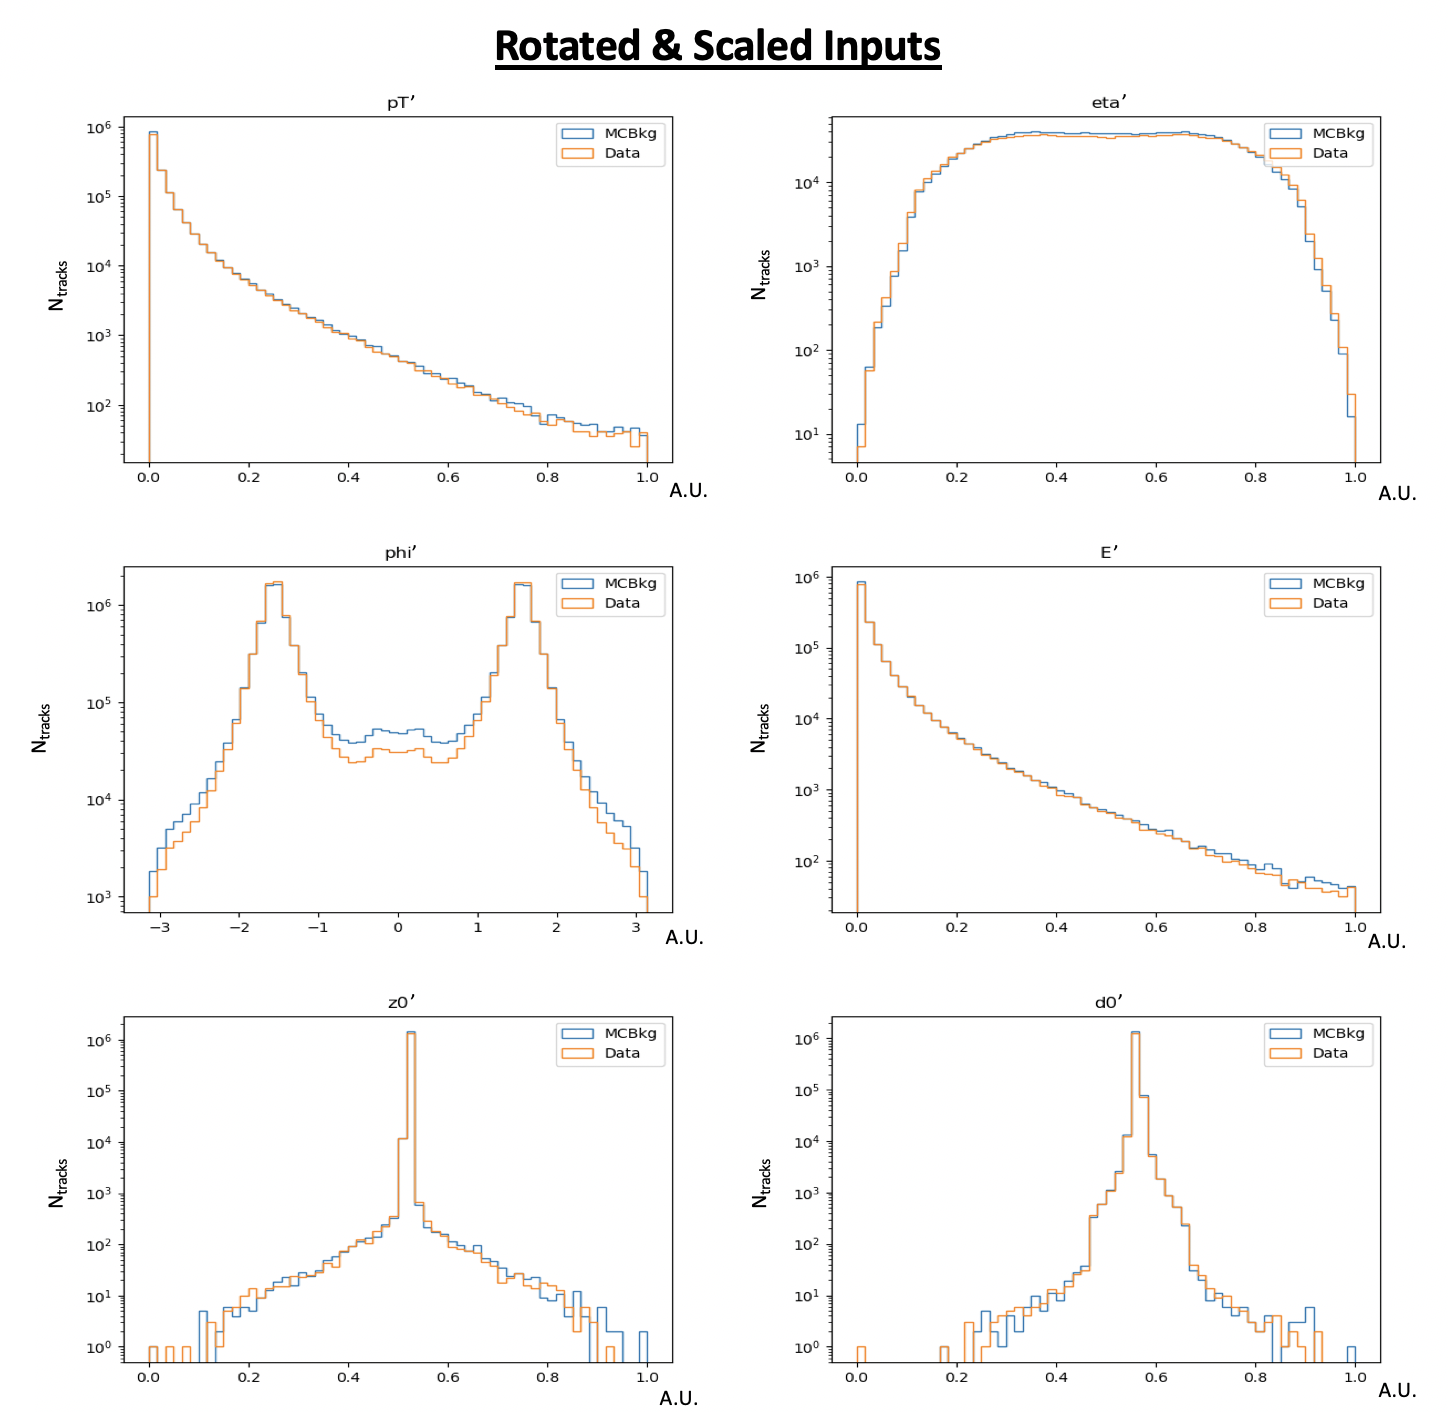
\includegraphics[width=0.99\textwidth]{figures/ml/pfn_datamc_input}
    \caption{The 6 PFN track variables in background MC (blue) and data (orange), after the scaling and rotation procedure is applied. There is excellent modeling of the data by the MC within the track variables. The slight discrepancy in the $\phi$ distribution due to the inaccuracies of modeling dead TileCal cells in the QCD MC is considered. The level of discrepancy is determined to be within tolerance given that the final result with be data driven and the QCD model is used in the PFN training only.
    \label{fig:pfn_datamc_input}}
\end{figure}

\begin{figure}[!htbp]
    \centering
     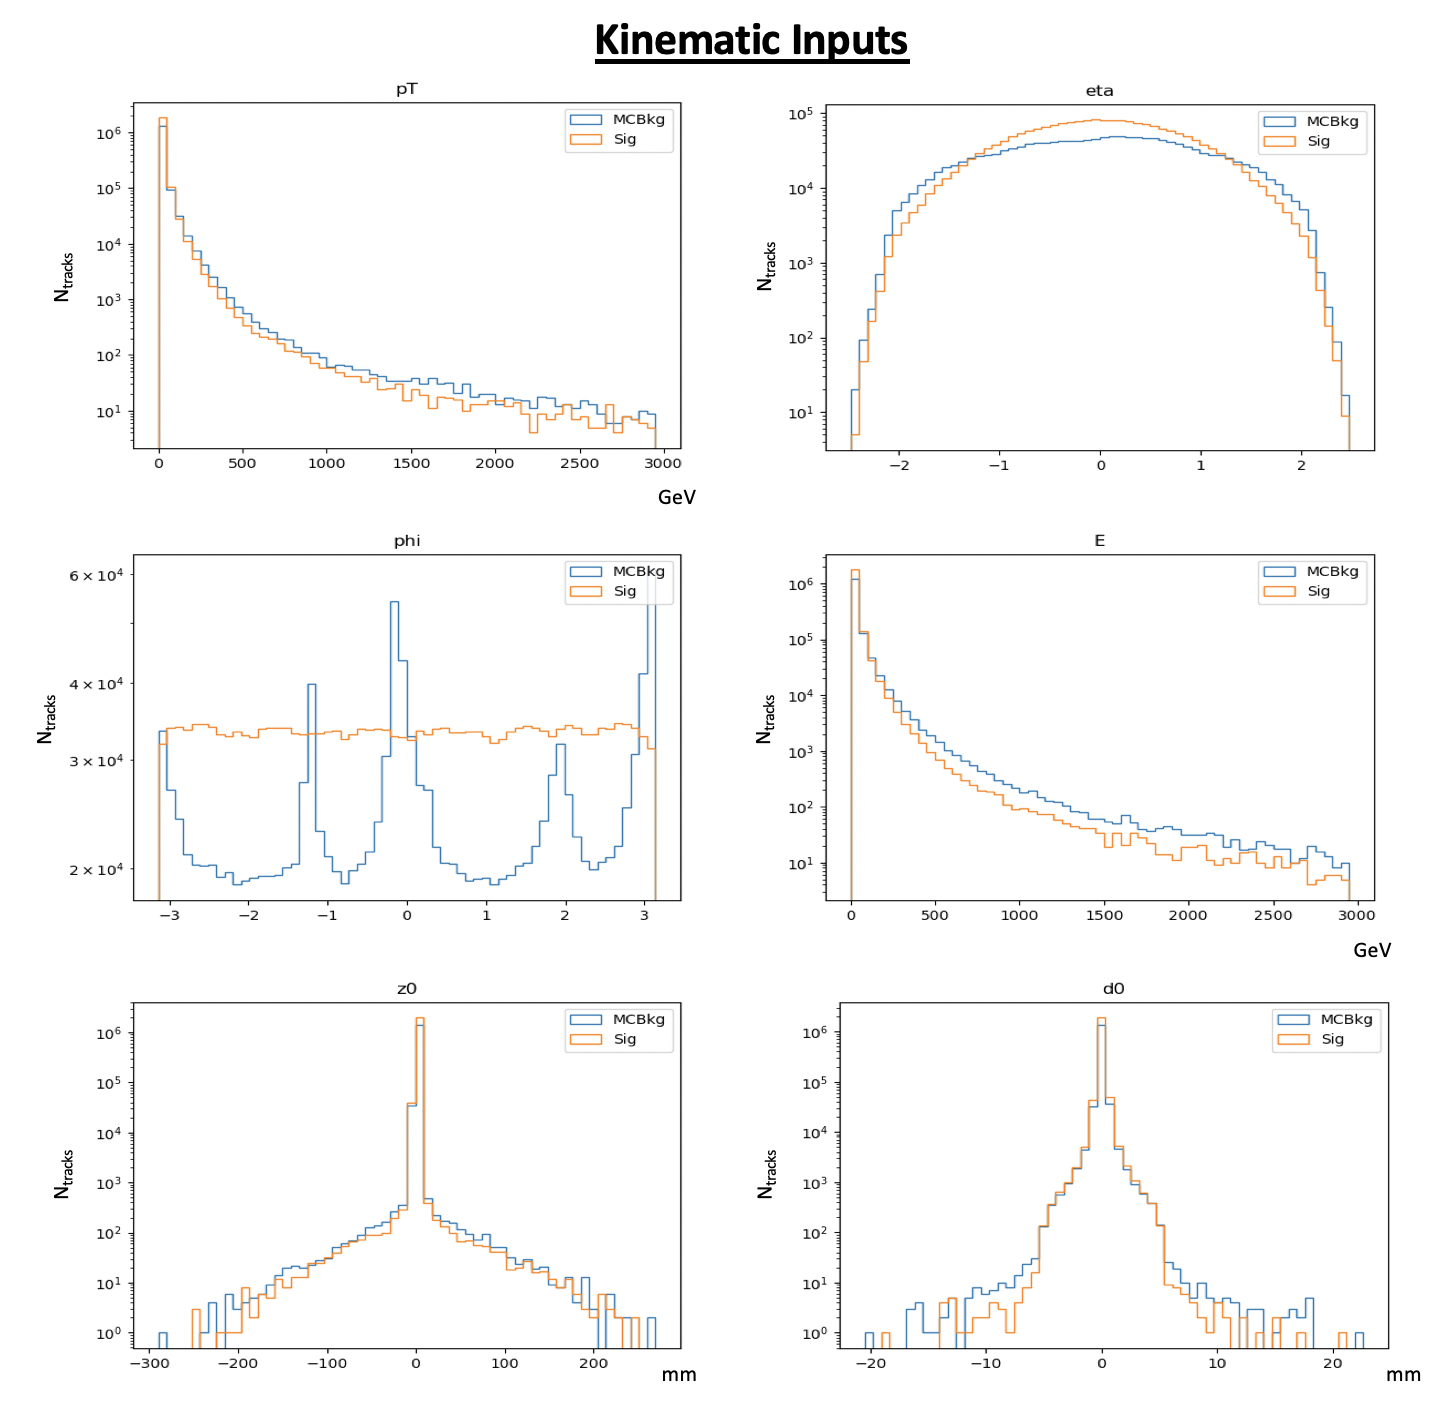
\includegraphics[width=0.99\textwidth]{figures/ml/pfn_bkgsig_input_kin}
     \caption{The 6 PFN track variables in background MC (blue) and signal MC (orange) before scaling and rotation. The track kinematics are largely similar, and the variation in the $\phi$ distribution is explained in the text.}
      \label{fig:pfn_bkgsig_input_kin}
\end{figure}

\begin{figure}[!htbp]
    \centering
    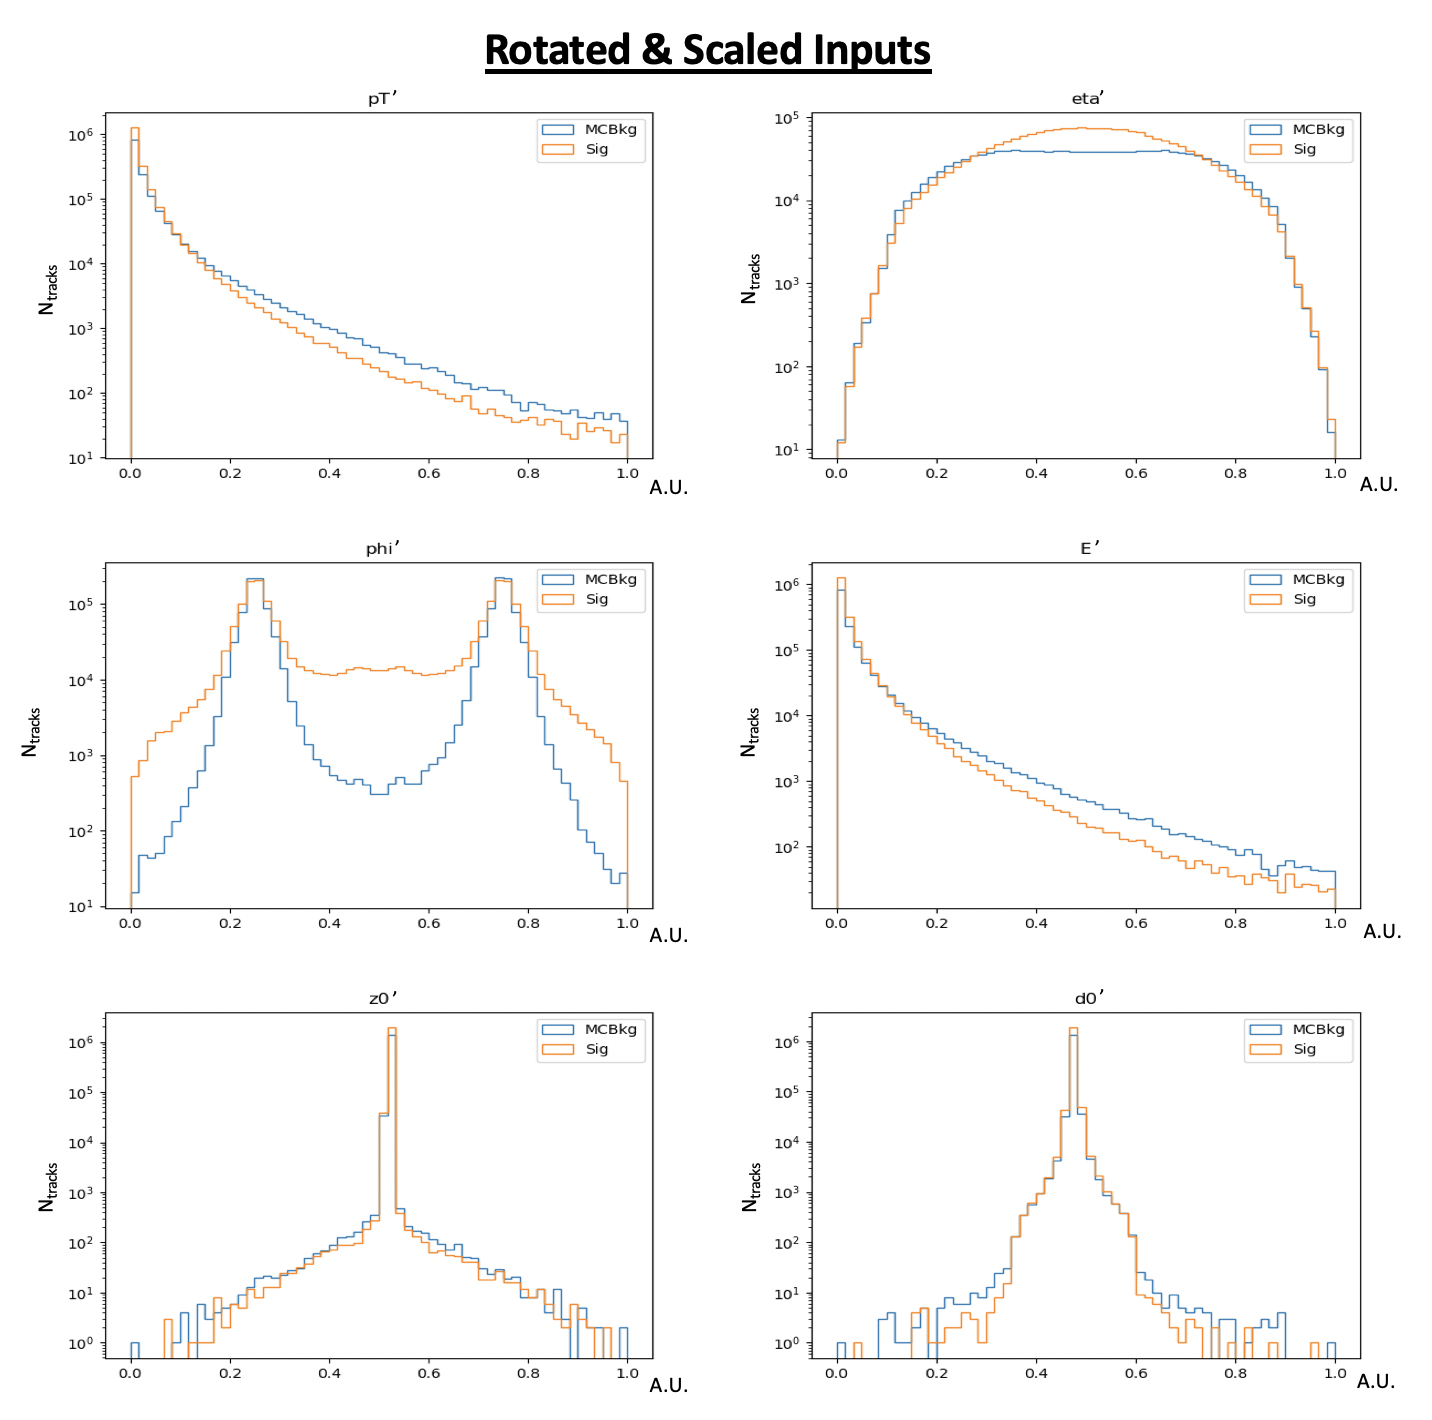
\includegraphics[width=0.99\textwidth]{figures/ml/pfn_bkgsig_input_rot}
     \caption{The 6 PFN track variables in background MC (blue) and signal MC (orange) after scaling and rotation. The $\phi$ distribution is modified by the rotation procedure, as explained in the text.}
     \label{fig:pfn_bkgsig_input_rot}
\end{figure}

\clearpage

%--------------------
\subsection{Training}
\label{sec:pfn_training}

As seen in Figure~\ref{fig:pfn_arch}, two networks are defined and combined for the PFN architecture. In our implementation the input layer has a dimension of 6, accounting for the 6 track variables described in the previous section. The first network, termed the $\Phi$ network, creates the per-particle set representation as illustrated in Figure~\ref{fig:pfn_paper}. The $\Phi$ network has 2 hidden layers each of dimension 75, and an output later of dimension 64. These dimensions were chosen via an optimization procedure which balanced network complexity (achieved with more dimensions) against training time (achieved with fewer dimensions). The two hidden layers and $\Phi$ output layer all use a \textsc{relu} activation function~\cite{scikit-learn}, following the work of Ref.~\cite{pfn}. 

The input layer of the classifier $F$ network is required to have the same dimension as the output layer of the $\Phi$ network, and therefore takes dimension 64. This network contains 3 hidden layers with 75 nodes each, and again uses \textsc{relu} activation~\cite{scikit-learn}. The final layer is the binary classifier result with dimension 2, which uses a \textsc{softmax} activation~\cite{scikit-learn} that is well suited for classification. The loss function for the complete PFN network is \textsc{CategoricalCrossentropy}~\cite{scikit-learn}, which is a standard loss function for DNN classifiers. The standard Adam optimizer~\cite{adam}~\cite{scikit-learn} is used with a learning rate of 0.001. The learning rate was reduced from the nominal learning rate of 0.01 presented in Ref.~\cite{pfn} to prevent overtraining.\par

The PFN is a supervised algorithm, and is therefore trained on a labeled mixture of signal and background events. The signal input is an even mixture of all signal points considered in this analysis. Although the full simulated background for this analysis is composed of several SM processes as discussed in Section~\ref{subsec:bkg_mc}, QCD is the dominant background. Training with a QCD-only background sample is determined to produce better results than training using the full background mixture. Including MC backgrounds that are enriched in \met~(recall Figure~\ref{fig:bkg_mc}) reduces the ability of the PFN to classify SVJ signals. This is illustrated in the comparison of output classifier distributions in Figure~\ref{fig:pfn_MC_training_mixture}. The signals used for training are the same in both cases. When training with a QCD-only background, high \met~data and MC is more likely to be classified as signal like; however the increased signal performance means that overall \textit{sensitivity}\footnote{Sensitivity is a measure of the ability of an analysis to detect the signal, discussed further in Section~\ref{sec:eventsel}} is higher with a QCD-only training. Additional studies on the optimal PFN training event mixture are available in Appendix~\ref{app:pfn_qp}. \par

\begin{figure}[!htbp]
\centering
   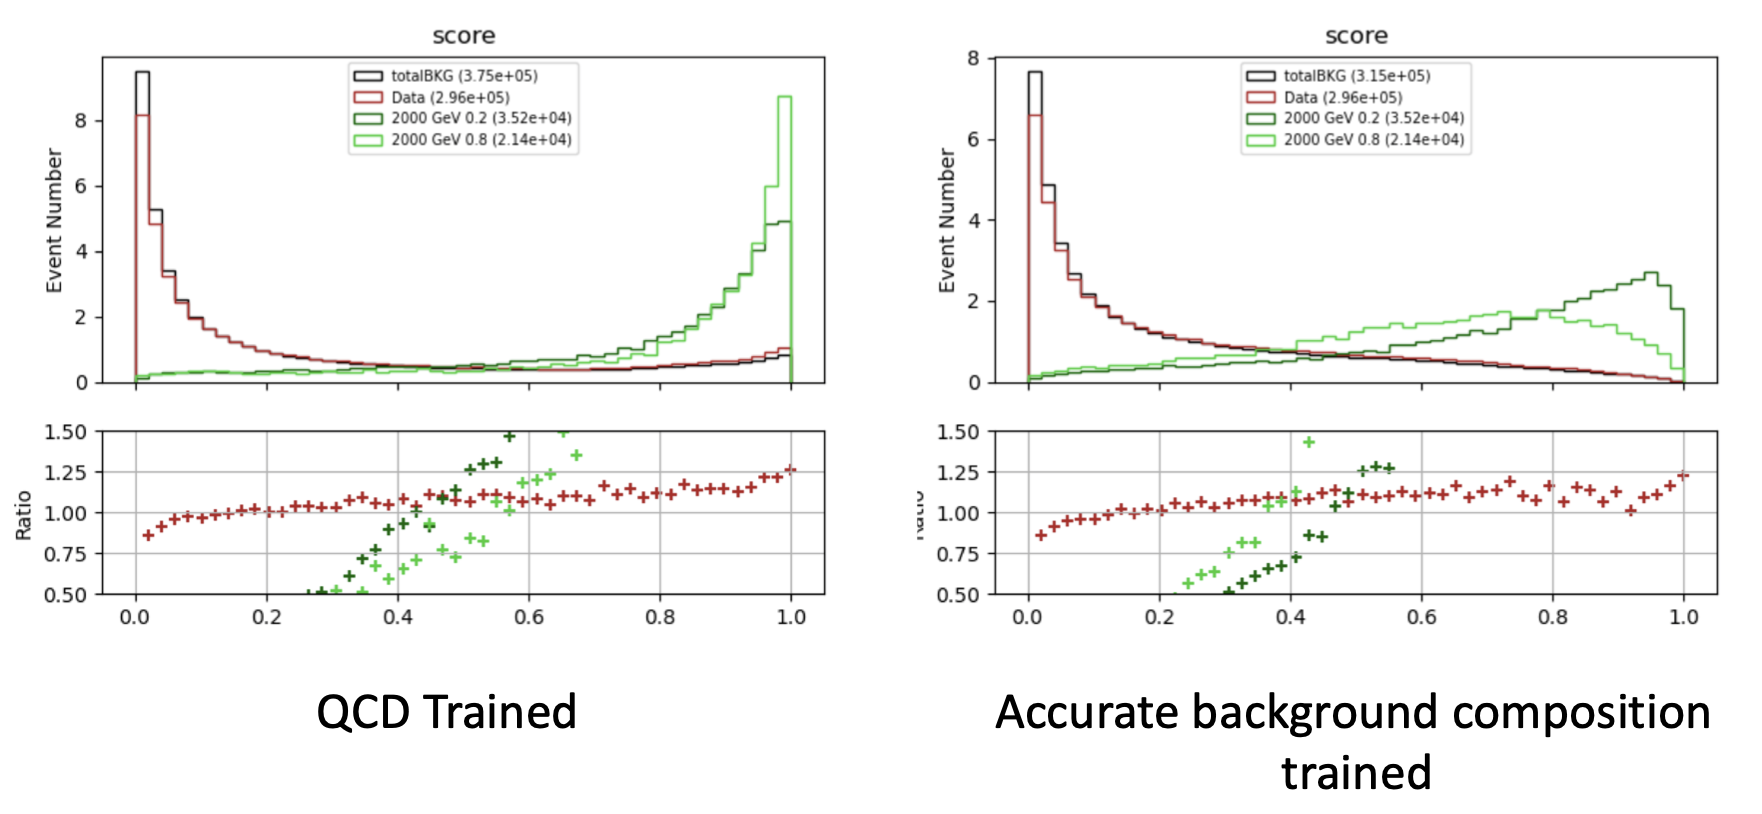
\includegraphics[width=0.98\textwidth]{figures/ml/pfn_MC_training_mixture}
    \caption{PFN score for full-background MC (black), data (red), and 2 representative signal points (green). The left plot is from a QCD-only training, while the right plot is from a full-background training. The histograms have been normalized to visualize the shapes better - the actual number of plotted events is shown in the legend. In the left plot we observe that both signal points are strongly classified as signal-like. In the right plot we observe less background contamination in the high score region, but worse signal classification. Both PFN trainings were tested for their effect on the analysis sensitivity and the QCD-only training was found to be favorable. 
    \label{fig:pfn_MC_training_mixture}}
\end{figure}

500k QCD MC background events and 500k SVJ signal events are used to train the network. The network is trained for 100 epochs. 20\% of the training events are used for training validation. Figure~\ref{fig:pfn_loss} shows the loss during training, which is stable and shows no indication of overtraining, and the final score that provides signal-background discrimination.

\begin{figure}[!htbp]
\centering
   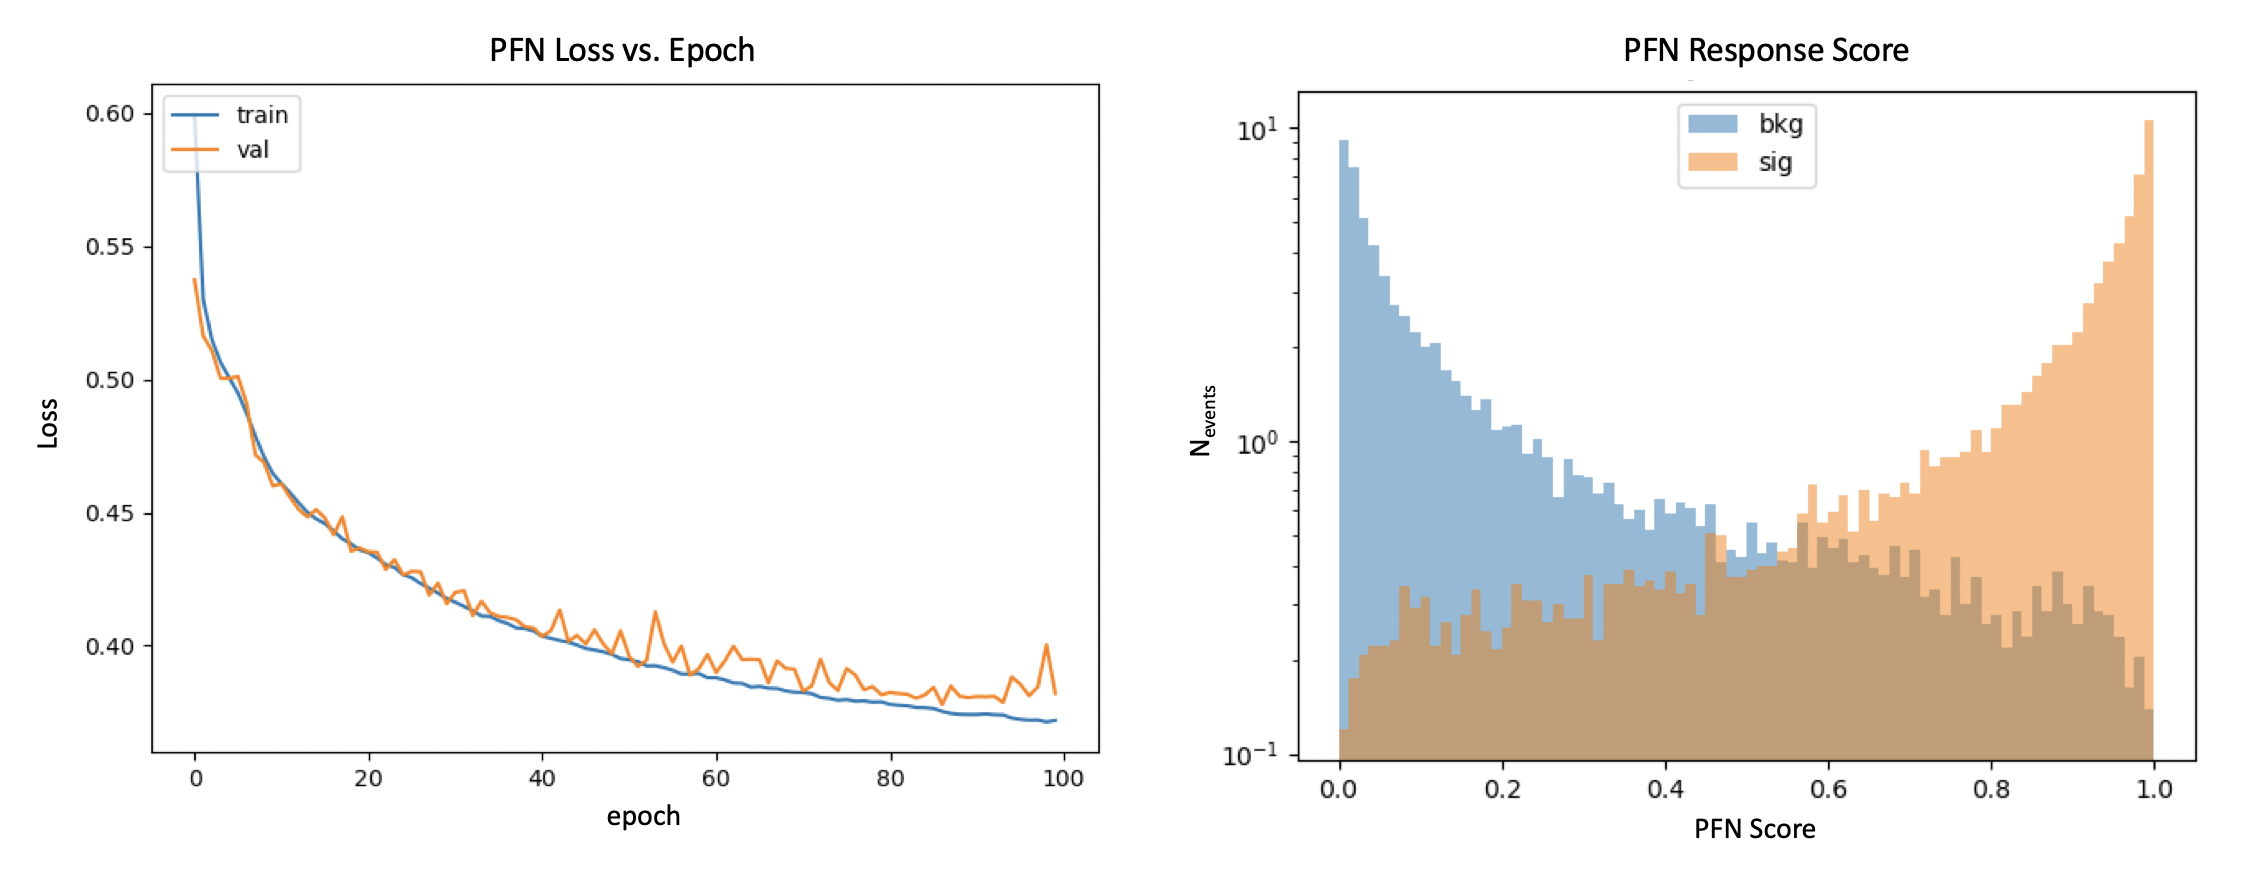
\includegraphics[width=0.9\textwidth]{figures/ml/pfn_loss_score}    
    \caption{PFN architecture loss during training as a function of epoch (left) and the evaluated score for signal and background training samples (right). The loss vs. epoch plot shows that the network is not overtrained. The score plot shows a good separation between signal and background.
    \label{fig:pfn_loss}}
\end{figure}

Optimization studies were performed on the PFN, varying the number of training epochs, number of training events, learning rate, number of nodes, and dimension of the $\Phi$ basis. A summary of these studies is presented in Appendix~\ref{app:pfn_qp}. The model presented here represents an optimal choice across these parameters.

%--------------------
\subsection{Performance}
\label{sec:pfn_performance}

The performance of the PFN is assessed via the AUC for each SVJ signal point.
Although the PFN is trained against QCD MC only, the performance is evaluated using data as the background sample, since the ultimate task of the PFN is to separate SVJ signals from data, which is dominated by SM processes.

Figure~\ref{fig:pfn_roc} shows the ROC curve of one such signal point, illustrating a smooth response.
Figure~\ref{fig:pfn_AUC_score_grid} shows the AUC of the PFN across the SVJ signal grid, demonstrating that AUC $>0.5$ is satisfied for all SVJ signals.

\begin{figure}[!htbp]
\centering
   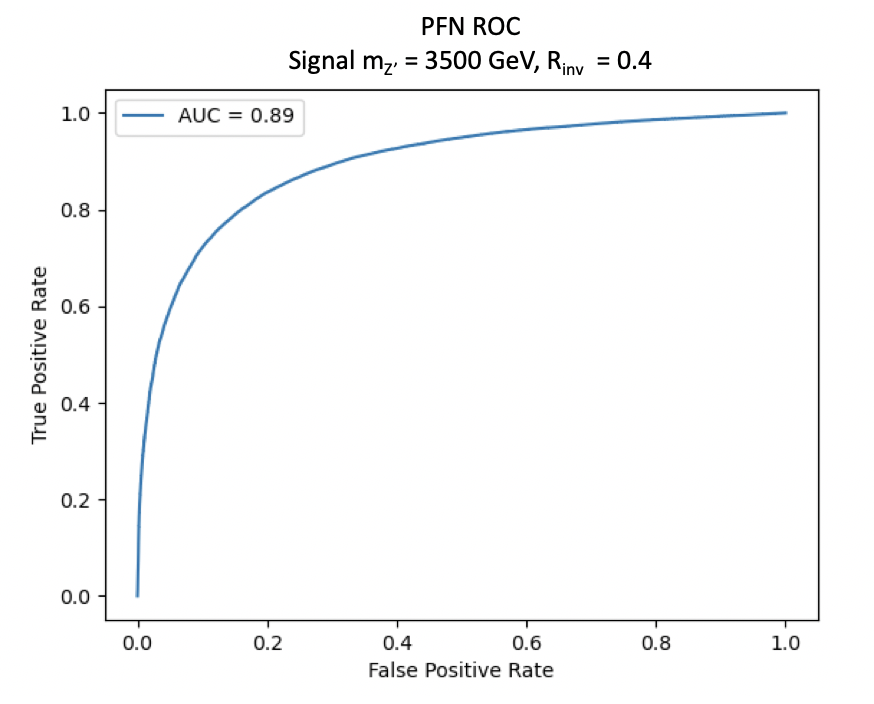
\includegraphics[width=0.7\textwidth]{figures/ml/pfn_roc}
    \caption{ROC for the PFN, using SVJ signal events (true positive) and data (false positive).
    \label{fig:pfn_roc}}
\end{figure}

\begin{figure}[!htbp]
\centering
   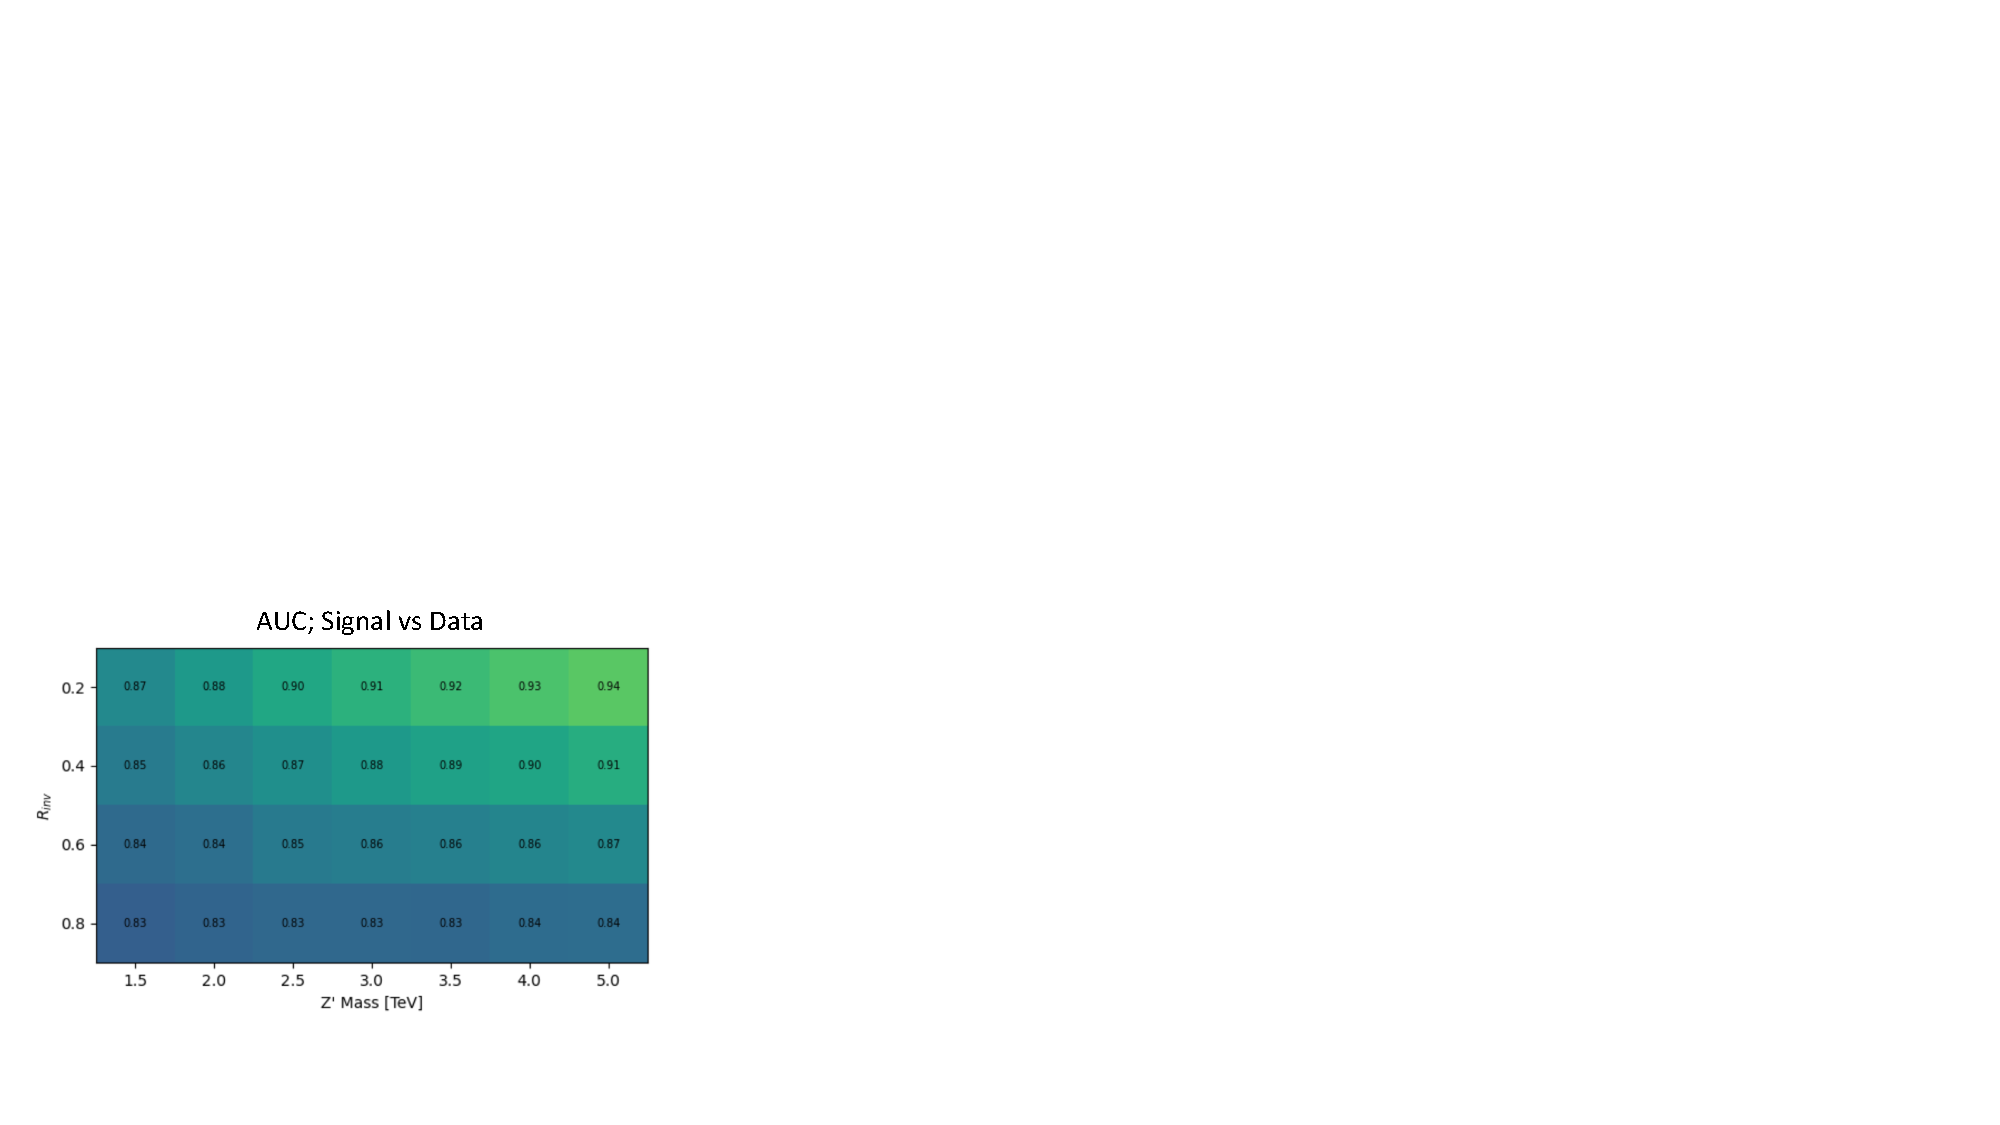
\includegraphics[width=0.7\textwidth]{figures/ml/pfn_AUC_grid}
    \caption{AUC for the PFN, shown for each signal in the SVJ grid.
    \label{fig:pfn_AUC_score_grid}}
\end{figure}

Figure~\ref{fig:pfn_score_all} shows the output score distribution for data and four signals, illustrating the range of scores received by data events in comparison to signal events.
As expected, most data events receive a background-like score (close to 0.0), indicating that the data is dominated by SM processes consistent with the background.
Most signal events receive a signal-like score (close to 1.0).
An optimization procedure determined that a selection of \textbf{PFN score > 0.6} can improve signal sensitivity across the grid.
The optimization procedure considered the cut that would maximize sensitivity as measured by $s/\sqrt{b}$, where $s$ the number of signal events accepted and $b$ is the number of background events selected.
This score selection is incorporated into the analysis design described in Chapter~\ref{ch:analysis}. 

\begin{figure}[!htbp]
\centering
   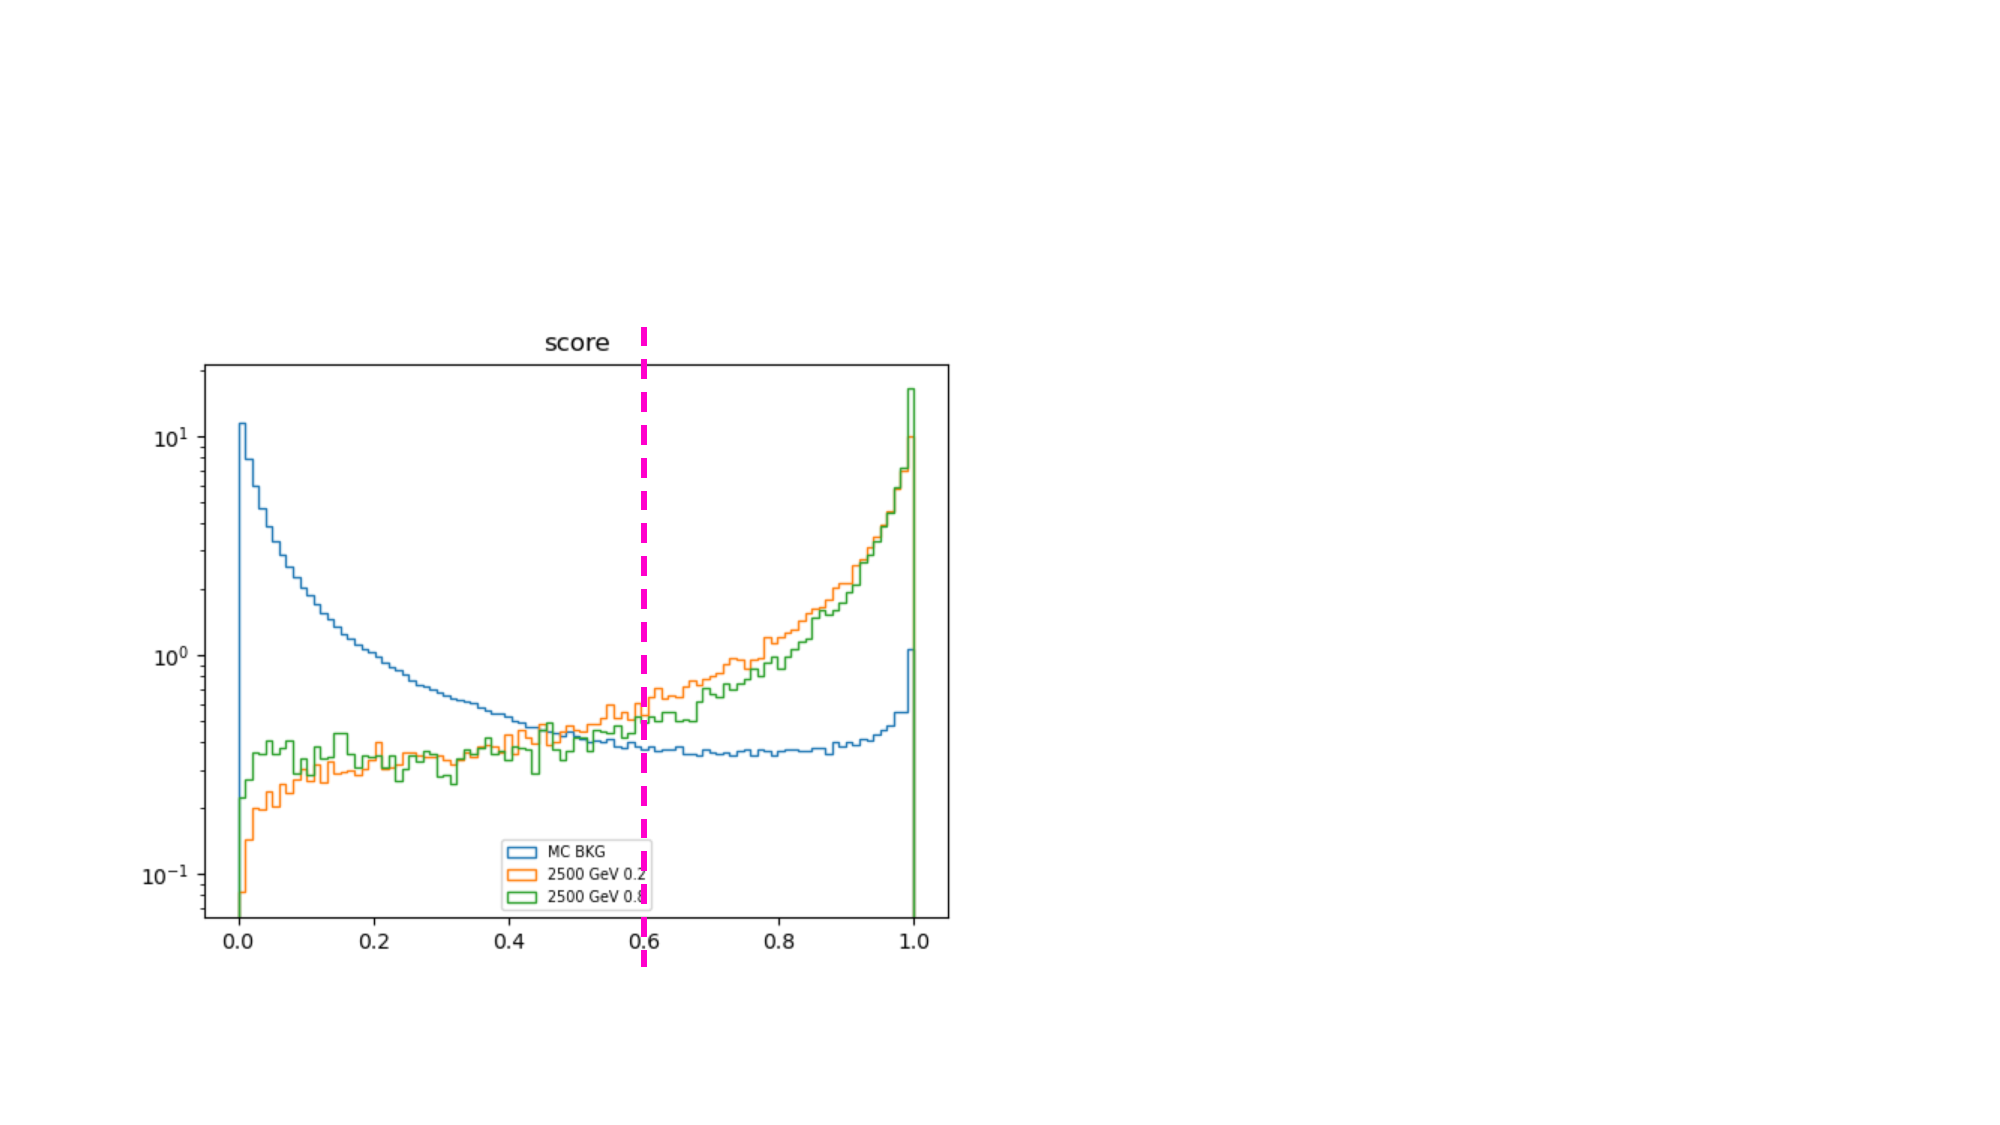
\includegraphics[width=0.5\textwidth]{figures/ml/pfn_score_all}
   \caption{Illustration of the PFN score selection, showing the separation between data (black) and 4 signal points (blue and green). The legend information takes the form ``$m_{Z'}$ \rinv'' for the signal. The PFN score selection value is shown by the pink line. Only events with a score > 0.6 will be accepted for use in the analysis. We see that most background (data) is rejected, while most signal is accepted.}
   \label{fig:pfn_score_all}
\end{figure}

%The agreement between data and background MC is illustrated in Figure~\ref{fig:mlscore_effComp}. The agreement is generally good, although some slope is observed in the ratio between the two shapes. The data has a small bias towards higher PFN scores compared to the background MC. However, the PFN score is only used in the analysis to make a selection on data events (PFN score > 0.6). The difference in selection efficiency for data and background MC <5.0\%, which is negligible for this analysis. 
%\begin{figure}[!htbp]
%\centering
%   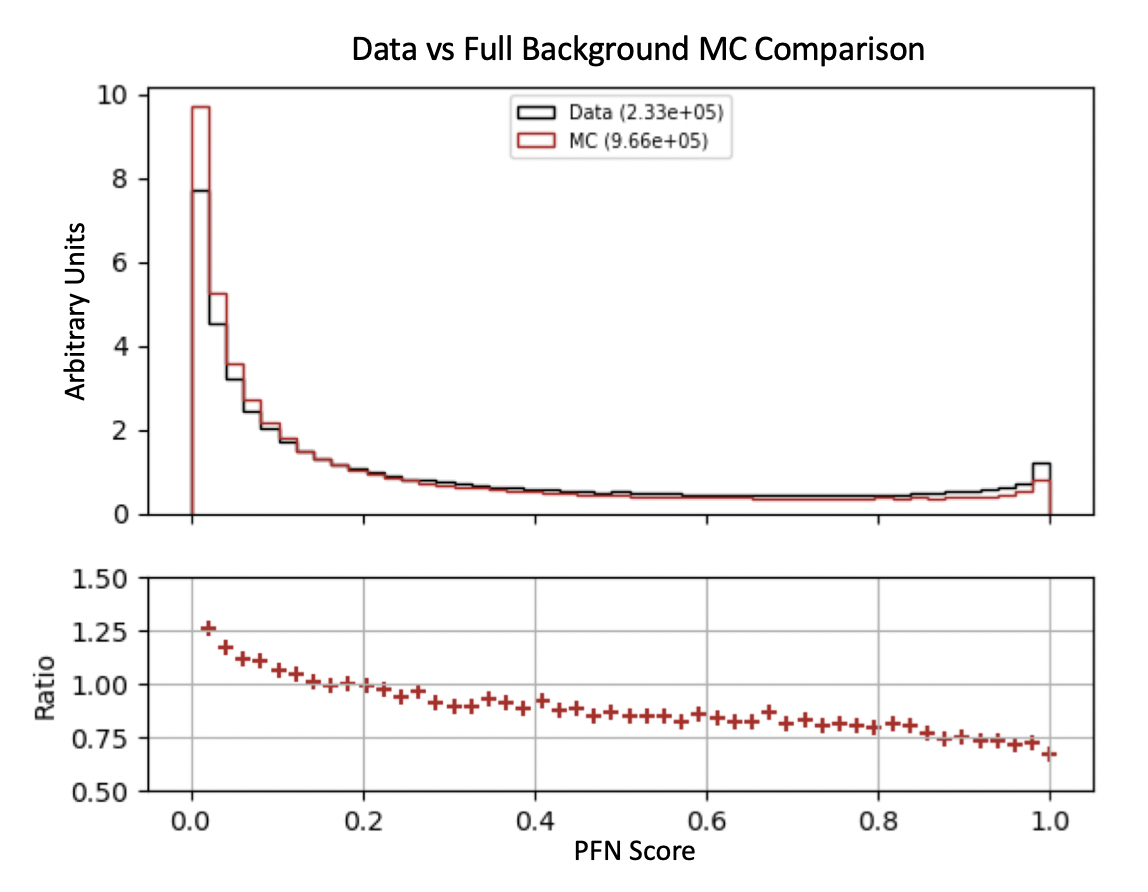
\includegraphics[width=0.5\textwidth]{figures/ml/mlscore_effComp}
%    \caption{PFN score comparison between normalized data and background MC shapes. Some slope is observed in the ratio panel.
%    \label{fig:mlscore_effComp}}
%\end{figure}

\clearpage


\section{ANTELOPE (Semi-supervised)}
\label{subsec:unsupervised}

The semi-supervised machine learning approach broadens the discovery potential of the search through the use of data-driven training, where no signal model is provided.
While broad sensitivity is a general goal of LHC searches, it is particularly motivated in the case of dark QCD models, which can lead to widely varying topologies depending on the values of model parameters.

%--------------------
\subsection{Architecture Fundamentals}
The model-independent search region of this analysis is implemented with a novel ML approach that builds on the PFN architecture to construct a tool that is capable of performing low-level anomaly detection with permutation-invariant inputs.
This tool, referred to as \textbf{ANomaly deTEction on particLe flOw latent sPacE (ANTELOPE)}, is a custom solution designed for this analysis.

Figure~\ref{fig:antelope_arch} provides a diagram of the ANTELOPE architecture. ANTELOPE uses the trained PFN network described in the previous section to generate a permutation invariant event representation $\mathcal{O}$ from track level inputs. The $\mathcal{O}$ basis is used as the input for a \textit{variational autoencoder} (VAE). A VAE is a common variation of a standard AE; the AE becomes \textit{variational} if the latent space is constructed through Gaussian sampling rather than a vector of weights, as described further in Ref.~\cite{vae2}. VAEs have been used in previous ATLAS searches to model low-level particle information, such as the search presented in Ref.~\cite{yxh} which used the recurrent architecture described in Ref.~\cite{vrnn}. One of the limitations of a recurrent architecture is the need to order the low-level inputs, which affects the performance of the tool. Jet track information is intrinsically unordered, and therefore a permutation invariant approach removes this element of arbitrary decision making from the modeling process. 

\begin{figure}[!htbp]
\centering
   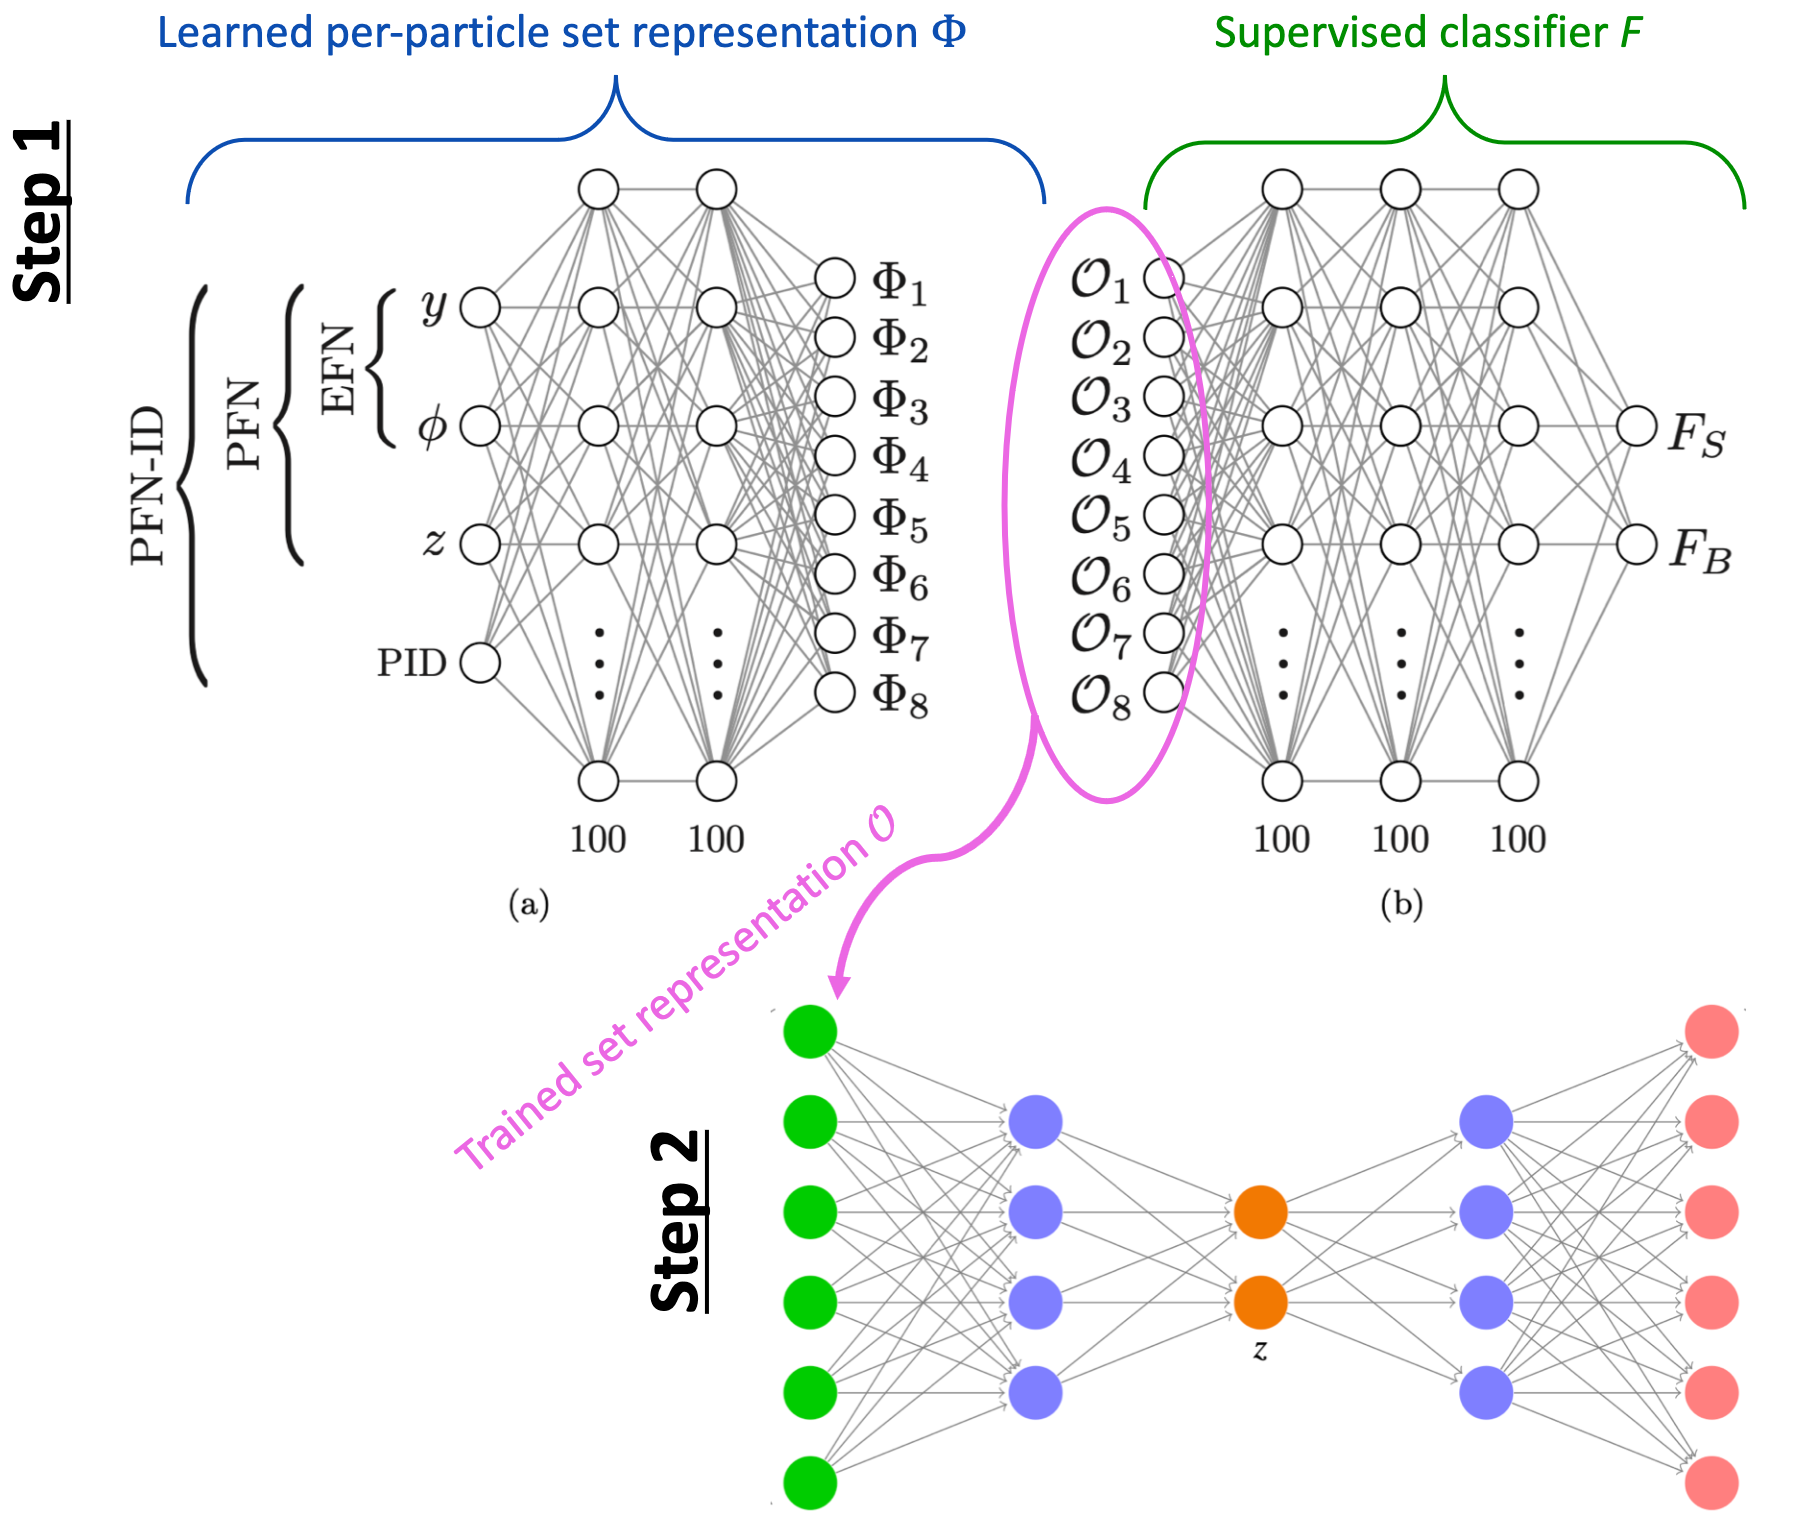
\includegraphics[width=0.9\textwidth]{figures/ml/antelope_arch}
    \caption{An annotated diagram of the ANTELOPE architecture. Step 1 illustrates the PFN which is fully trained before its use in the ANTELOPE network. Step 2 illustrates the variational auto-encoder. The Gaussian sampling of the latent space is shown, illustrating how the VAE differs from the AE shown in Figure~\ref{fig:ae}. 
    \label{fig:antelope_arch}}
\end{figure}

The input to ANTELOPE architecture is the same 6 track variables for the leading two jets, as presented in Section~\ref{sec:input_model}. The track information is encoded to the PFN $\mathcal{O}$ event representation using the pre-trained $\Phi$ neural network (trained according to the steps outline in Section~\ref{sec:pfn_training}). The VAE is then trained in an \textit{unsupervised} way using inputs encoded to $\mathcal{O}$ from data events only. Here \textit{unsupervised} means that the VAE is given no knowledge of the signal model during training. There is implicit knowledge of the signal model in the $\mathcal{O}$ encoding, so the full ANTELOPE network is considered semi-supervised, while the VAE component is unsupervised. A visual example of the $\mathcal{O}$ input to the VAE portion of the ANTELOPE is given in Figure~\ref{fig:antelope_input_rep}. 

\begin{figure}[!htbp]
\centering
   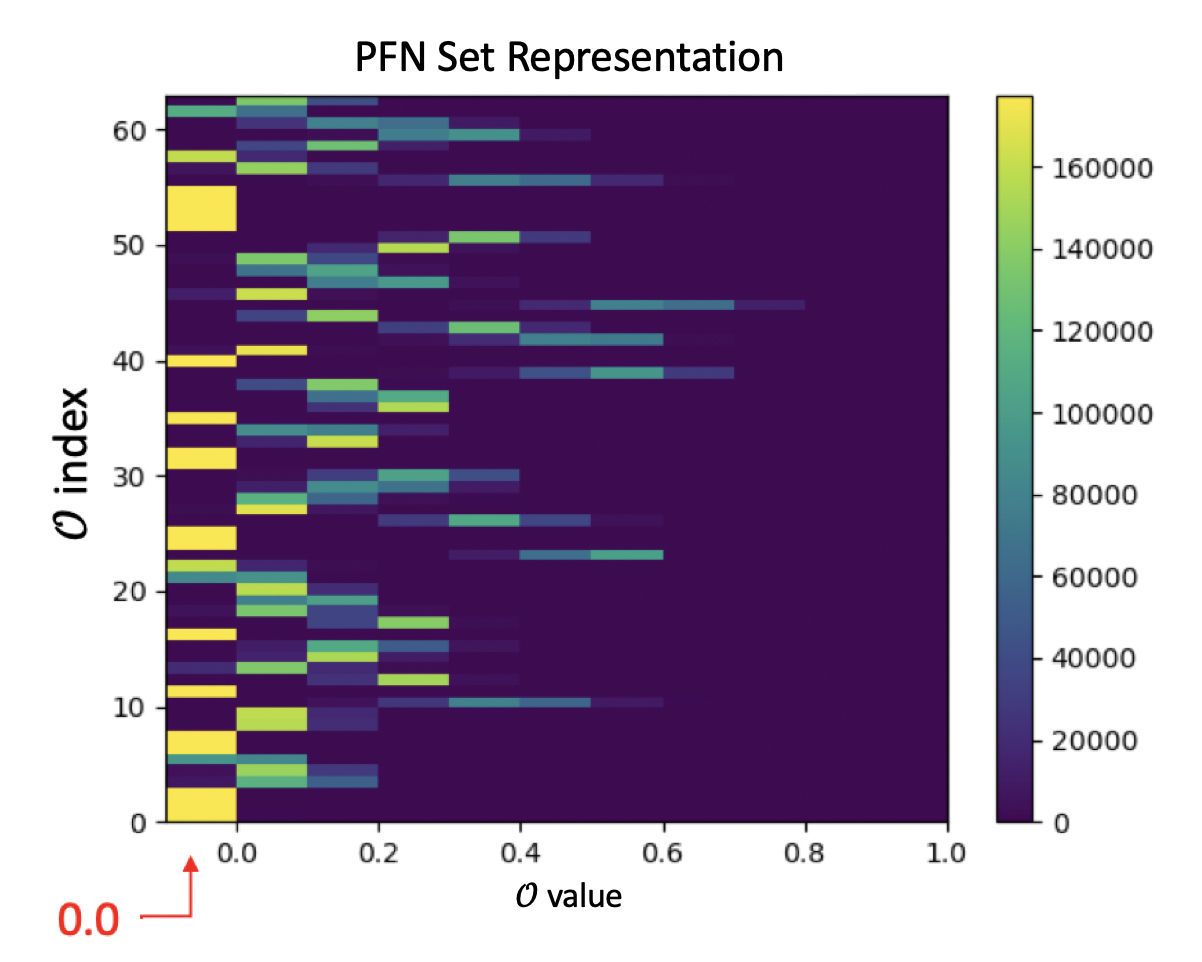
\includegraphics[width=0.7\textwidth]{figures/ml/antelope_input_rep}
    \caption{A visual representation of the 64 PFN $\mathcal{O}$ which create the input for the VAE component of ANTELOPE. The plot is 2D histogram of the PFN $\mathcal{O}$ index (0-63) versus the value assumed by that index. Many entries have a $\mathcal{O}$ value of exactly 0.0. To visually separate these from entries with a small but non-zero $\mathcal{O}$ value, any entries with value = 0.0 are moved to value = -0.01 (leftmost column) for the purpose of the plot only.
    \label{fig:antelope_input_rep}}
\end{figure}

The VAE is trained to minimize the reconstruction error, or the difference between its input and output layer. This pushes it to uncover patterns in the data, which is predominantly composed of SM processes. Any rare events in the data which present patterns inconsistent with the majority of the data will receive a higher reconstruction error. This error is used to create the anomaly score. 

%--------------------
\subsection{Training}

The VAE stage of the ANTELOPE network is trained over 500k data events.
The input dimensionality of the VAE has to match the encoded $\Phi$ dimension of the PFN, in this case 64. 
The encoding portion of the VAE has a hidden layer with 32 nodes,  and a latent space dimension of 12.
The decoding portion has another hidden layer of 32 nodes, and the output layer has a dimension of 64 to match the input layer.
All layers use a \textsc{relu} activation~\cite{scikit-learn} except for the output layer which uses a \textsc{sigmoid} activation~\cite{scikit-learn}, to restrict the output between 0 and 1.
As in the PFN, the Adam optimizer~\cite{adam}~\cite{scikit-learn} is used.

The network is trained for 50 epochs, with a learning rate of 0.00001. 
The VAE was observed to need a very small learning rate to effectively minimize the loss.
The loss $\mathcal{L}$ is the sum of two terms, the mean-squared error (MSE) of input-output reconstruction, and the Kullback-Leibler divergence (KLD).

\begin{equation}
\label{eq:vrnnloss}
\mathcal{L} = \sum_i L_i = \sum_i | \Phi_i^2 - \Phi\prime_i |^2 + \lambda D_{\text{KL}}
\end{equation}

Figure~\ref{fig:antelope_loss} shows the loss during training.
The validation events are seen to have a lower loss than the training events, indicating there is no issue with overtraining.
\begin{figure}[!htbp]
\centering
   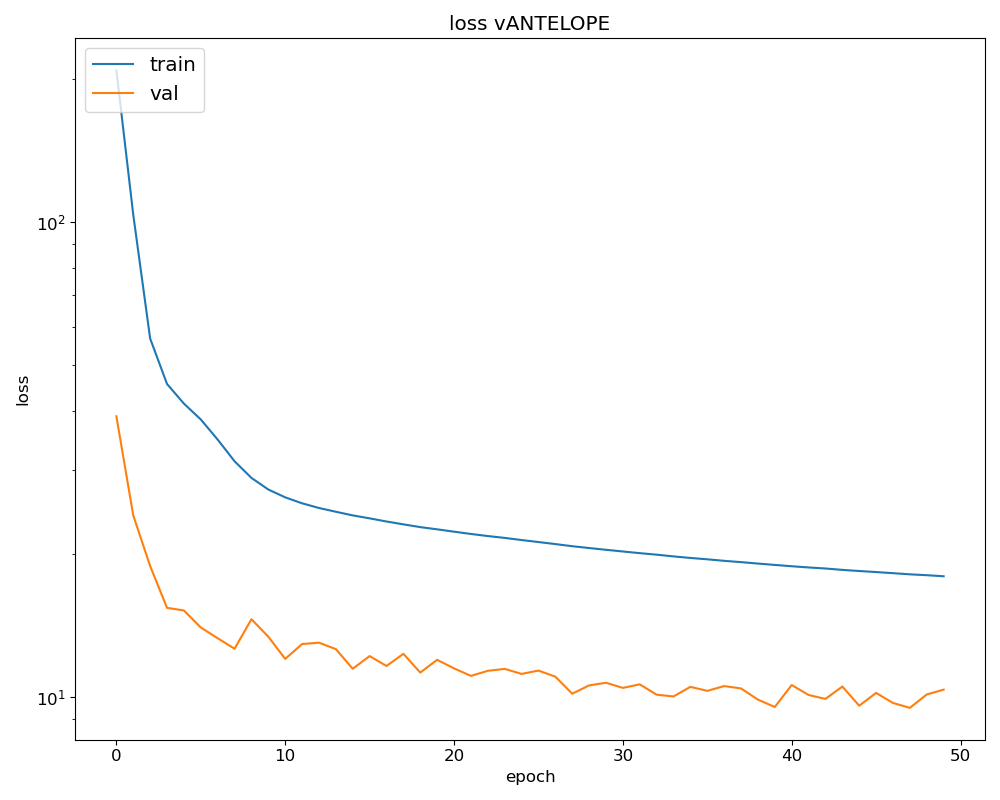
\includegraphics[width=0.5\textwidth]{figures/ml/antelope_loss}    
    \caption{ANTELOPE architecture loss during training as a function of epoch.
    \label{fig:antelope_loss}}
\end{figure}


%--------------------
\subsection{Performance}
\label{subsec:antelope_perf}

As with the PFN, the ANTELOPE performance is assessed via the ROC and AUC. 
Figure~\ref{fig:antelope_score} shows the anomaly score and an example ROC curve.
The anomaly score is calculated from the loss as defined in \ref{eq:vrnnloss}.
The score is produced by applying a sigmoid function to the loss to restrict its output between 0.0 and 1.0:

\begin{equation}
\label{eq:asfunc}
a = \frac{1}{1+e^{-\mathcal{L}}}
\end{equation}
where $a$ is the anomaly score and $\mathcal{L}$ is the VAE loss. Because the loss is always positive, the sigmoid transformation effectively restricts the anomaly score range between 0.5 and 1.0. The anomaly score is observed to range between 0.6 and 1.0, as the reconstruction loss is always non-zero. Following a similar sensitivity optimization as presented for the PFN score selection in Section~\ref{sec:pfn_performance}, a selection of \textbf{anomaly score > 0.7} is chosen for use in the analysis.

\begin{figure}[!htbp]
\centering
   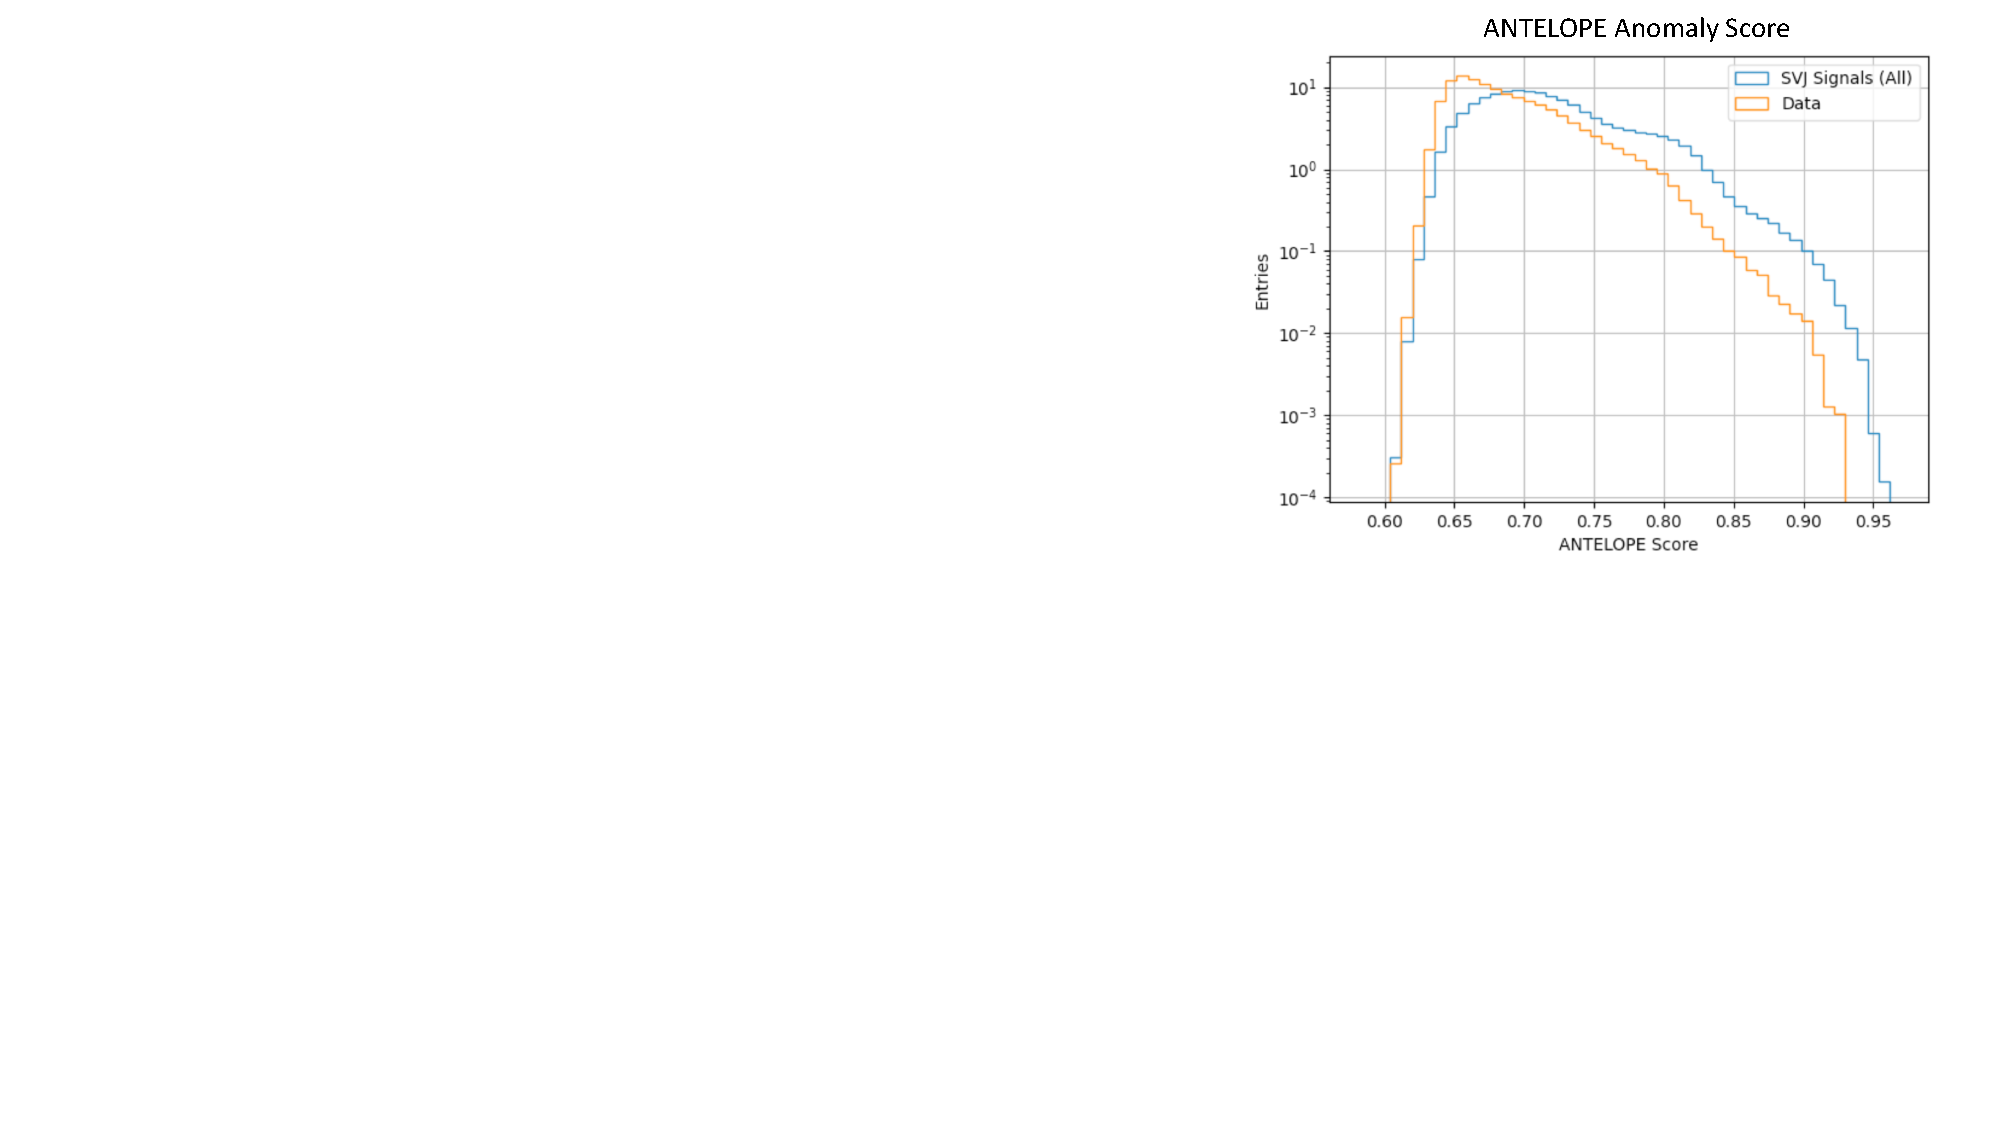
\includegraphics[width=0.48\textwidth]{figures/ml/antelope_score.pdf}
   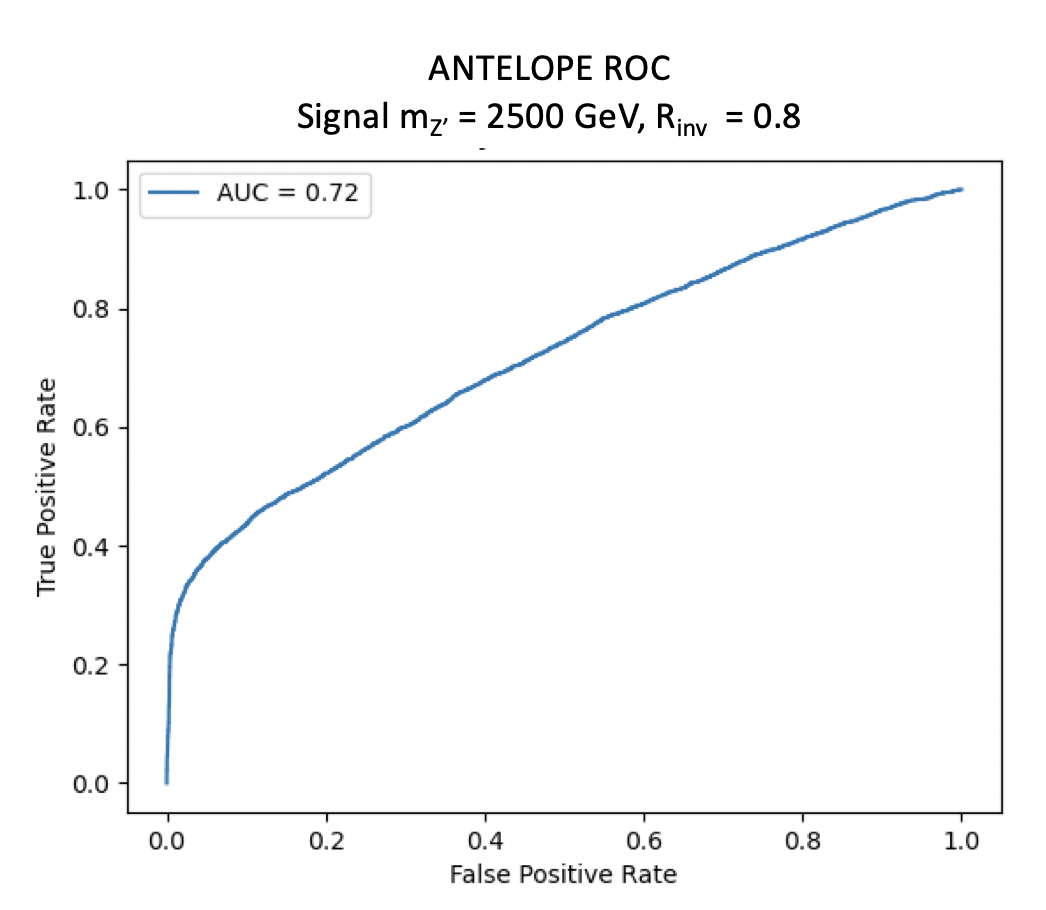
\includegraphics[width=0.48\textwidth]{figures/ml/antelope_roc}
    \caption{Anomaly score distribution (left), comparing all data (orange) and all SVJ signals (blue). The signals have a small but consistently higher score than the data, indicating that they are tagged as more anomalous by ANTELOPE. A ROC curve for an example signal point is also shown (right).
    \label{fig:antelope_score}}
\end{figure}

Figure~\ref{fig:antelope_AUC_score_grid} shows the AUC of the ANTELOPE across the SVJ signal grid, demonstrating discrimination capability across varying SVJ signal models.
Compared to the supervised PFN method, the ANTELOPE is not as performant (as expected due to the absence of signal model in training).
However, the network is seen provide separation between signal and background for all signal points, as evidenced by AUC $> 0.5$ across the signal grid.

\begin{figure}[!htbp]
\centering
   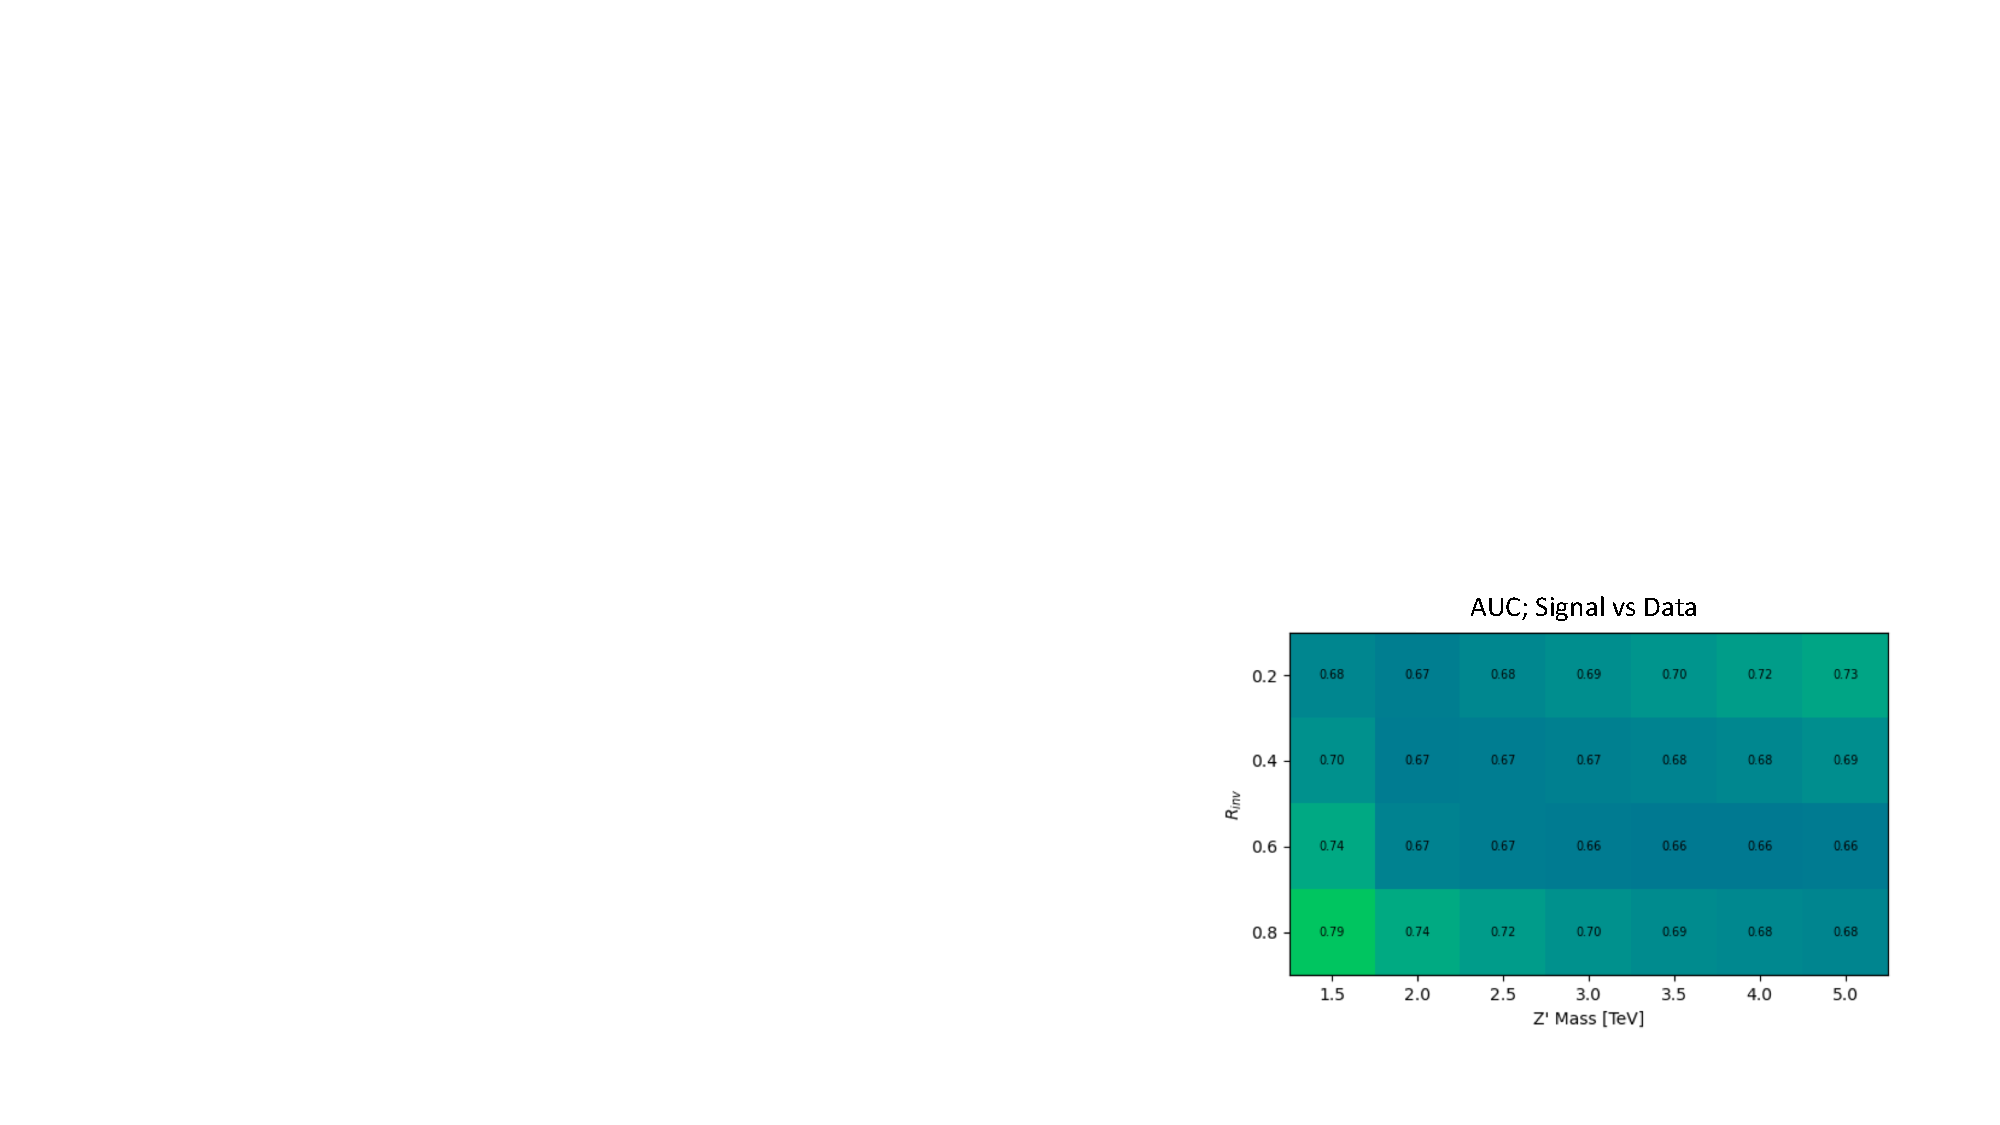
\includegraphics[width=0.7\textwidth]{figures/ml/antelope_AUC_score_grid}
    \caption{AUC from the ANTELOPE score for each signal in the SVJ grid.
    \label{fig:antelope_AUC_score_grid}}
\end{figure}

\paragraph{Model Independence} 

The unsupervised component of training the ANTELOPE network is expected to give it a more generalized sensitivity to new physics with \met~and jet activity, beyond the scope of the SVJ grid. 
To assess this, alternative signal models are evaluated with the trained ANTELOPE network.

The following alternate signal models were considered: 
\begin{itemize}
\item Z' $\rightarrow$ $t\bar{t}$ 
\item W' $\rightarrow$ WZ 
\item Gluino pair production $\rightarrow$ R-hadron + LSP (\met) with gluino masses 2000/3000 GeV, LSP mass 100 GeV, and lifetime 0.03 ns (LSP = \textit{lightest supersymmetric particle})
\item Emerging jets s-channel with mass 1000 GeV and lifetime 1ns 
\end{itemize}

Figure~\ref{fig:antelope_altsig} shows the distribution of these signals in the PFN score and the ANTELOPE anomaly score.
The benefit of the ANTELOPE in enhancing model independence is clearly seen through the boost in performance for certain non-SVJ signal models.
The gluino and emerging jet signals in particular are marked as highly anomalous by the ANTELOPE, but are marked as evenly background-like and signal-like by the PFN.
This observation demonstrates that the use of the ANTELOPE network in this analysis has the potential to expand our sensitivity to include alternate signal models that could be marked as highly anomalous with the anomaly score.

\begin{figure}[!htbp]
\centering
   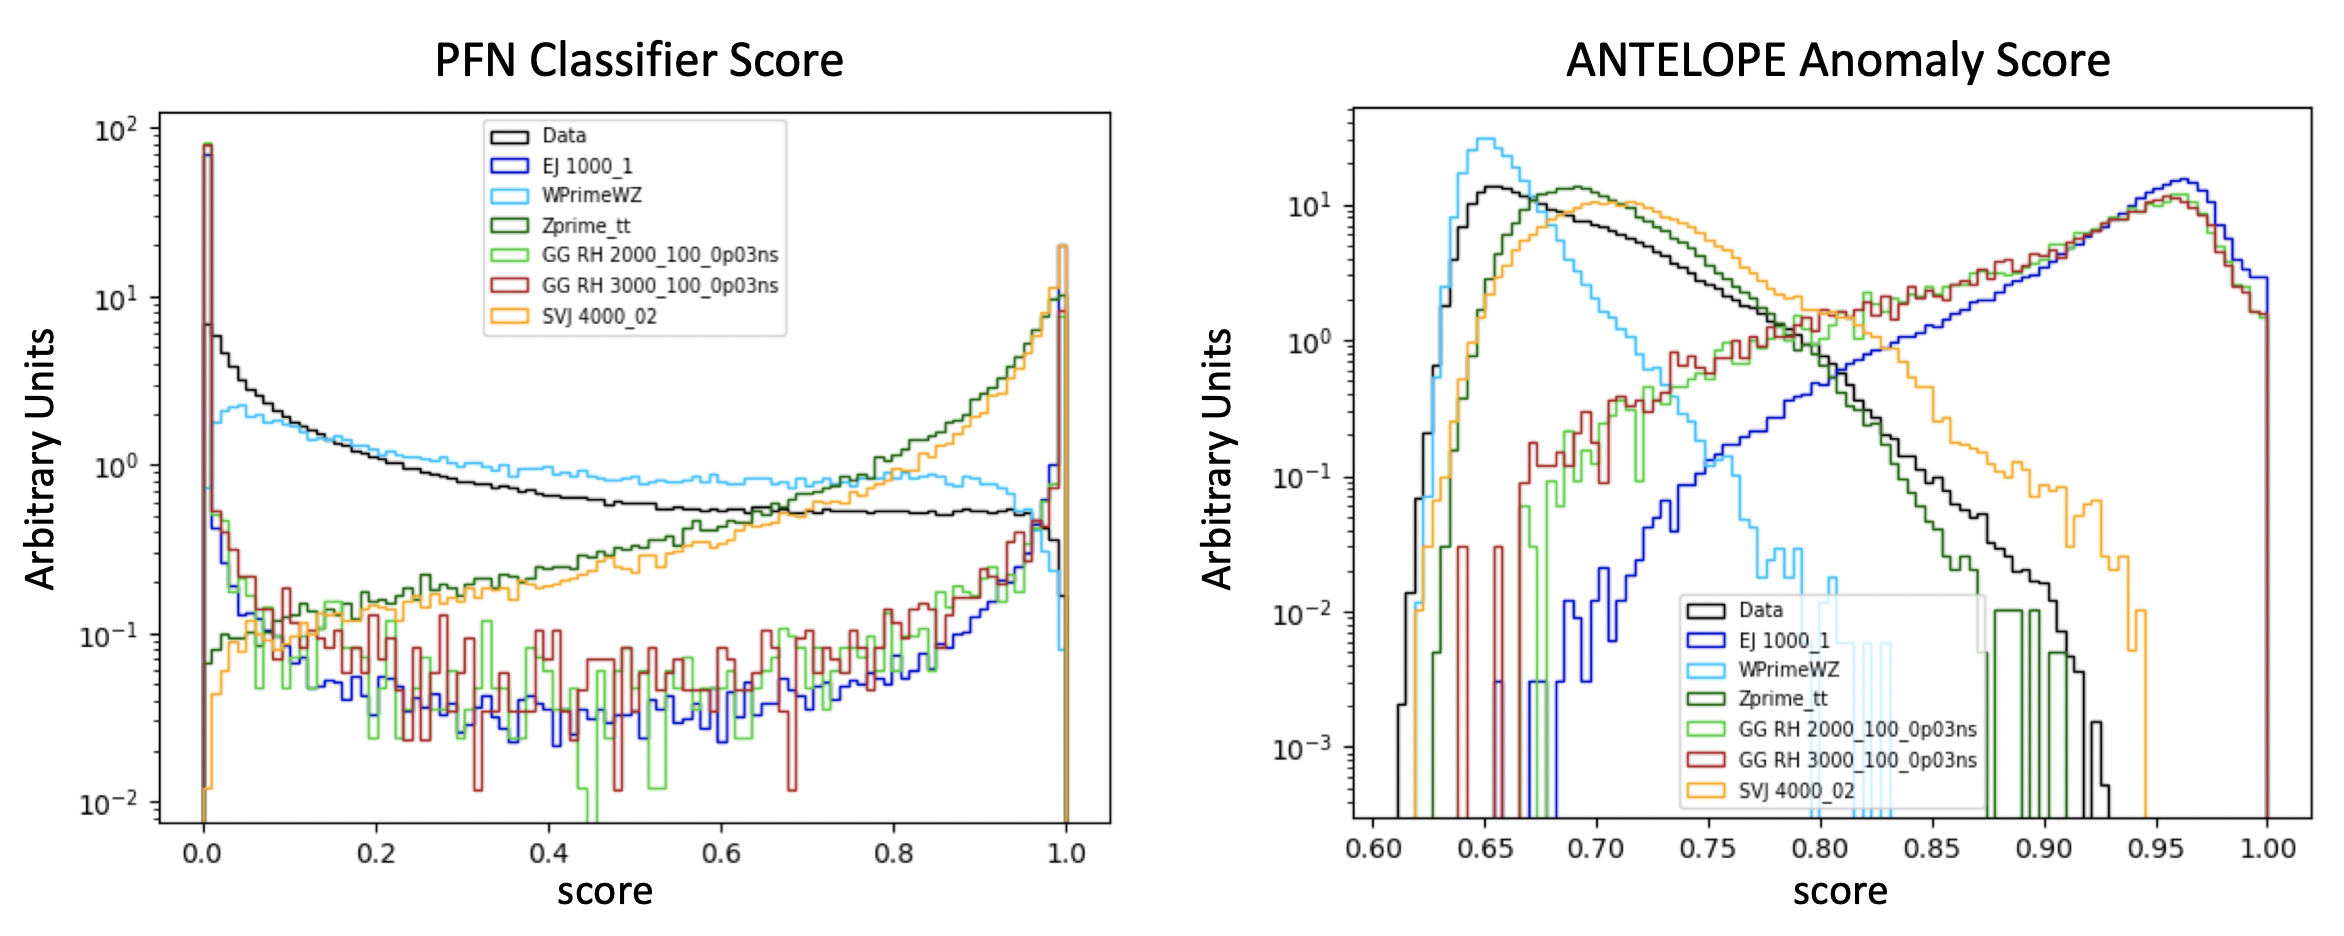
\includegraphics[width=0.98\textwidth]{figures/ml/antelope_vs_pfn_score}
    \caption{Comparing data and the alternate signal models for the PFN score (left) and ANTELOPE score (right). The emerging jet signal (dark blue) and gluino R-hadron signals (red, light green) are an example of the advantage of the model-independent ANTELOPE approach. These signals have a bimodal shape in PFN score but are clearly tagged with a high anomaly score by the ANTELOPE.
    \label{fig:antelope_altsig}}
\end{figure}







%%%%%%%%%%%%%%%%
% Chapter 8
%%%%%%%%%%%%%%%%
%\chapter{Analysis Strategy}
\label{ch:analysis}

This chapter will present the strategies used to isolate ATLAS data events most consistent with the SVJ model and to estimate the relevant background. The data and MC samples discussed in Chapter~\ref{ch:mc_data} are studied to create the analysis strategy, and the ML scores discussed in Chapter~\ref{ch:ml_tools} are used to isolate the most signal like events. The background is estimated from the \textit{transverse mass} (\mt) spectrum, which captures the main components of the $Z'$ decay. A \textit{preselection} selects events consistent with the SVJ topology based on basic features of the jets and \met. Preselected events are then split into a \textit{control region} (CR), \textit{validation region} (VR), and \textit{signal region} (SR). The CR and VR are used to validate the background estimation procedure. The SR is blinded during the development of the analysis strategy, and only unblinded to make the final measurements presented in Chapter~\ref{ch:results}. The final result is a polynomial fit of the \textit{transverse mass} (\mt) spectrum in the SR. The preselection, region definitions, and polynomial fit will be discussed in detail in the following sections.

\section{Transverse Mass}
\label{sec:mt}
The transverse mass \mt~is chosen as the search variable due to the potential for the SVJ signal to create a resonant shape around the mass of the $Z'$. \mt~is the total transverse mass of the two leading jets and the \met, expressed in Equation~\ref{eq:mt} as:

\begin{equation}
m_T^2 = [E_{T,jj} + \met~]^2 - [\vec{p}_{T,jj} + \vec{p}_T^{\text{miss}}]^2
\label{eq:mt}
\end{equation}

where $E_{T,jj}$ is the transverse energy of the dijet system. We take $E_{T,jj} = m_{jj}^2 + |\vec{p}_{T,jj}|^2$, where $m_{jj}^2$ is the invariant mass of the two leading jets, and $\vec{p}_{T,jj}$ is the vector sum of the \pt~of the two leading jets. \mt~is selected as the search variable in place of simpler invariant mass $m_{jj}$ because substantial energy from the Z' decay is captured in the \met~. Therefore incorporating \met~into \mt~improves the resonance around the mass of the $Z'$. \par

Figure~\ref{fig:mt_mass} illustrates the resonance in \mt~of the SVJ signals. The smoothly falling background is shown in comparison to the resonant shape of the signals, which form a peak just below the associated $Z'$ mass. The lower \rinv~signals form a more distinctive resonance in \mt, while the high \rinv~signals have a much wider \mt~shape.
\begin{figure}[!htbp]
\centering
    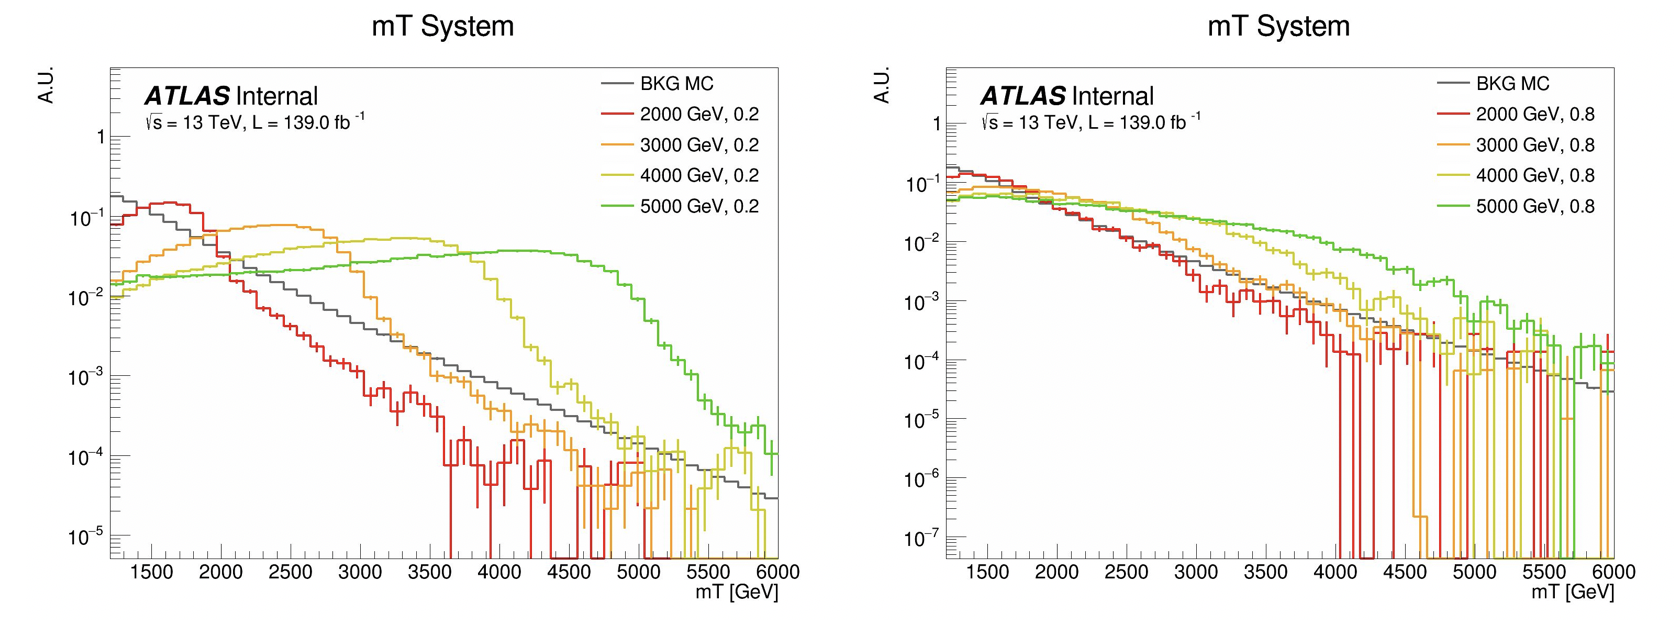
\includegraphics[width=0.98\textwidth]{figures/ch8/mt_mass_norm}
    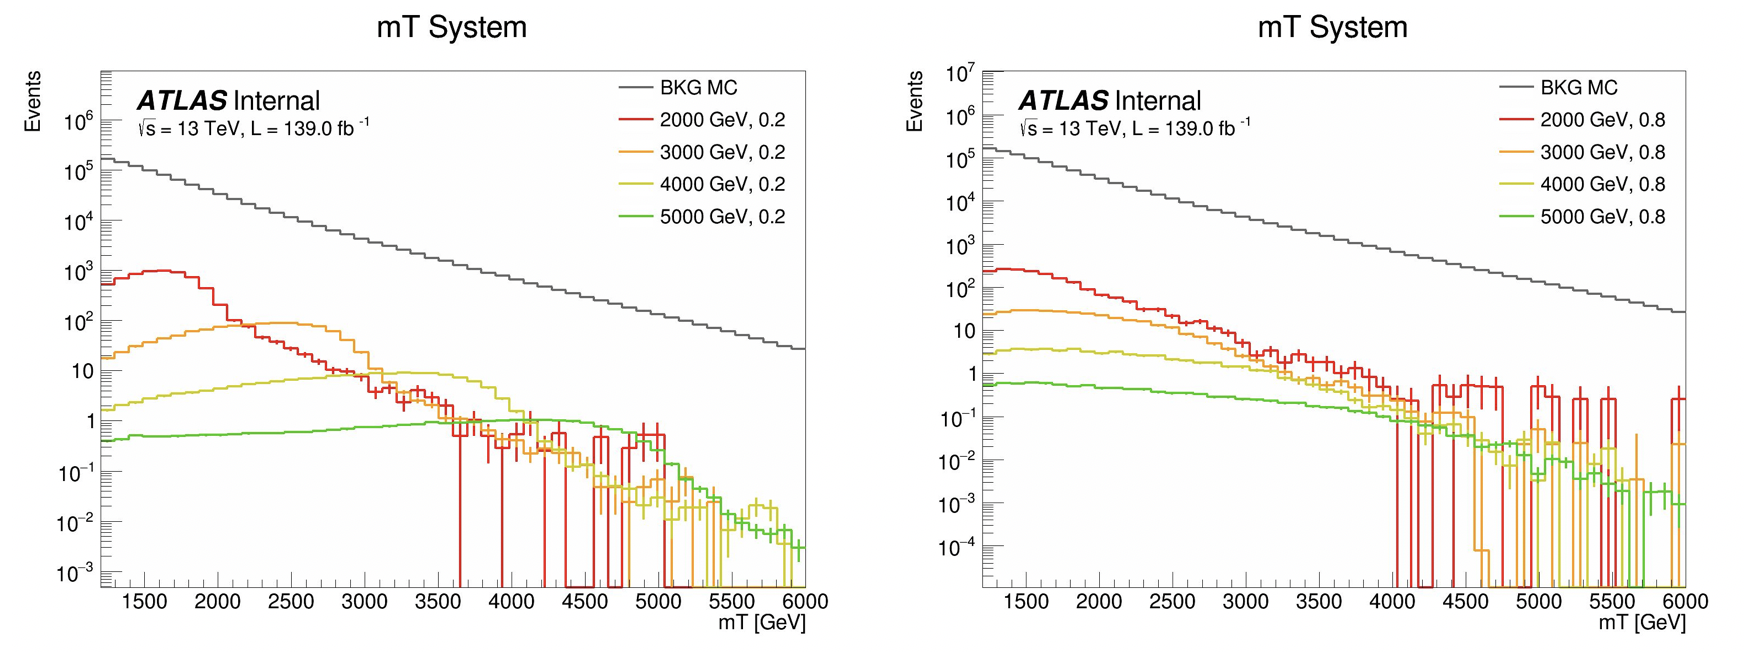
\includegraphics[width=0.98\textwidth]{figures/ch8/mt_mass_unnorm}
    \caption{The resonant shape of the SVJ signals (color) in \mt, in contrast to the smoothly falling \mt~background (grey). The top row illustrates unit normal shapes, so that the shape of the signals is more easily seen. The bottom row illustrates the signal and background scaled to their expected yield at preselection, illustrating the relative expected statistics. The \rinv~= 0.8 signals (right) boast a wider shape, making them more difficult to detect, while the \rinv~= 0.2 signals (left) produce a more narrow resonance in \mt~. The signal models are identified in the legend as ``$m_{Z'}$, \rinv''. 
    \label{fig:mt_mass}}
\end{figure}

%------------------------------------------------- 
\section{Preselection}
\label{sec:eventsel}

The preselection isolates the phase space of events that most closely match the SVJ signal topology. Each cut was determined to reduce the background and enhance signal sensitivity.
The list of preselection cuts and the motivation behind each cut are as follows. 
Here ``jets" refer to anti-$k_t$ R=0.4 jets, as discussed in Chapter~\ref{ch:part_reco}.

\begin{itemize}
\item At least 2 jets; in order to reconstruct the resonance mass
\item Leading jet ($j_1$) \pt $>$ 450 GeV; to ensure the trigger is fully efficient
\item Subleading jet ($j_2$) \pt $>$ 150 GeV; to mitigate the presence of non-collision background (Appendix~\ref{app:ncb})
\item $|\eta_{j1,j2}|$ $<$ 2.1; to ensure jets are fully within the tracker
\item $\Delta$Y$<$ 2.8 (difference in rapidity between $j_1$ and $j_2$); to ensure central production associated with the hard scatter  
\item \met $>$ 200 GeV; to restrict the phase space to events with possible dark particles 
\item \mt $>$ 1.2 TeV, to ensure a smoothly falling \mt~distribution for fitting (Section~\ref{sec:background})
\item At least 3 tracks for each of the two leading jets $j_1$ and $j_2$; to have adequate tracking information for the ML tools
\item $\Delta\Phi$($j_1$,$j_2$) $>$ 0.8; to mitigate the presence of non-collision background (Appendix~\ref{app:ncb}).
\end{itemize}

Table~\ref{fig:presel_cutflow} shows the impact of these cuts in sequence for data and signal.
\begin{table}[!htbp]
\centering
   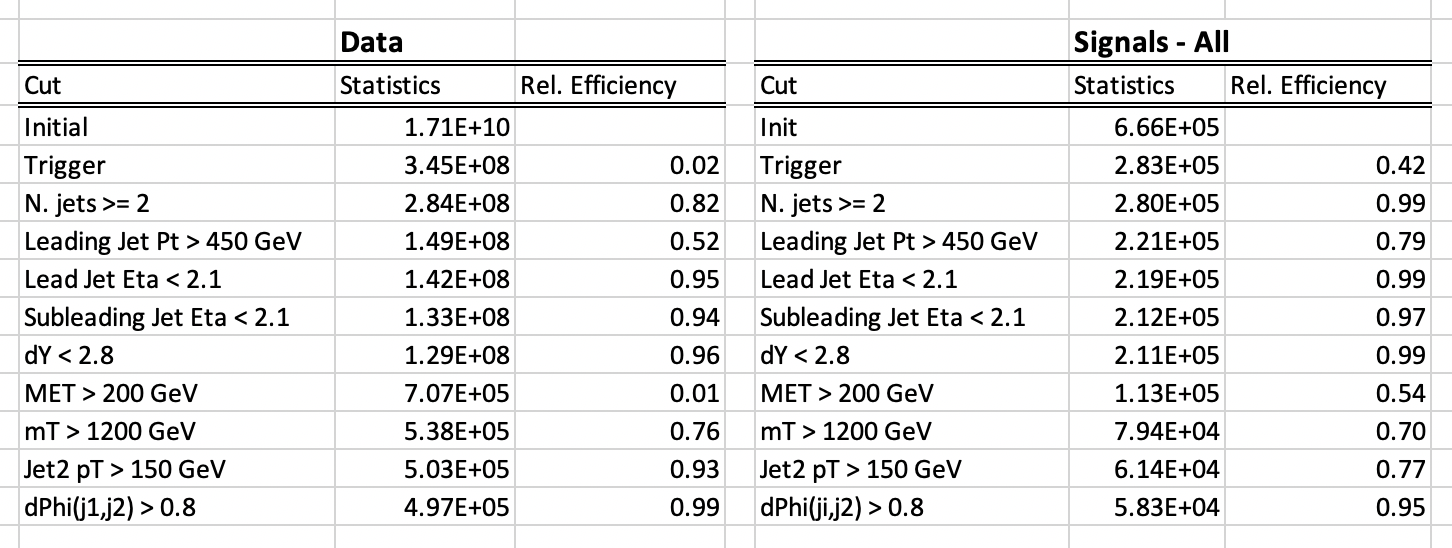
\includegraphics[width=0.95\textwidth]{figures/eventsel/preselection/presel_cutflow}
    \caption{Preselection cuts for data (left) and signal (right).
    \label{fig:presel_cutflow}}
\end{table}

With the exception of the cuts necessary to reduce the non-collision background, all cuts were verified to enhance signal sensitivity by improving $s/\sqrt{b}$, a standard estimate of discovery sensitivity, where $s$ is the number of signal events and $b$ is the number of background events. The cuts on $\Delta$Y and \met~were optimized to enhance $s/\sqrt{b}$, and the other cuts were informed by the physics motivations provided above. \par

Vetos are applied to reject any events where an error for a subdetector is flagged. 
To reject non-collision backgrounds (NCB), such as calorimeter noise, beam halo interactions, or cosmic rays, the standard ATLAS event cleaning procedure is applied.
As this analysis is very dependent on \met~associated to jets, the \textsc{Tight}~\cite{tight_loose} event cleaning working point is applied. 
Tight cleaning requires jets to pass a stricter set of quality requirements compared to the \textsc{Loose}~\cite{tight_loose} cleaning option.
Due to the alignment between jets and \met~ for SVJ events, it was found that two additional cuts (indicated above) are needed to remove NCB.
The process for selecting these cuts is presented in Appendix~\ref{app:ncb}. 

The leading and subleading jets in each event are considered the dark quark candidates from the $Z' \rightarrow q_D\bar{q_D}$ decay.  
They are therefore the two jets of greatest interest in the event, and used in the computation of key analysis variables.
This choice was determined through studies of the dark quark trajectory in simulation which determined that the leading and subleading jets are most often aligned with the dark quarks, and therefore most likely to capture the dark quark hadronization.
This study can be found in Appendix~\ref{app:truthstudies}.

Figure~\ref{fig:presel_vars} and Figure~\ref{fig:presel_vars2} show the distribution of signals, data and background MC in several key analysis variables after preselection is applied.
The variables illustrated are:
\begin{itemize}
\item Transverse mass \mt: key analysis variable which reconstructs the $Z'$ mass, as discussed in Section~\ref{sec:mt}.
\item Leading jet \pt: the trigger variable, and a component of \mt. 
\item Subleading jet \pt: dark quark candidate and component of \mt.
\item Missing transverse energy \met (or MET): component of \mt, and an indication of the presence of dark hadrons. All signals are observed to have more \met than the background.
\item $\Delta\phi$(j1, j2): difference in trajectory of the two leading jets, measured in the $\phi$ plane (recall the ATLAS detector geometry of Figure~\ref{fig:ATLASgeometry}). Orientation of the jets is of importance to the ML model as discussed in Section~\ref{sec:input_model}. 
\item $\Delta$Y(j1, j2): difference in trajectory of the two leading jets, measured in the Y plane (recall Figure~\ref{fig:ATLASgeometry} and the definition of rapidity Equation~\ref{eq:rapidity}). The signals are seen to have lower $\Delta$Y(j1, j2) than the background.
\item $\Delta\phi$(j1, \met): the angular separation between the leading jet and the \met. The leading jet is predominantly back-to-back with the \met.
\item $\Delta\phi$(j2, \met): the angular separation between the subleading jet and the \met. The subleading jet is predominantly aligned with the \met, which is a unique feature of this analysis as jets that are closely aligned with \met~are often removed from other ATLAS analyses.
\end{itemize}

\begin{figure}[!htbp]
\centering
    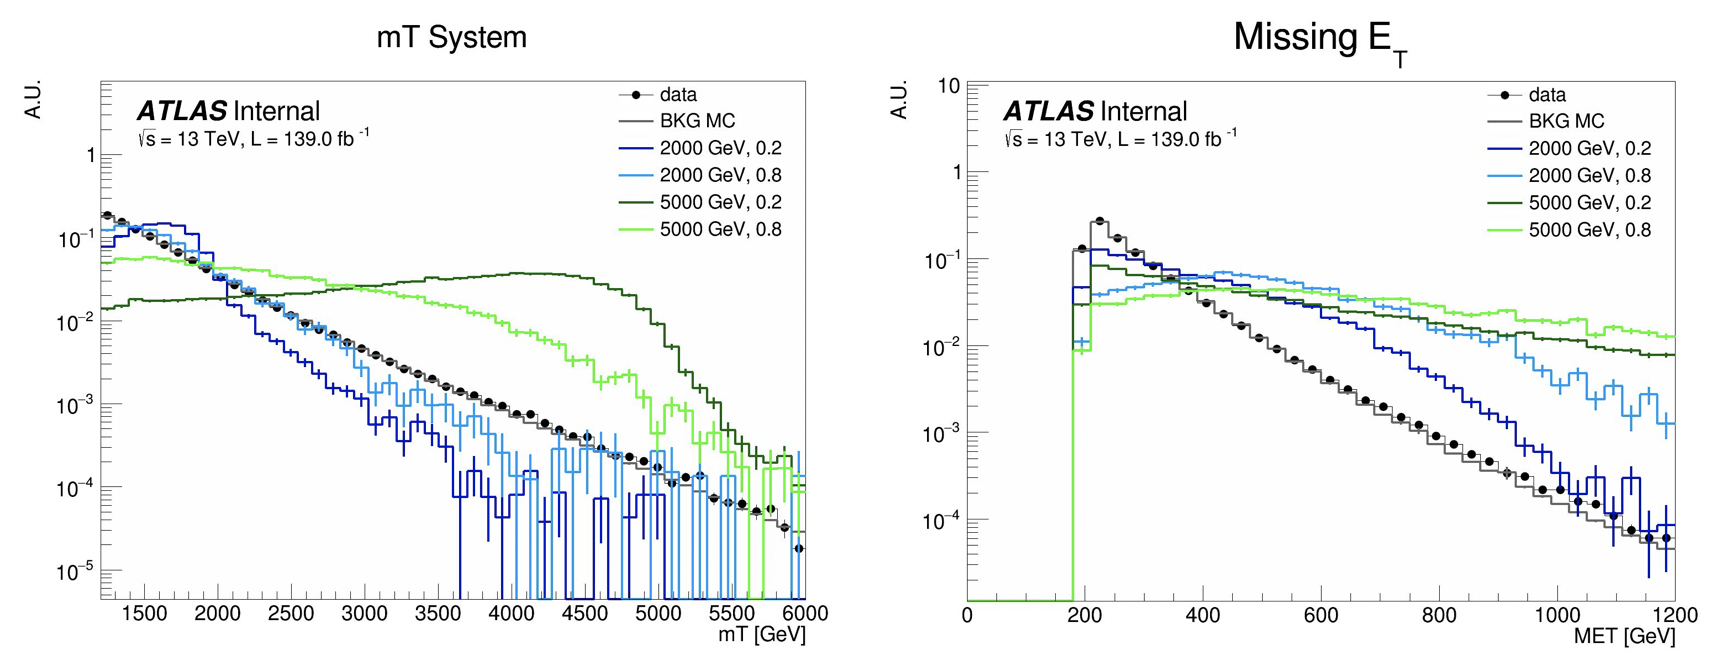
\includegraphics[width=0.95\textwidth]{figures/eventsel/preselection/presel1}
    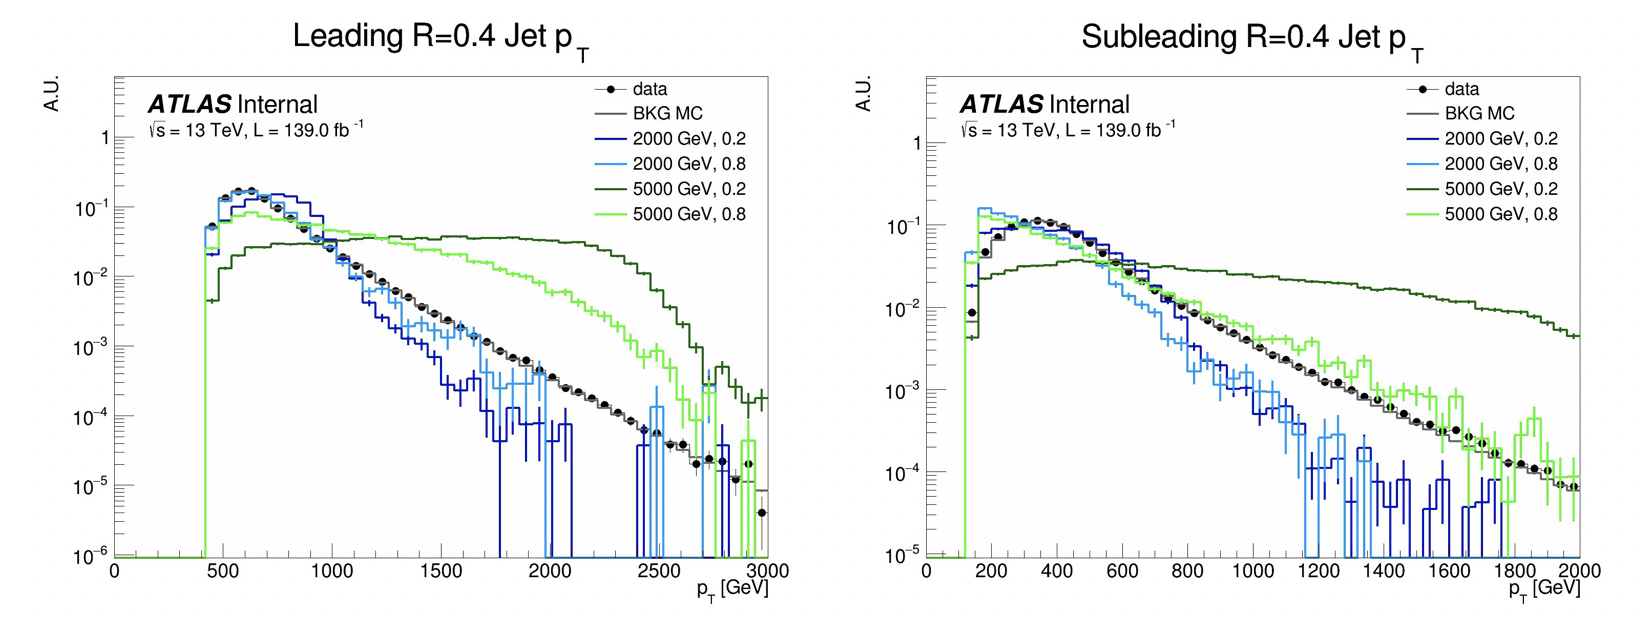
\includegraphics[width=0.95\textwidth]{figures/eventsel/preselection/presel2}
    \caption{Energy and momentum analysis variables at preselection, for data (black), background MC (grey), and representative signal models (color). The signal models are identified in the legend as ``$m_{Z'}$, \rinv''. 
    \label{fig:presel_vars}}
\end{figure}

\begin{figure}[!htbp]
\centering
    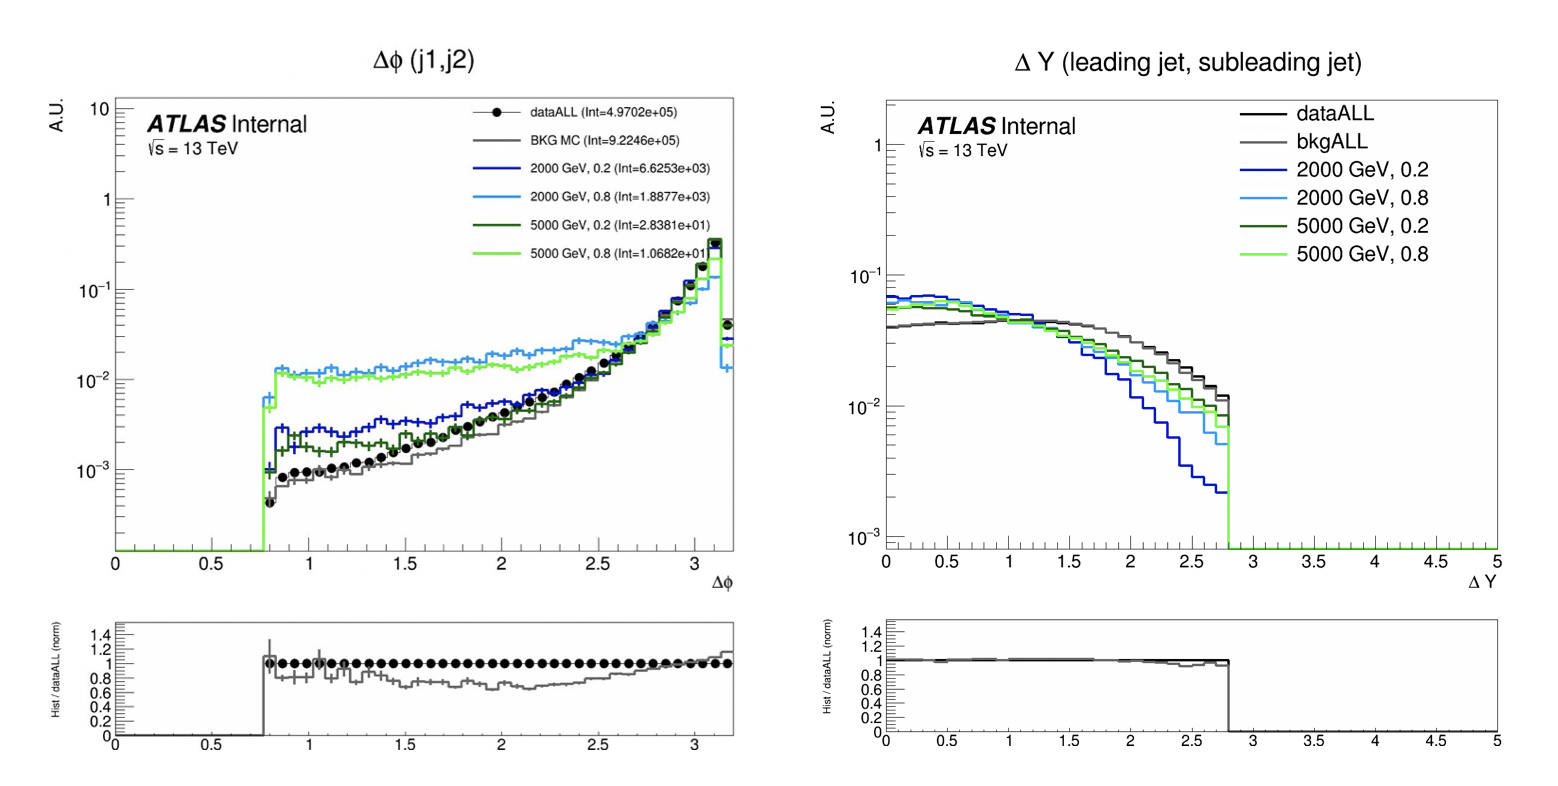
\includegraphics[width=0.95\textwidth]{figures/eventsel/preselection/presel3}
    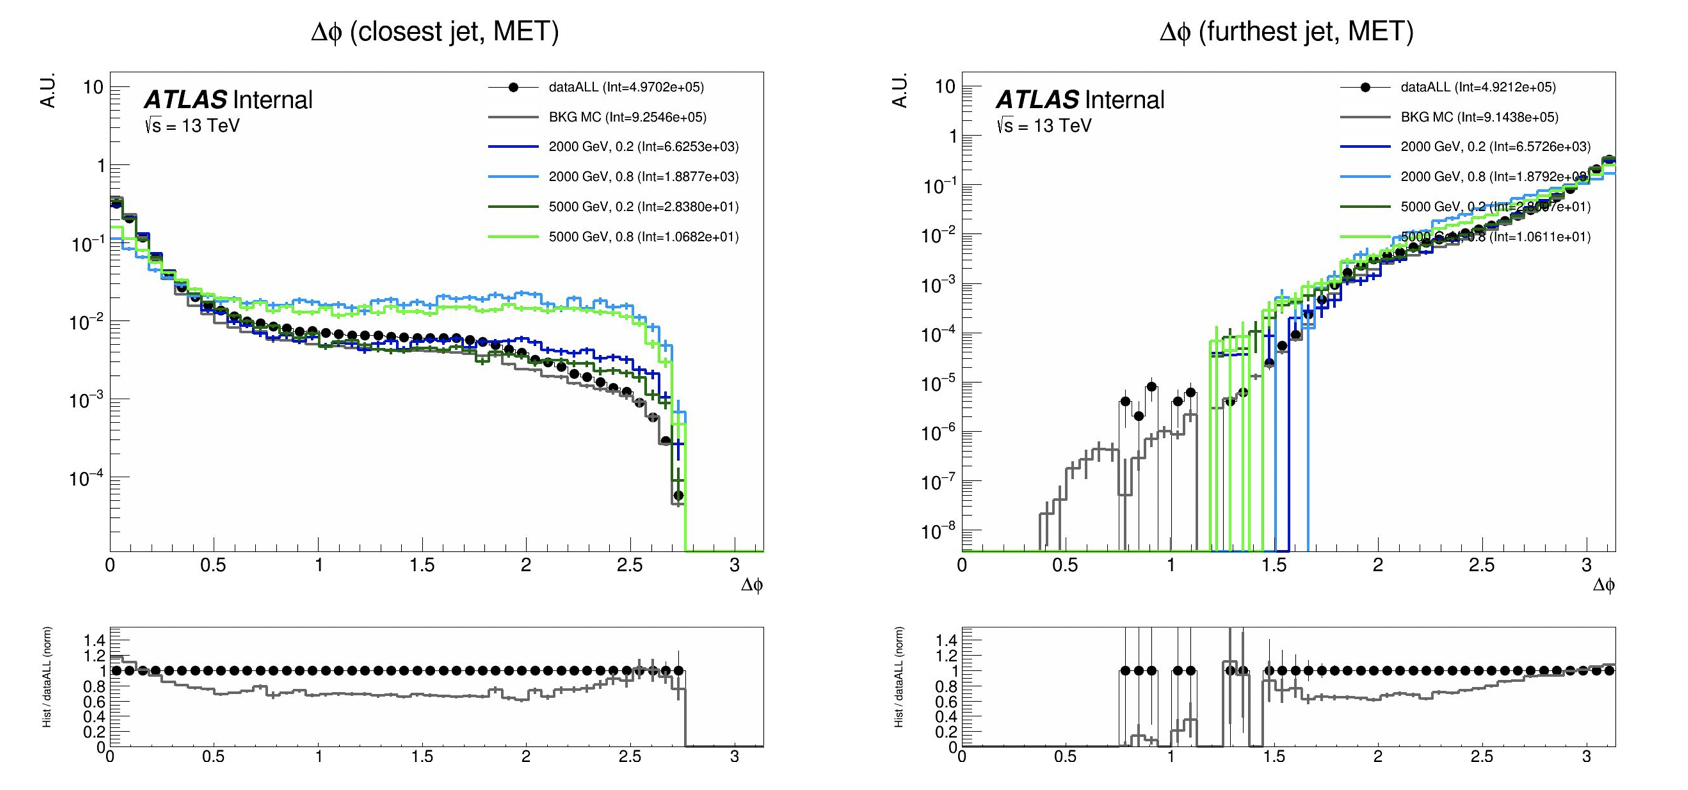
\includegraphics[width=0.95\textwidth]{figures/eventsel/preselection/presel4}
     \caption{Orientation analysis variables at preselection, for data (black), background MC (grey), and representative signal models (color). The signal models are identified in the legend as ``$m_{Z'}$, \rinv''. 
      \label{fig:presel_vars2}}
\end{figure}

The data and background MC are both illustrated in Figure~\ref{fig:presel_vars} and Figure~\ref{fig:presel_vars2}. The agreement between them is generally observed to be good, particularly in the key analysis variable \mt. The agreement is not required to be perfect as the background MC is not used for the background estimation. The primary motivation for studying the background MC is to uncover and remove issues unique to data such as the NCB, as described further in Appendix~\ref{app:ncb}.

 \clearpage
%\input{sections/object}


\section{SVJ Fit and Discovery Analysis Strategies}
\label{sec:strategies}
As was introduced in Chapter~\ref{ch:ml_tools} this analysis is interested in achieving dual goals: to make the best possible measurement of the SVJ signal model generated for this analysis, and to broadly search for any signals consistent with dark QCD behavior and inconsistent with a Standard-Model-only background hypothesis. To this end, two parallel analysis strategies are developed.\par

The SVJ Fit strategy uses the supervised PFN ML score in defining the signal region. Recall, the PFN is trained over simulated MC background and a combination of all MC SVJ signals. This gives this ML tool high sensitivity to the particular nuances of the SVJ shower predicted by the modeled theory. In addition to using the supervised ML tool, the SVJ Fit analysis strategy sets limits on the expected cross section of each signal point in the SVJ signal grid. To achieve this, the shape of the SVJ signals are considered in the final fit, as will be elaborated on Section~\ref{subsec:fit_exclusion}. The combination of the supervised PFN ML score and the signal-shape sensitive fitting strategy allows for the greatest possible sensitivity to the modeled signal process, thus allowing the analysis the best chance at discovery of this model, or enabling the analysis to set the best possible limits on the observed cross section.\par

In contrast, the Discovery analysis strategy attempts to design a more general search, which could be sensitive to SVJs, but also to other possible hidden valley dark QCD models, such as fully dark jets or emerging jets \cite{snowmass}. The Discovery analysis strategy uses the semi-supervised ANTELOPE ML score in defining the signal region. Recall, the ANTELOPE is trained over ATLAS data only, with no explicit knowledge of the SVJ signal behavior. The Discovery fit strategy is also signal model agnostic, by employing a bump hunt \cite{bumphunt} strategy, which searches a smoothly falling template for any bumps inconsistent with a background only hypothesis. Therefore any signal which could present a resonant signature in \mt~could show up as an excess in this strategy. \par

The details of both strategies will be explored in the follow sections which detail the design of the signal regions and fit strategies.
Figure~\ref{fig:fit_strategy} illustrates the difference in the fitting concept.
\begin{figure}[!htbp]
\centering
    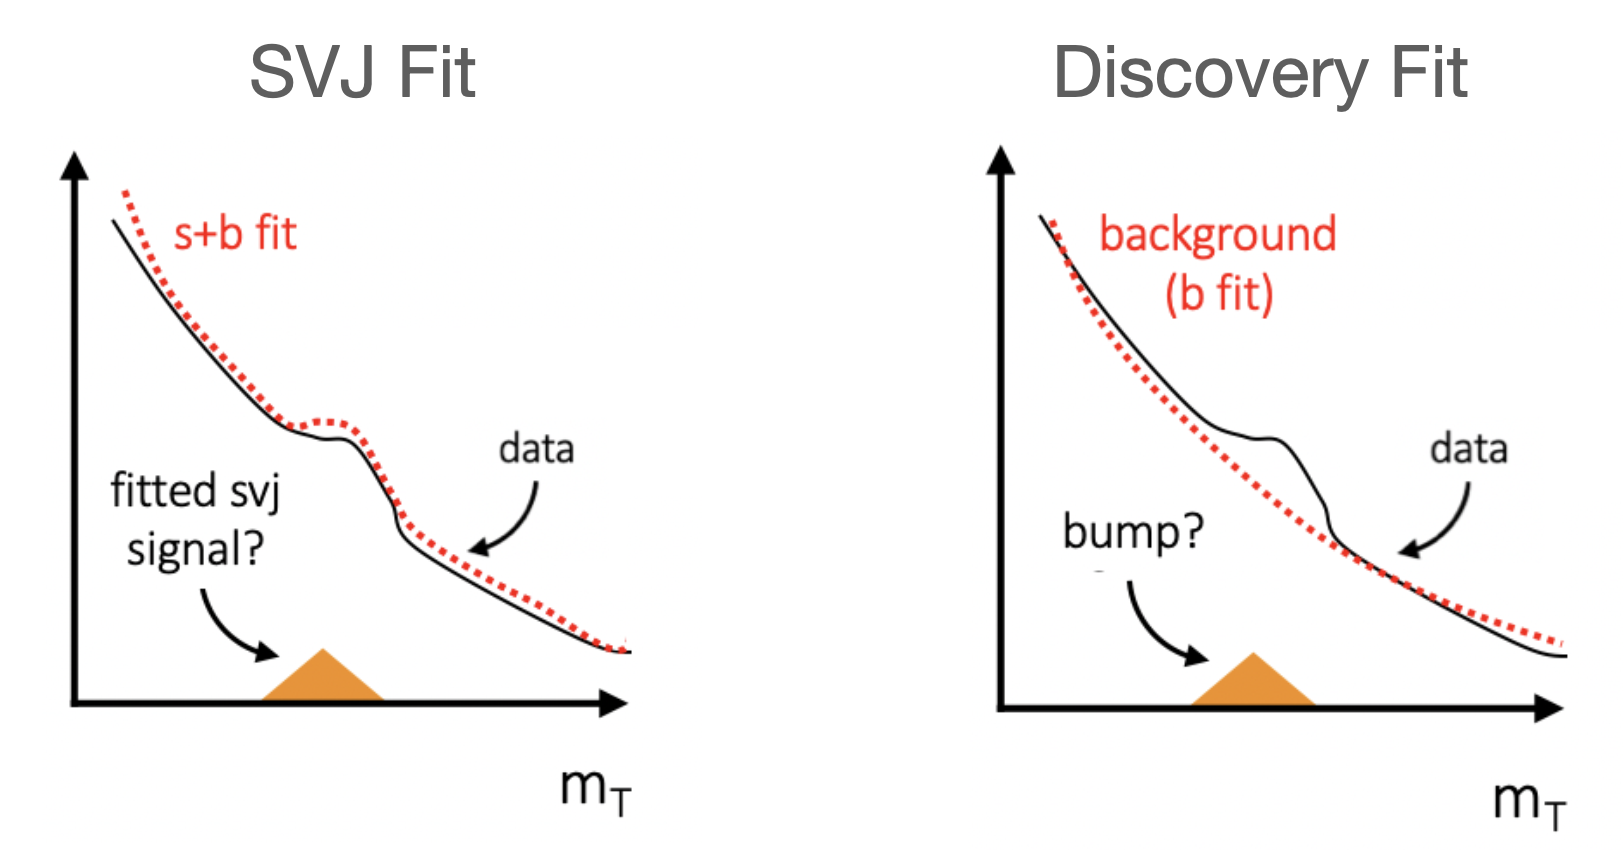
\includegraphics[width=0.5\textwidth]{figures/eventsel/fit_strategy}
    \caption{The two fitting strategies. The SVJ Fit (left) illustrates how SVJ signal shapes will be considered in the fit to search for SVJ specific signal shapes, where ``s+b fit'' indicates a fit that considers the shape of the signal. The Discovery Fit (right) illustrates how the data is compared to a background-only hypothesis to search for any kind of \mt~bump, where ``b fit'' indicates a background-only fit with no signal hypothesis.
    \label{fig:fit_strategy}}
\end{figure}

\section{Analysis Regions}
%------------------------------------------------- 
\subsection{Control and Validation Regions}
\label{subec:sel_crvr}

The final background estimation will come from a polynomial fit to the \mt~distribution in the signal region.
The control and validation regions are needed to develop and test this fit in data.
 
To define the CR selection, a variable is needed that isolates background from all signals across the (\rinv, $m_Z$) grid, which is challenging due to the varying nature of the signal models in quantities such as \met~and \pt~, as illustrated in Figure~\ref{fig:presel_vars}. 
The variable \textit{jet width} is chosen, which is the calorimeter measurement of the spread of the clusters which are used to define the jet ~\cite{jetwidth}.
The concept is illustrated in Figure~\ref{fig:jet2_calo}.
Jets with only one very energetic cluster have a small width, while jets with many lower energy clusters have a large width.
\begin{figure}[!htbp]
\centering
   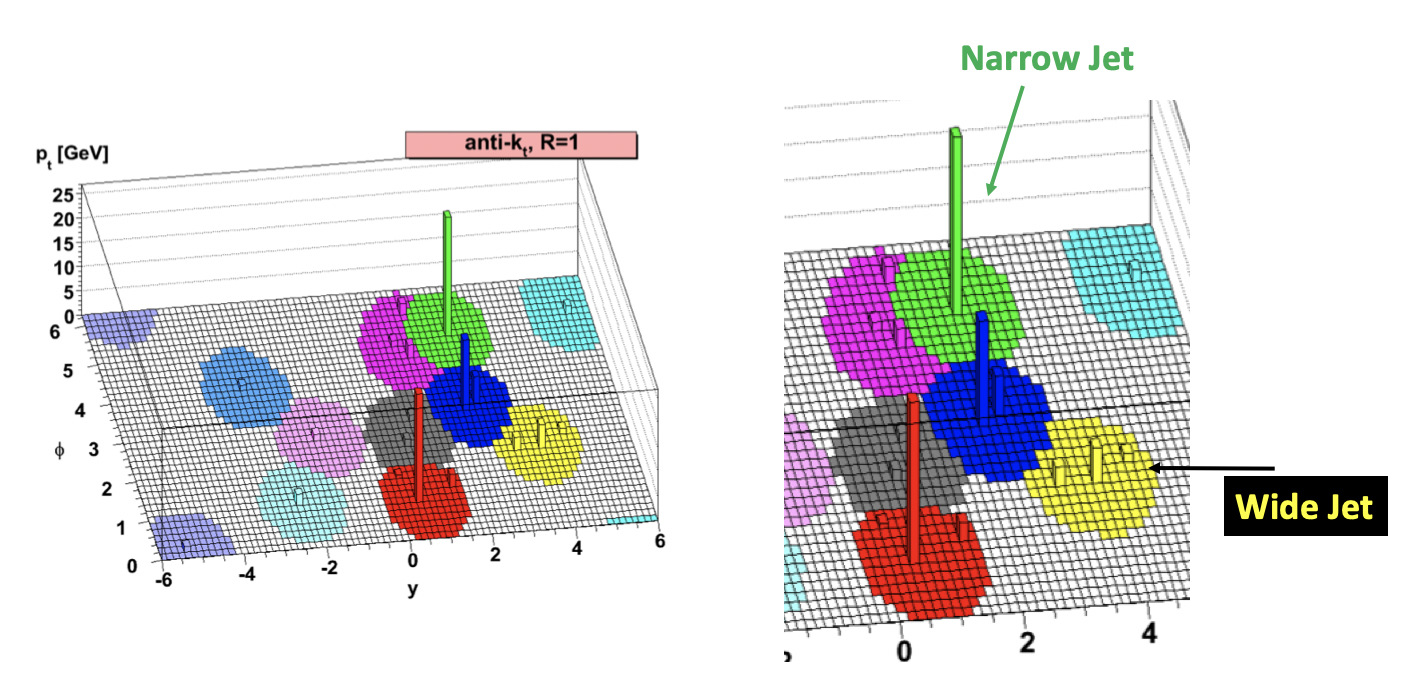
\includegraphics[width=0.95\textwidth]{figures/eventsel/jet2_calo}
    \caption{Recall the construction of anti-$k_t$ jets as described in Section~\ref{sec:jet_cluster} and illustrated in Figure~\ref{fig:jet_algorithms}. On the right, we zoom in on two jets, illustrating the narrow cluster pattern in the green jet, and the wide cluster pattern in the yellow jet.
    \label{fig:jet2_calo}}
\end{figure}

Figure~\ref{fig:jet2width} shows jet width specifically for the subleading jet, in data, background MC and signal at preselection.
The leading jet width, which was determined to be less useful for isolating signal from background is also shown.
The subleading jet is more likely to be aligned with \met, which is why the signal jet width is consistently wider in the subleading jet, but not the leading jet.  %, using v12 of the ntuples.
A selection of width$_{j2} <$ 0.05 is chosen for the CR, with the VR and SR therefore having a selection of width$_{j2}$ $\geq$ 0.05.
 
\begin{figure}[!htbp]
\centering
   %\includegraphics[width=0.4\textwidth]{figures/background/width$_{j2}$_datamc}
   \includegraphics[width=0.98\textwidth]{figures/background/jet2Width}
    \caption{Distributions of the subleading jet width width$_{j2}$ (left) and leading jet width width$_{j1}$ (right) in data, background MC and signals at preselection. All SVJ signals are seen to be wider than the background in width$_{j2}$. The same is not true for width$_{j1}$, where some signals are observed to closely match the background. 
    \label{fig:jet2width}}
\end{figure}

While the CR was used to develop the polynomial strategy, and is the primary region used in many of the fit studies, a validation region is used as an additional check of the estimation strategy in data.
The VR is defined using the region of events with low ML score by either the PFN or ANTELOPE networks.
Here the analysis strategy splits into the two parallel strategies presented in Section~\ref{sec:strategies}: the SVJ fit strategy and the Discovery strategy.
A selection of [PFN score $\leq$ 0.6 \& width$_{j2}$ $\geq$ 0.05] defines the SVJ Fit VR, while [ANTELOPE score $\leq$ 0.7 \& width$_{j2}$ $\geq$ 0.05] defines the discovery VR. 

There are therefore three variables that are crucial to the analysis strategy: width$_{j2}$, ML score, and \mt.
%Figure~\ref{fig:bkg_correlations} shows the correlations of all three variables to one another.
%Any outstanding correations are shown in Figure~\ref{fig:crvrsr_mt} to not sculpt the \mt~distribution and only affect its slope, making these variables trustworthy for extrapolation across background/signal regions and final fitting procedures.
%\begin{figure}[!htbp]
%\centering
 %  \includegraphics[width=0.95\textwidth]{figures/background/bkg_correlations}
 %  \includegraphics[width=0.95\textwidth]{figures/background/bkg_correlations_antelope}
 %   \caption{2D plots revealing correlations between width$_{j2}$ and \mt~(left), width$_{j2}$ and ML score (middle), and \mt~with ML score (right). For the top row, the ML score is the PFN score, and for the bottom three, the ML score is the ANTELOPE score. Minimal correlations are observed and are shown to not sculpt \mt, validating these variables for analysis region construction and statistical treatment.
%    \label{fig:bkg_correlations}}
%\end{figure}
We check the expected shape of \mt~across the CR, VR, and SR using background MC to ensure the shape is smoothly falling across all 3 regions.
Figure~\ref{fig:crvrsr_mt} shows the distribution of \mt~across the CR, VR, and SR, for both the PFN (supervised) and ANTELOPE (semi-supervised) strategies.
No significant bumps or sculpting are observed.
Some slope is observed in the ratio of the CR to the VR/SR shapes; however, the chosen background estimation strategy of polynomial fitting is expected to accommodate this slope.
Further, testing the ability of the background polynomial to fit shapes with a variety of slopes increases our confidence in the ability to background polynomial to fit the blinded SR \mt~distribution.%, which could be more problematic for a bump-hunt analysis.
\begin{figure}[!htbp]
\centering
   \includegraphics[width=0.98\textwidth]{figures/eventsel/mT_regions}
    \caption{\mt~in simulation across the CR, VR, and SR for both PFN (left) and ANTELOPE (right) selections. While there is variation in the slope of the distribution, no sculpting of bumps is observed.
    \label{fig:crvrsr_mt}}
\end{figure}

%------------------------------------------------- 
\subsection{Signal Region}
\label{subec:sel_sr}

A selection of PFN score $>$ 0.6 in the SVJ Fit region and ANTELOPE score $>$ 0.7 in the Discovery region is made to provide the primary signal-to-background enrichment, as motivated by Section~\ref{subsec:supervised}.
These values are determined to maximize $s/\sqrt{b}$ in each region.
The additional selection of {width$_{j2}$ $\geq$ 0.05} orthogonalizes the SR to the CR.
Note that the PFN and ANTELOPE regions are not orthogonal; this is because the two analysis flows serve different purposes, their statistical treatments are different, and they will not be combined. 

A summary of the SR, CR, and VR definitions can be seen in Figure~\ref{fig:crvrsr_2d}, along with the relative data statistics in each region.
\begin{figure}[!htbp]
\centering
    \includegraphics[width=0.98\textwidth]{figures/eventsel/crvrsr_2d}
    \caption{Distribution of data events amongst the CR, VR, and SR regions, along with the fractional population of each region. The SVJ Fit region is shown left with the PFN score on the x-axis, and Discovery region is shown right, with the ANTELOPE score on the x-axis.
    \label{fig:crvrsr_2d}}
\end{figure}

A diagram demonstrating the complete analysis flow can be seen in Figure~\ref{fig:analysisflow}.
\begin{figure}[!htbp]
\centering
    \includegraphics[width=1.1\textwidth]{figures/eventsel/analysisflow}
    \caption{Flow of analysis selections and fitting strategy. From preselection, events with Jet2Width < 0.05 are set aside for the CR. Events with Jet2Width $\geq$ 0.05 are split according the ML score. Events with low ML score create the VR, while events with high ML score create the SR. Events with high PFN score are fitted to determine if they are compatible with the SVJ signal shape. Events with high ANTELOPE score are fitted for a background estimation, and a search for any general data bump is performed.
    \label{fig:analysisflow}}
\end{figure}



\section{Background Estimation}
\label{sec:background}

%Backgrounds: The backgrounds should be evaluated and this should include CR/VR plots with the full data (full run-2 analyses) or at least a representative majority of the data (analyses during data-taking); 
%exceptionally a minor background could be still under finalization, but in this case a short timescale should be envisaged for its completion, or it should be a background that does not affect the accuracy of the result. ( a 10% background on a 10% accuracy measurement is not a minor background)

%This is done via a data template for the shape of \mt~taken from a CR that is orthogonal to the SR, but still close in SM process contribution and kinematic phase space. 
%A polynomial fit is then performed to describe the shape of \mt~in the SR.
%The polynomial is constructed using the CR data template, and validated to data in a VR that is similarly orthogonal to both the CR and SR.
The SM background in the SR is predominantly composed of QCD events, and due to the poor modeling of QCD at high energies by MC, it is estimated in a fully data-driven way. 
An empirical functional form is used for the background shape of \mt.
The ability of this function to model the background behavior is tested both the CR and the VR for each analysis strategy. The shape parameters are left free in all the fits.

The fits are performed for 1500 GeV $<$ \mt~ $<$ 6000 GeV.
The polynomial chosen is a standard 5-parameter function used in several similar dijet search analyses such as \cite{darkjets} \cite{smooth_bkg} \cite{cms_svj} and shown in Equation~\ref{eq:bkgpoly}:
\begin{equation}
f(x) = p_1(1-x)^{p_2}x^{p_3+p_4 lnx+p_5ln^2x}
\label{eq:bkgpoly}
\end{equation}
Here x = m$_{T}$/$\sqrt{s}$ (transverse mass scaled to the $pp$ collision center of mass energy), and $p_i$ are free parameters.
The fit function is required to be fully positive, and the \mt~distribution is fit to 90 even-width bins.
The resulting fit shape is used as the background estimation for both the SVJ Fit strategy and the Discovery strategy. 
Validation of the fit and its ability to both model the background and detect signal are shown in Section~\ref{sec:fit_strategy}.
Higher order polynomials were also considered, but an F-test was performed and the five parameter function was determined to be adequate and optimal for capturing the shape of the background.








\section{Fit Strategy and Validation}
\label{sec:fit_strategy}

The steps taken to validate the fitting approach for both the SVJ Fit strategy and the Discovery strategy will be outlined in the following sections. The signal region fits which compromise the final result will be presented in Chapter~\ref{ch:results},.

\subsection{SVJ Fit Strategy}
\label{subsec:fit_exclusion}

The ability of the five parameter fit function to capture the shape of the background is studied extensively, using data from the CR and VR. Signal injection tests are performed to determine the ability of the fit to recover and quantify any SVJ signal excess. Finally, estimates of the expected sensitivity are made. 
%Results: An overview of the final fit setup including the final discriminating variables(s), the (SR/CR) regions to be included in the fit and the floating normalization parameters. 
%Some rough first expected limits/discovery sensitivity plots are useful if you have them but not necessary. In this case the binning of the final variable(s) and the systematics smoothing/pruning should be indicated.


%------------------------------------------------- 
\subsubsection{Background Only Fits}
\label{subsec:fit_bkgonly}

Three validations are used for the background fit polynomial: MC across all analysis regions, data in the CR and VR, and pseudo-data in the CR and VR. 

Figure~\ref{fig:bkgfit_mc} shows the ability of this polynomial to fit the smoothly falling \mt~background in simulation across all 3 analysis regions (CR, VR, SR).
The \mt~spectrum is fit in 90 even bins.
These distributions are obtained by downsampling the MC statistics to match the relevant statistics of the data region, in accordance with the MC weights.
The high background-only $p$-value indicates a good fit.
\begin{figure}[!htbp]
\centering
   \includegraphics[width=0.95\textwidth]{figures/stats/bkgfit_mc}
    \caption{Background-only \mt~fits using representative MC in the CR (left), VR (middle), and SR (right).
    \label{fig:bkgfit_mc}}
\end{figure}

A slight sinusoidal pattern in the residuals may be observed. 
This arises due to the ``stitching" together of the \pt~slices for the QCD MC (as shown in Figure~\ref{fig:jzslices}), which is picked up by the fit.
For this reason, fitting to MC is only checked to verify that the differences in the slope of \mt~between the three regions (as shown in Figure~\ref{fig:crvrsr_mt}) do not pose a problem for the fitting strategy.

The nature of the functional fitting method allows it to easily adapt to changes in slope of a smoothly falling distribution.
Thus validation of the fit can be performed in data using the CR and the VR distributions to model the expected behavior in the SR. 
Figure~\ref{fig:bkgfit_data_fullstats} shows the a successful fit performed on the full statistics CR and VR regions.
\begin{figure}[!htbp]
\centering
   \includegraphics[width=0.82\textwidth]{figures/stats/bkgfit_data_fullstats}
    \caption{Background-only \mt~fits using data in the full statistics CR and VR regions.
    \label{fig:bkgfit_data_fullstats}}
\end{figure}

Figure~\ref{fig:postfit_param_pfn} shows the post-fit values of the fit parameters and their uncertainties for each fit. 
TODO: recalculate so it matches plot
\begin{figure}[!htbp]
\centering
   \includegraphics[width=0.65\textwidth]{figures/stats/postfit_param_pfn}
    \caption{Post-fit parameters for the PFN CR and VR.
    \label{fig:postfit_param_pfn}}
\end{figure}


Recall Figure~\ref{fig:crvrsr_2d}, which illustrates that the statistics of the CR and the VR are almost 3x the expected statistics of the SR.
The polynomial fitting strategy is sensitive to the statistics of the fitted template.
Its performance can very substantially depending on the statistical power of the fitted distribution.
To mitigate this, template \mt~histograms are obtained by randomly sampling the data in the CR/VR until a sample that is \textit{statistically identical} to the SR is obtained.
This process is referred to as \textit{downsampling}.
Examples of three downsampled histograms are provided for each region in Figure~\ref{fig:bkgfit_data}.
TODO: recalculate VR see if it's still bad
\begin{figure}[!htbp]
\centering
   %\includegraphics[width=0.32\textwidth]{figures/stats/dataDSfiveParFitChi2_CR0.png}
   %\includegraphics[width=0.32\textwidth]{figures/stats/dataDSfiveParFitChi2_CR1.png}
   %\includegraphics[width=0.32\textwidth]{figures/stats/dataDSfiveParFitChi2_CR2.png}
   %\includegraphics[width=0.32\textwidth]{figures/stats/dataDSfiveParFitChi2_VR0.png}
   %\includegraphics[width=0.32\textwidth]{figures/stats/dataDSfiveParFitChi2_VR1.png}
   %\includegraphics[width=0.32\textwidth]{figures/stats/dataDSfiveParFitChi2_VR2.png}
   \includegraphics[width=0.92\textwidth]{figures/stats/bkgfit_data_cr}
   \includegraphics[width=0.92\textwidth]{figures/stats/bkgfit_data_vr}
    \caption{Background-only \mt~fits using data in orthogonal but statistically identical samples to the SR, obtained by downsampling the CR/VR statistics, for the CR (top) and VR (bottom).
    \label{fig:bkgfit_data}}
\end{figure}

To further validate the fit stability of the fit against potential statistical fluctuations, \textit{pseudo-data} (also known as \textit{toy datasets}) are created from the CR data distribution. 
The pseudo-data is created following an \textit{Asimov} prescription \cite{asimov}, using a template to generate a set of toys representing different possible statistical fluctuations.
When studied as a group, the performance of the pseudo-data collection represents the range of possible behavior for an unknown distribution (the SR data in this case), given its statistical uncertainties.
The template used to generate the pseudo-data is a smoothed version of the CR. 
The smoothing applied follows the procedure for functional decomposition described in Ref.~\cite{edgar2018functional}.
Figure~\ref{fig:smoothing} shows the impact of smoothing on the source data distribution in the CR.
Toys are then generated from the smoothed distribution, by varying each bin within its statistical uncertainty according to a Poisson distribution. 
\begin{figure}[!htbp]
\centering
   \includegraphics[width=0.85\textwidth]{figures/stats/smoothing}
    \caption{\mt~distribution in the data CR, before (left) and after (right) smoothing.
    \label{fig:smoothing}}
\end{figure}

Figure~\ref{fig:asimov_hist} shows the resulting p-values after an ensemble of 100 Asimov pseudo-data are each individually fit. 
This test determines the likelihood of exceptionally good (high p-value) or poor (low p-value) fits due to randoms statistical fluctuations in the data. 
A flat distribution is observed, indicating good statistical behavior. 
\begin{figure}[!htbp]
\centering
   \includegraphics[width=0.45\textwidth]{figures/stats/asimov_cr_hist}
    \caption{$p$-value histograms from 100 fits to Asimov data in the CR. %, demonstrating a flat shape across p-value.
    \label{fig:asimov_hist}}
\end{figure}

%------------------------------------------------- 
\subsubsection{Signal + Background Fits}
\label{subsec:fit_splusb}

Figure~\ref{fig:splusb_sigInj} shows an example of an injected signal into the exclusion region \mt~spectrum, and the ability of the fit framework to accurately fit the number of signal events.
\begin{figure}[!htbp]
\centering
   \includegraphics[width=0.6\textwidth]{figures/stats/splusb_sigInj}
    \caption{Example S+B fits on a background \mt~spectrum with injected signal from the point (2500 GeV, \rinv=0.2).
    \label{fig:splusb_sigInj}}
\end{figure}

\paragraph{Signal Injection in Asimov Data}
To better understand the correlations of fit errors in the above single-template injection test and avoid drawing conclusions from a single scenario, signal injection tests using Asimov data will be performed before unblinding. 
50 Asimov trials are run for representative signal points across Z' mass and \rinv.

%Bias within the Asimov signal injection test could indicate a lack of sufficient normalization uncertainties on the signal model. 
%In the event of systematic mismeasurement in signal injection, the spurious signal uncertainty as derived from Loose-not-tight or additional uncertainties will be considered.

Figure~\ref{fig:siginj_asimov} provides the results of these tests. 
The uncertainty of the measurement varies according to mass point, due to the larger relative background for lower mass points. 
However, a strong linear relationship between amount of signal injected and amount of signal measured is observed for all signal points, which is the key feature.
\begin{figure}[!htbp]
\centering
   \includegraphics[width=0.45\textwidth]{figures/stats/siginj_asimov_02}
   \includegraphics[width=0.45\textwidth]{figures/stats/siginj_asimov_04}
   \includegraphics[width=0.45\textwidth]{figures/stats/siginj_asimov_06}
   \includegraphics[width=0.45\textwidth]{figures/stats/siginj_asimov_08}
   \caption{Measured signal at a variety of injected values (1x, 2x, and 5x$\sqrt{b}$), for all signal points in the grid, \rinv=0.2 (top left), 0.4 (top right), 0.6 (bottom left), and 0.8 (bottom right).
%he requirement relative to $\sigma_{\text{fit}}$ is met for every signal point and injected signal size, thus satisfying the OR criteria from Equation~\ref{eq:spursig}.
    \label{fig:siginj_asimov}}
\end{figure}

%------------------------------------------------- 
\subsubsection{Expected Sensitivity}
\label{subsec:fit_expsens}

Limits are obtained by determining the cross section of the signal that can be excluded to 95\% confidence. 
Figure~\ref{fig:limits_exp_1D} shows the expected limits obtained from S+B fits to statistically identical \mt~spectra from the CR region (which is closest in \mt~shape to the SR according to MC studies). 
%Figure~\ref{fig:limits_exp_1D_asimov} shows the expected limits obtained from an average of 50 Asimov toys thrown from the CR.
%The limits are very stable across individual data fits and Asimov, as well as across the CR and VR.
%The alignment of fluctuations between the single CR fit and Asimov toys indicates that the particular shape of data in the CR influences the shape of the limits.
%The limits shown come from an average of 10 Asimov pseudodata fits of the CR. Figure~\ref{fig:perc_success_limit} shows the percentage of Asimov limit tests that result in a successful fit. 

Considerable exclusion power is predicted for low \rinv~signal points, with the higher \rinv~points presenting more difficulty due to the very broad signal bump. 
A similar trend is observed in the CMS s-channel search~\cite{cms_schan}.

\begin{figure}[!htbp]
\centering
   \includegraphics[width=0.95\textwidth]{figures/stats/limits_exp_1D}
    \caption{95\% C.L. upper limits for signal models across Z' mass, for four different \rinv~fractions, from the CR region (without systematics).
    \label{fig:limits_exp_1D}}
\end{figure}
%\begin{figure}[!htbp]
%\centering
%   \includegraphics[width=0.9\textwidth]{figures/stats/limits_exp_1D_asimov_1}
%   \includegraphics[width=0.9\textwidth]{figures/stats/limits_exp_1D_asimov_2}
%    \caption{95\% C.L. upper limits for signal models across Z' mass, for four different \rinv~fractions, using an average of 50 Asimov pseudo-data tests from the CR (left) and VR (right) (without systematics).
%    \label{fig:limits_exp_1D_asimov}}
%\end{figure}

%\begin{figure}[!htbp]
%\centering
%   \includegraphics[width=0.6\textwidth]{figures/stats/perc_success_limit}
%    \caption{Percent of Asimov pseudodata S+B fits with successful fit and successful limit convergence.
%    \label{fig:perc_success_limit}}
%\end{figure}

A 2D limit presentation is also being considered, in the (\rinv, mass) plane.


\clearpage



%------------------------------------------------- 
\subsection{Discovery Strategy}
\label{subsec:fit_bh}

Model-independent fits for the discovery region are performed using \textsc{pyBumpHunter} \cite{bumphunt}.
The strategy consists of comparing the data in a given \mt~spectrum of interest to a background estimation derived by performing the polynomial fit and sampling from the post-fit function into a histogram.

The polynomial fit is done to an \mt~distribution with 180 bins (25 GeV wide), half the width of the fits in the SVJ Fit region (50 GeV wide). %90 bins, as with the PFN 
The narrower bins allow for rebinning based on the \textit{signal mass resolution} of the SVJ signals.
The binning strategy is outlined in Appendix~\ref{app:binning}.

Figure~\ref{fig:bkgfit_data_crvr_antelope} shows the fit and residuals with of the polynomial with the narrower binning in the CR and the Discovery VR data.
Figure~\ref{fig:postfit_param_antelope} shows the post-fit values of the fit parameters and their uncertainties for the CR and VR. 
These results indicate good ability of the 5-parameter polynomial to model the ANTELOPE selected data.

\begin{figure}[!htbp]
\centering
   \includegraphics[width=0.95\textwidth]{figures/stats/bkgfit_data_crvr_antelope}
    \caption{Post-fit function and residuals for the ANTELOPE CR and VR.
    \label{fig:bkgfit_data_crvr_antelope}}
\end{figure}

\begin{figure}[!htbp]
\centering
   \includegraphics[width=0.65\textwidth]{figures/stats/postfit_param_antelope}
    \caption{Post-fit parameters for the ANTELOPE CR and VR.
    \label{fig:postfit_param_antelope}}
\end{figure}

The studies shown in Section~\ref{subsec:fit_bkgonly} validate the robustness of the background polynomial fit. 
The narrower bins are the only difference for polynomial fitting between the SVJ Fit and Discovery Fit strategies, and they are not observed to reduce the quality or consistency of the fit. 

%----------------------------------------------------------------------------------------
\subsubsection{BumpHunter Fits}
\label{subsec:bhfits}

The signal mass resolution binning strategy described in Appendix~\ref{app:binning} creates a monotonically increasing set of bins. 
While the SVJ signals help inform the binning, the binning is still broadly applicable to a variety of potential signal models.
The mass resolution of any resonant signal generally widens as the mass of the mediator particle increases.
A similar strategy and binning was used in the generic heavy resonance search presented in Ref.~\cite{yxh}.
The resulting set of 15 bins to be used in the BumpHunter fits varies in width from 100 GeV at the \mt~core to 925 GV in the \mt~tail. 

Figure~\ref{fig:antelope_bh_crvr} shows the result of running BumpHunter over the rebinned CR and VR \mt~spectra.
The background estimation is given by polynomial fit function. 
The high p-values (>0.01) indicate good agreement with the background estimation.
\begin{figure}[!htbp]
\centering
   \includegraphics[width=0.95\textwidth]{figures/stats/antelope_bh_crvr}
    \caption{BumpHunter fits on the ANTELOPE \mt~spectra for both the CR (left) and VR (right). In a signal-depleted region, good agreement with the background estimation is observed.
    \label{fig:antelope_bh_crvr}}
\end{figure}

Figure~\ref{fig:bh_asimov_pvals} shows BumpHunter p-values over 100 Asimov trials, where each toy is scaled to the statistics of the SR.
The agreement is generally very good, as the p-values trend towards higher values.
No fits with a \textit{spurious signal} are found.
A spurious signal would be indicated by a fit with a p-value $<$ 0.01, indicting a bump of at least $2\sigma$ significance.
\begin{figure}[!htbp]
\centering
   \includegraphics[width=0.45\textwidth]{figures/stats/bh_asimov_pvals_cr}
   \includegraphics[width=0.45\textwidth]{figures/stats/bh_asimov_pvals_vr}
    \caption{BumpHunter p-values extracted for 100 Asimov toys for both the ANTELOPE CR (left) and VR (right).
    \label{fig:bh_asimov_pvals}}
\end{figure}

%----------------------------------------------------------------------------------------
\subsubsection{BumpHunter Signal Injection}
\label{subsec:bhsiginj}

To explore a model independent signal hypothesis, signal injection tests in the ANTELOPE region are done with generic Gaussian shapes.
Two Gaussian models are built with a mean ranging from 2000 GeV to 5000 GeV and a standard deviation equal to 10 or 20\% the mean value.
Figure~\ref{fig:gauss_inj} illustrates an injected Gaussian and its effect on the \mt~distribution.
The 20\% gaussian represents the widest possible signals we might be sensitive to with a BH strategy, while the 10\% injection represents a narrower signal peak. 

\begin{figure}[!htbp]
\centering
   \includegraphics[width=0.5\textwidth]{figures/stats/gauss_inj}
    \caption{Example injected gaussian signal.
    \label{fig:gauss_inj}}
\end{figure}

%The polynomial fit framework is run over background-only Asimov data to determine the injection level, as discussed in Section~\ref{subsec:fit_expsens}. 
%It should be noted that the $5\sigma$ injection level as determined by the polynomial fit is an underestimate, as the flexibility of the fit absorbs some of the signal.

An estimated $5\sigma$ of signal is injected for these tests.
The estimate is derived from the polynomial fitting framework, and is therefore an underestimate, as the flexibility of the polynomial fit absorbs some of the signal.
Therefore we do not expect to measure $5\sigma$ significance with the BH approach, but rather hope to see that some level of signal (at least $\geq2\sigma$ significance)  is observed by the BumpHunter framework. 

Results are obtained by averaging over 100 toys for each injection.
Figure~\ref{fig:siginj_bh} shows the resulting max local significance (in an \mt~bin) and the location of the determined bump, indicating a good response of the BumpHunter framework for detecting generic \mt~resonances at the right location.
Only the 5000 GeV 20\% width point is not properly identified by the framework. 
While some sensitivity is lost due to the flexible nature of the fitting framework, the ability to identify a bump with substantial local significance in the correct location is observed.
Figure~\ref{fig:bh_bump_example} shows an example of the identified bump.

\begin{figure}[!htbp]
\centering
   \includegraphics[width=0.65\textwidth]{figures/stats/siginj_bh_localsig.pdf}
   \includegraphics[width=0.65\textwidth]{figures/stats/siginj_bh_bumploc.pdf}
    \caption{Response of the BumpHunter framework to signal injection of $5\sigma$ significance to the model-dependent polynomial fit framework. The local significance (top) and bump location (bottom) are shown.
    \label{fig:siginj_bh}}
\end{figure}

\begin{figure}[!htbp]
\centering
   \includegraphics[width=0.5\textwidth]{figures/stats/bh_bump_example}
    \caption{Example BH response to gaussian signal injection at 4000 GeV with width of 10\%. 
    \label{fig:bh_bump_example}}
\end{figure}

%The BH significance can be slightly enhanced by repeating the polynomial fit after blinding the the most significant bump.
%This serves to ``flatten" the fit, allowing the bump to be more significant compared to the the background distribution. 
%This process is illustrated in Figure~\ref{fig:bh_masked}. 
%This strategy has the potential impact of enhancing non-signal deviations in the fit as well.
%Therefore, both BH results are considered together.

%\begin{figure}[!htbp]
%\centering
%   \includegraphics[width=0.95\textwidth]{figures/stats/bh_mask_before.pdf}
%   \includegraphics[width=0.95\textwidth]{figures/stats/bh_mask_after.pdf}
%    \caption{Improvement of the BH response after masking the region []redoing the polynomial background fit
%    \label{fig:siginj_bh}}
%\end{figure}



%%%%%%%%%%%%%%%%
% Chapter 9
%%%%%%%%%%%%%%%%
%\chapter{Results}
\label{ch:results}
The final results of this analysis are the polynomial fit to the \mt~distribution in the SVJ Fit SR, and the BumpHunter evaluation of the \mt~distribution in the Discovery SR. In the SVJ Fit region, systematic uncertainties are evaluated on the signal model, and \textit{limits}\footnote{A limit is an upper bound of the branching ratio of a signal process} on the observed $Z'$ production cross section are set. 

\section{SVJ Fit Result}
\label{sec:results_svj}
Figure~\ref{fig:unblinded_PFN_bonly} shows the unblinded \mt~spectrum in the SVJ Fit SR with a background-only fit. 
The fit is successful and has a p-value of 0.265, indicating the data is compatible with the background hypothesis. 
Table~\ref{tab:unblinded_params} gives the values and uncertainties for the five parameters of the polynomial fit function given in Equation~\ref{eq:bkgpoly}. 
\begin{figure}[!htbp]
\centering
   \includegraphics[width=0.5\textwidth]{figures/results/unblinded_PFN_bonly}
    \caption{\mt~in the unblinded SVJ Fit SR with a background-only fit (p-value = 0.265).
    \label{fig:unblinded_PFN_bonly}}
\end{figure}

\begin{table}[!htbp]
\centering
   \includegraphics[width=0.45\textwidth]{figures/results/postfit_param_pfnSR}
    \caption{Post-fit parameters for the PFN SR. $p1$ can also be considered $N_{bkg}$ or the normalization factor.
    \label{tab:unblinded_params}}
\end{table}

%Figure~\ref{fig:unblinded_limits_nosyst} shows the expected and observed limits in the unblinded SR, without signal systematics considered in the fit.
%As the data was found in the b-only fit to be compatible with background, good agreement of observed and expected limits is seen.
%\begin{figure}[!htbp]
%\centering
 %  \includegraphics[width=0.95\textwidth]{figures/results/unblinded_limits_nosyst}
 %   \caption{Expected and observed 95\% CL limits in the unblinded SR, as a function of Z' masses for \rinv=0.2 (top left), 0.4 (top right), 0.6 (bottom left), 0.8 (bottom right); no systematics.
%    \label{fig:unblinded_limits_nosyst}}
%\end{figure}

\subsection{Systematics}
\label{sec:syst}
As is typically done in dijet resonance searches using a polynomial fit \cite{dijet_uncert}, the systematic uncertainties in this analysis are applied only to the signal and not to the background.
This is because the background expectation is determined entirely from the data in the SR via the polynomial fit.
Therefore the only uncertainty on the background is the statistical uncertainty, which is reflected in the uncertainty associated to each of the five freely floating parameters determined in the fit.

A variety of systematics on the signal shape and yield are considered.
The most significant of these is the \textit{spurious signal} systematic, which quantifies the level of signal observed in the absence of signal injection.
Experimental uncertainties on the luminosity and jet reconstruction are studied.
Finally, uncertainties on the MC simulation of the SVJ theory model are also considered.

%------------------------------------------------------------
\subsubsection{Spurious Signal}

The spurious signal uncertainty is assessed following the prescription in Ref.~\cite{smooth_bkg}.
Asimov pseudo-datasets as described in Section~\ref{subsec:fit_bkgonly} are used to estimate the spurious signal.
The spurious signal uncertainty is included in the fit as a systematic uncertainty on the \textit{yield} of each signal point.

The spurious signal $\text{S}_{\text{spur}}$ is quantified for each signal as the mean number of signal events fitted across 100 signal-free pseudo-data experiments. 
To determine if the amount of spurious signal is tolerable, the threshold $\text{S}_{\text{spur}}$/$\sigma_{\text{fit}} < 0.5$ is used as recommended in Ref.~\cite{smooth_bkg}.
$\sigma_{\text{fit}}$ is the standard deviation on the number of fitted signal events for each signal point across the 100 pseudo-data experiments, and represents the statistical uncertainty on the number of fitted signal events.
The approximate total uncertainty on the fitted signal event yield is therefore $\sigma_\text{tot} \approx \sqrt{\sigma_\text{fit}^2 + \text{S}_\text{spur}^2}$ with the addition of the spurious signal systematic.
The requirement $\text{S}_{\text{spur}}$/$\sigma_{\text{fit}} < 0.5$ enforces that the increase in the total measurement uncertainty $\sigma_\text{tot}$ is tolerable at < 15\% ($\sqrt{1+0.5^2} \approx 1.12$ for $\text{S}_{\text{spur}} = 0.5\sigma_\text{fit}$).

%Figure~\ref{fig:spursig_nevents} shows the determined spurious signal as a function of Z' resonance mass, for both low and high \rinv~points.
Figure~\ref{fig:spursig} shows the $\text{S}_{\text{spur}}$/$\sigma_{\text{fit}}$ metric.
The requirement for $\text{S}_{\text{spur}}$/$\sigma_{\text{fit}}$ < 0.5 is easily satisfied across the signal grid.
\begin{figure}[!htbp]
\centering
   \includegraphics[width=0.6\textwidth]{figures/systs/spursig}
    \caption{Spurious signal metric as a function of resonance mass. The requirement $\text{S}_\text{spur}/\sigma_\text{fit} <0.5$ is satisfied for all signal points. 100 pseudo-data experiments are used for the measurement.
    \label{fig:spursig}}
\end{figure}

%As an additional verification of the size of the spurious signal, we perform the same check in the VR, as shown in Figure~\ref{fig:spursig_vs_mass_vr}.
%The size of the fitted spurious signal in the VR is consistent with that of the CR, indicating a good estimate of this uncertainty and extrapolation across regions.
%\begin{figure}[!htbp]
%\centering
%   \includegraphics[width=0.6\textwidth]{figures/systs/spursig_vs_mass_vr}
%    \caption{Fitted spurious signal in the VR, consistent with the CR and within the target size of $<$ 0.5 $\sigma$.
 %   \label{fig:spursig_vs_mass_vr}}
%\end{figure}

The average size of $\text{S}_{\text{spur}}$ is 209 events, and it ranges from 23 events for some \rinv~=0.2 signals to 470 events for some \rinv~=0.8 signals.
For most points the spurious signal uncertainty is about 50\% of the expected signal yield, though it ranges from 4.2\% for $m_{Z'}$ = 2000 to over 100\% for $m_{Z'}$ = 5000 GeV.
The experimental and theory uncertainties presented in the following sections are generally negligible in the fit due to the size of the spurious signal uncertainty.
They are included for completeness, and are significant for the $m_{Z'}$ = 2000 GeV, \rinv~= 0.2 and $m_{Z'}$ = 2500 GeV, \rinv~= 0.2 signal points, where the spurious signal uncertainty is < 5\%. 
%------------------------------------------------------------
\subsubsection{Experimental Uncertainties}
The main experimental uncertainties are on the recorded luminosity, \textit{jet energy scale}, and \textit{jet energy resolution}.
The jet energy scale (JES) corrects for the non-compensating calorimeter response and jet energy losses in passive detector material \cite{jes_jer}.
The jet energy resolution (JER) applies a correction based on the ratio between a jet's true energy and its reconstructed energy, as determined in simulation.
Systematics uncertainties on the JES and JER processes must be considered for any analysis using reconstructed jets.

A flat yield uncertainty of 0.83\% is applied for all signals, corresponding to the uncertainty reported on the luminosity measurement by the LUCID detector \cite{lucid_uncertainty}. 

The JES and JER uncertainties are evaluated on each signal point for their impact on both the yield and shape of the \mt~distribution.
Table~\ref{tab:exp_syst} summarizes the range impact on the yield for each uncertainty.
The impact of these uncertainties on the signal yield is generally very small in comparison to the spurious signal systematic.

\begin{table}
\centering
  \begin{tabular}{ |c|c| }
    \hline
    Uncertainty & Effect on Yield [\%] \\
    \hline
     Luminosity & 0.83 \\
     JES & 0.04 - 1.39 \\
     JER & 0.01 - 0.64 \\
    \hline
  \end{tabular}
  \caption{Summary of Experimental Uncertainties and their impact on the yield of MC signal events.}
  \label{tab:exp_syst}
\end{table}

The impact of the JES and JER uncertainties on the shape of the \mt~distribution is also considered.
An example individual JES variation is shown in Figure~\ref{fig:jes_uncert}, illustrating the minimal impact of this uncertainty on the shape of \mt.
The ``up'' and ``down'' variations refer to varying the nominal JES or JER setting by 1$\sigma$ up or down.
In principle these uncertainties can shift the mean of the \mt~distribution left or right, causing a substantial change in shape.
However, the impact of these uncertainties on the shape of \mt~in the SR is seen to be very small.
\begin{figure}[!htbp]
\centering
   \includegraphics[width=0.6\textwidth]{figures/results/jes}
    \caption{\mt~of the 3500 GeV $Z'$, \rinv~= 0.2 signal point, shown with an example JES uncertainty variation on the calorimeter noise. The nominal shape, 1$\sigma$ up, and 1$\sigma$ down variations are shown. The variation is seen to have minimal impact on the signal shape. Signal only (no background) is shown. 
    \label{fig:jes_uncert}}
\end{figure}

To make a conservative estimate of their impact on the shape, all shape uncertainty sources are summed in quadrature, bin-by-bin.
This results in a maximum 1$\sigma$ ``up'' variation and a maximum 1$\sigma$ ``down'' variation. 
The the impact of these maximal shape variations on the $Z'$ production cross section limit is evaluated, and uncertainty on this limit is propagated to the final limit bands. 
The impact is generally seen to be quite small, changing the limit variation by 0.61 fb at most. 
An example of the variations summed in quadrature is shown in Figure~\ref{fig:jetcp_sumq}. 
\begin{figure}[!htbp]
\centering
   \includegraphics[width=0.62\textwidth]{figures/results/jetcp_sumq}
    \caption{\mt~of the 3500 GeV $Z'$, \rinv~= 0.2 signal point, shown with the sum in quadrature of all JES and JER variations. The nominal shape before systematic variations, the maximal 1$\sigma$ ``up", and maximal 1$\sigma$ ``down" variations are shown. Even summed in quadrature, the effect of the JES and JER variations on the shape of the signal is seen to be small.
    \label{fig:jetcp_sumq}}
\end{figure}

%------------------------------------------------------------
\subsubsection{Theory Uncertainty}
Uncertainty on the parameters of the signal model are also considered. 
The primary theory uncertainty source is the tuning of the parton shower in \textsc{Pythia8} \cite{parton_shower}. 
Jet structure and extra jet production within the event depend on the modeling of initial state radiation (ISR), final state radiation (FSR) and behavior of multiple parton interactions (MPI) within an event.
A variety of MC generation tuning parameters govern the behavior of ISR, FSR and MPI in the signal generation.
Ref~\cite{pythia8_tunes} describes how these parameters are condensed into 10 variations which capture the maximal range of impact for these tuning parameters. 

The 10 variations (representing 5 up/down variation pairs) are evaluated for the SVJ signal shapes. 
Figure~\ref{fig:isrfsr} provides a look at the effect of these variations on the SVJ \mt~signal shape. 

\begin{figure}[!htbp]
\centering
   \includegraphics[width=0.9\textwidth]{figures/systs/isrfsr}
    \caption{Signal distribution of \mt, varying the ISR (Var1), FSR (Var2) and MPI (Var3a-c) configurations.
    \label{fig:isrfsr}}
\end{figure}

There is no substantial sculpting of the \mt~shape from any of the 10 systematic variations; thus the systematic is considered for its impact on the signal yield.
The variation in the signal yield is at most 1.2\%.
A conservative 2\% yield uncertainty is applied to account for the uncertainty on the theory model.
The spurious signal uncertainty is dominant for all but the lowest mass signal points.

%------------------------------------------------------------
\subsection{Interpretation}
Using a modified frequentist approach \cite{freq}, \textit{exclusion limits} at the 95\% confident level (CL) are derived.
The process was first described in Section~\ref{subsec:fit_expsens} and is reviewed here.
Exclusion limits refer to determining the maximum (or \textit{limiting}) signal cross section compatible with the observed data spectrum, such that any theory resulting in a signal cross section above the limit is excluded with 95\% confidence. 
The limit is determined from a maximum likelihood test statistic \cite{likelihood}, which determines the likelihood of observing the given data spectrum using the background hypothesis, signal hypothesis, and uncertainty parameters.
Compatibility of the signal model with the observed distribution is tested by generating pseudo-data based on the background estimation and including varying amounts of signal.
Through analysis of these pseudo-data experiments, the maximum number of signals events that is compatible with the observed data distribution can be determined.
The 95\% confidence level is enforced by dictating that the number of signal events must be compatible with the observed data within 2$\sigma$ of uncertainty.

The final limits on the $Z'$ cross section after the implementation of the systematic uncertainties are shown in Figure~\ref{fig:unblinded_limits_syst}. 
\begin{figure}[!htbp]
\centering
   \includegraphics[width=0.95\textwidth]{figures/results/final_limits}
    \caption{Expected and observed 95\% CL limits in the unblinded SR, as a function of $Z'$ mass for \rinv~= 0.2 (top left), 0.4 (top right), 0.6 (bottom left), 0.8 (bottom right).
    \label{fig:unblinded_limits_syst}}
\end{figure}
Exclusion of the theoretical model is observed for the 2000 GeV $Z'$ mass point for all \rinv~ values.
We are unable to exclude the highest mass points due to their low theoretical cross section, and relatively high spurious signal uncertainty.
The most mass points are excluded for \rinv~= 0.2, which excludes $Z'$ masses up to 3500 GeV.

\clearpage
%--------------------------------------------------------
\section{Discovery Result}
\label{sec:results_svj}
Figure~\ref{fig:unblinded_antelope_masked} shows the unblinded \mt~spectrum in the Discovery SR with a background-only fit, and the resulting BumpHunter test.
The polynomial fit is successful and has a background-only p-value of 0.74, indicating the data is compatible with the background hypothesis. 
The BumpHunter test gives a p-value of 0.8098, indicating no significant excess.
The maximum local significance is 0.877$\sigma$, located at 1700 GeV.

\begin{figure}[!htbp]
\centering
   \includegraphics[width=0.95\textwidth]{figures/results/unblinded_antelope_unmasked}
    \caption{\mt~in the unblinded ANTELOPE SR with a background-only fit (p-value = 0.74), left. BumpHunter test selecting the most significant data excess with a p-value of 0.8098, right.
    \label{fig:unblinded_antelope_masked}}
\end{figure}

Because there is no specific signal interpretation for the Discovery region and both the polynomial fit and BH analysis are entirely data driven, there are no systematics to consider in the interpretation of the BH result.
%To further characterize the ANTELOPE \mt~spectrum, the bin interval of most significant deviation as identified by the BumpHunter test is masked, and the fit is rerun.
%The resulting polynomial fit has an improved p-value of 0.86, as anticipated, indicating good fit response (Figure~\ref{fig:unblinded_antelope_masked}.
%\begin{figure}[!htbp]
%\centering
%   \includegraphics[width=0.5\textwidth]{figures/results/unblinded_antelope_masked}
%    \caption{\mt~in the unblinded and BH masked ANTELOPE SR with a new background-only fit (p-value = 0.86, indicating improved compatibility), left. BumpHunter test selecting the most significant data excess with a p-value of 0.8822 (eg. less significant than unmasked).
%    \label{fig:unblinded_antelope_unmasked}}
%\end{figure}



%%%%%%%%%%%%%%%%
% Conclusion
%%%%%%%%%%%%%%%%

\clearpage
\phantomsection
\addcontentsline{toc}{chapter}{Conclusion or Epilogue}

\begin{center}
\pagebreak
\vspace*{5\baselineskip}
\textbf{\large Conclusion or Epilogue}
\end{center}


\begin{flushleft}
\hspace{10mm}Use this page for your epilogue or conclusion if applicable; please use only one of the titles for this page. Otherwise, you may delete it.
Use this page for your epilogue or conclusion if applicable; please use only one of the titles for this page. Otherwise, you may delete it.
Use this page for your epilogue or conclusion if applicable; please use only one of the titles for this page. Otherwise, you may delete it.
Use this page for your epilogue or conclusion if applicable; please use only one of the titles for this page. Otherwise, you may delete it.
Use this page for your epilogue or conclusion if applicable; please use only one of the titles for this page. Otherwise, you may delete it.
Use this page for your epilogue or conclusion if applicable; please use only one of the titles for this page. Otherwise, you may delete it.
Use this page for your epilogue or conclusion if applicable; please use only one of the titles for this page. Otherwise, you may delete it.
Use this page for your epilogue or conclusion if applicable; please use only one of the titles for this page. Otherwise, you may delete it.
Use this page for your epilogue or conclusion if applicable; please use only one of the titles for this page. Otherwise, you may delete it.Use this page for your epilogue or conclusion if applicable; please use only one of the titles for this page. Otherwise, you may delete it.Use this page for your epilogue or conclusion if applicable; please use only one of the titles for this page. Otherwise, you may delete it.
Use this page for your epilogue or conclusion if applicable; please use only one of the titles for this page. Otherwise, you may delete it.Use this page for your epilogue or conclusion if applicable; please use only one of the titles for this page. Otherwise, you may delete it.
Use this page for your epilogue or conclusion if applicable; please use only one of the titles for this page. Otherwise, you may delete it.
Use this page for your epilogue or conclusion if applicable; please use only one of the titles for this page. Otherwise, you may delete it.
Use this page for your epilogue or conclusion if applicable; please use only one of the titles for this page. Otherwise, you may delete it.
Use this page for your epilogue or conclusion if applicable; please use only one of the titles for this page. Otherwise, you may delete it.
Use this page for your epilogue or conclusion if applicable; please use only one of the titles for this page. Otherwise, you may delete it.
Use this page for your epilogue or conclusion if applicable; please use only one of the titles for this page. Otherwise, you may delete it.
Use this page for your epilogue or conclusion if applicable; please use only one of the titles for this page. Otherwise, you may delete it.
Use this page for your epilogue or conclusion if applicable; please use only one of the titles for this page. Otherwise, you may delete it.
Use this page for your epilogue or conclusion if applicable; please use only one of the titles for this page. Otherwise, you may delete it.
Use this page for your epilogue or conclusion if applicable; please use only one of the titles for this page. Otherwise, you may delete it.Use this page for your epilogue or conclusion if applicable; please use only one of the titles for this page. Otherwise, you may delete it.Use this page for your epilogue or conclusion if applicable; please use only one of the titles for this page. Otherwise, you may delete it.
Use this page for your epilogue or conclusion if applicable; please use only one of the titles for this page. Otherwise, you may delete it.Use this page for your epilogue or conclusion if applicable; please use only one of the titles for this page. Otherwise, you may delete it.
Use this page for your epilogue or conclusion if applicable; please use only one of the titles for this page. Otherwise, you may delete it.
Use this page for your epilogue or conclusion if applicable; please use only one of the titles for this page. Otherwise, you may delete it.
Use this page for your epilogue or conclusion if applicable; please use only one of the titles for this page. Otherwise, you may delete it.
Use this page for your epilogue or conclusion if applicable; please use only one of the titles for this page. Otherwise, you may delete it.
Use this page for your epilogue or conclusion if applicable; please use only one of the titles for this page. Otherwise, you may delete it.
Use this page for your epilogue or conclusion if applicable; please use only one of the titles for this page. Otherwise, you may delete it.
Use this page for your epilogue or conclusion if applicable; please use only one of the titles for this page. Otherwise, you may delete it.
Use this page for your epilogue or conclusion if applicable; please use only one of the titles for this page. Otherwise, you may delete it.
Use this page for your epilogue or conclusion if applicable; please use only one of the titles for this page. Otherwise, you may delete it.
Use this page for your epilogue or conclusion if applicable; please use only one of the titles for this page. Otherwise, you may delete it.Use this page for your epilogue or conclusion if applicable; please use only one of the titles for this page. Otherwise, you may delete it.Use this page for your epilogue or conclusion if applicable; please use only one of the titles for this page. Otherwise, you may delete it.
Use this page for your epilogue or conclusion if applicable; please use only one of the titles for this page. Otherwise, you may delete it.Use this page for your epilogue or conclusion if applicable; please use only one of the titles for this page. Otherwise, you may delete it.
Use this page for your epilogue or conclusion if applicable; please use only one of the titles for this page. Otherwise, you may delete it.
Use this page for your epilogue or conclusion if applicable; please use only one of the titles for this page. Otherwise, you may delete it.
Use this page for your epilogue or conclusion if applicable; please use only one of the titles for this page. Otherwise, you may delete it.
Use this page for your epilogue or conclusion if applicable; please use only one of the titles for this page. Otherwise, you may delete it.
Use this page for your epilogue or conclusion if applicable; please use only one of the titles for this page. Otherwise, you may delete it.
Use this page for your epilogue or conclusion if applicable; please use only one of the titles for this page. Otherwise, you may delete it.
Use this page for your epilogue or conclusion if applicable; please use only one of the titles for this page. Otherwise, you may delete it.
Use this page for your epilogue or conclusion if applicable; please use only one of the titles for this page. Otherwise, you may delete it.
Use this page for your epilogue or conclusion if applicable; please use only one of the titles for this page. Otherwise, you may delete it.
Use this page for your epilogue or conclusion if applicable; please use only one of the titles for this page. Otherwise, you may delete it.Use this page for your epilogue or conclusion if applicable; please use only one of the titles for this page. Otherwise, you may delete it.Use this page for your epilogue or conclusion if applicable; please use only one of the titles for this page. Otherwise, you may delete it.
Use this page for your epilogue or conclusion if applicable; please use only one of the titles for this page. Otherwise, you may delete it.Use this page for your epilogue or conclusion if applicable; please use only one of the titles for this page. Otherwise, you may delete it.
Use this page for your epilogue or conclusion if applicable; please use only one of the titles for this page. Otherwise, you may delete it.
Use this page for your epilogue or conclusion if applicable; please use only one of the titles for this page. Otherwise, you may delete it.
Use this page for your epilogue or conclusion if applicable; please use only one of the titles for this page. Otherwise, you may delete it.
Use this page for your epilogue or conclusion if applicable; please use only one of the titles for this page. Otherwise, you may delete it.
Use this page for your epilogue or conclusion if applicable; please use only one of the titles for this page. Otherwise, you may delete it.
Use this page for your epilogue or conclusion if applicable; please use only one of the titles for this page. Otherwise, you may delete it.
Use this page for your epilogue or conclusion if applicable; please use only one of the titles for this page. Otherwise, you may delete it.
Use this page for your epilogue or conclusion if applicable; please use only one of the titles for this page. Otherwise, you may delete it.
Use this page for your epilogue or conclusion if applicable; please use only one of the titles for this page. Otherwise, you may delete it.
Use this page for your epilogue or conclusion if applicable; please use only one of the titles for this page. Otherwise, you may delete it.Use this page for your epilogue or conclusion if applicable; please use only one of the titles for this page. Otherwise, you may delete it.Use this page for your epilogue or conclusion if applicable; please use only one of the titles for this page. Otherwise, you may delete it.
Use this page for your epilogue or conclusion if applicable; please use only one of the titles for this page. Otherwise, you may delete it.Use this page for your epilogue or conclusion if applicable; please use only one of the titles for this page. Otherwise, you may delete it.
Use this page for your epilogue or conclusion if applicable; please use only one of the titles for this page. Otherwise, you may delete it.
\end{flushleft}


%\pagenumbering{gobble}  %remove page number on summary page





%%%%%%%%%%%%%%%%
% References
%%%%%%%%%%%%%%%%
\clearpage
\phantomsection 
\titleformat{\chapter}[display]
{\normalfont\bfseries\filcenter}{}{0pt}{\large\bfseries\filcenter{#1}}  % Reset title format for Reference section. (It is different from Chapter titles)
\titlespacing*{\chapter}
  {0pt}{0pt}{30pt}

\begin{singlespace}  % use single-line spacing for multi-line text within a single reference
	\setlength\bibitemsep{\baselineskip}  %manually set separataion betwen items in bibliography to double space
	\addcontentsline{toc}{chapter}{References}  %add References section to Table of Contents
	\printbibliography[title={References}]
\end{singlespace}



%%%%%%%%%%%%%%%%
% Appendices
%%%%%%%%%%%%%%%%

%Readjust Title format for Appendicies
\titleformat{\chapter}[display]
{\normalfont\bfseries\filcenter}{}{0pt}{\large\chaptertitlename\ \large\thechapter : \large\bfseries\filcenter{#1}}  
\titlespacing*{\chapter}
  {0pt}{0pt}{30pt}	%controls vertical margins on title
  
% Adjust section title formatting
\titleformat{\section}{\normalfont\bfseries}{\thesection}{1em}{#1}

% Adjust subsection title formatting
\titleformat{\subsection}{\normalfont}{\thesubsection}{0em}{\hspace{1em}#1}

\begin{appendices}

%Some Table of Contents entry formatting
\addtocontents{toc}{\protect\renewcommand{\protect\cftchappresnum}{\appendixname\space}}
\addtocontents{toc}{\protect\renewcommand{\protect\cftchapnumwidth}{6em}}

%Begin individual appendices, separated as chapters

\chapter{ Experimental Equipment}
Lorem ipsum dolor sit amet, consectetur adipiscing elit, sed do eiusmod tempor incididunt ut labore et dolore magna aliqua. Ut enim ad minim veniam, quis nostrud exercitation ullamco laboris nisi ut aliquip ex ea commodo consequat. Duis aute irure dolor in reprehenderit in voluptate velit esse cillum dolore eu fugiat nulla pariatur. Excepteur sint occaecat cupidatat non proident, sunt in culpa qui officia deserunt mollit anim id est laborum.

\chapter{Data Processing}
Lorem ipsum dolor sit amet, consectetur adipiscing elit, sed do eiusmod tempor incididunt ut labore et dolore magna aliqua. Ut enim ad minim veniam, quis nostrud exercitation ullamco laboris nisi ut aliquip ex ea commodo consequat. Duis aute irure dolor in reprehenderit in voluptate velit esse cillum dolore eu fugiat nulla pariatur. Excepteur sint occaecat cupidatat non proident, sunt in culpa qui officia deserunt mollit anim id est laborum.

\end{appendices}

\end{document} 
